\documentclass[a4paper,12pt]{article}
\usepackage{graphicx}
\usepackage{amsmath, amssymb}
\usepackage{siunitx}
\usepackage{float}
\usepackage{caption}
\usepackage{subfigure}
\usepackage{array}

\title{\textbf{Experiment-06-Bandpass Filter using Sallen-Key Second-Order Filters}}
\author{EE24BTECH11048-NITHIN.K\\ EE24BTECH11021-ESHAN RAY}
\date{\today}

\begin{document}

\maketitle

\section{Objective}
\begin{enumerate}
    \item To design and implement a bandpass filter using separate Sallen-Key Low Pass Filter (LPF) and High Pass Filter (HPF).
    \item To analyze and compare the frequency response of LPF, HPF, and the final bandpass filter.
    \item To plot the magnitude response (gain vs. frequency) of all three filters.
\end{enumerate}

\section{Theory}
A bandpass filter (BPF) allows frequencies within a specified range while attenuating those outside it. It is constructed using:
\begin{itemize}
    \item A High Pass Filter (HPF) to remove low-frequency components.
    \item A Low Pass Filter (LPF) to remove high-frequency components.
    \item The combined response results in a bandpass characteristic.
\end{itemize}

Sallen-Key Second-Order Filters use operational amplifiers to provide different responses such as Butterworth, Bessel, or Chebyshev depending on component selection. The transfer function is:
\begin{equation}
    H(s) = \frac{A}{s^2 + \frac{\omega_c}{Q}s + \omega_c^2}
\end{equation}
where:
\begin{itemize}
    \item $\omega_c$ is the cutoff frequency.
    \item $Q$ is the quality factor.
\end{itemize}

\section{Circuit Design}
\subsection{High Pass Filter (HPF) Design}
A high pass filter allows signals with frequencies higher than a certain cutoff frequency to pass while attenuating lower frequencies. The cutoff frequency $f_{c1}$ is given by:
\begin{equation}
    f_{c1} = \frac{1}{2\pi \sqrt{R_1 R_2 C_1 C_2}}
\end{equation}
This filter is used to eliminate unwanted low-frequency noise, such as DC offsets, and isolate higher-frequency components.\\
\textbf{The values of Resistors are:} 14.8kohm, 14.8kohm \\
\textbf{The values of Capacitors are:} 1nF, 1.2nF \\
\begin{figure}[H]
    \centering
    \subfigure[]{
        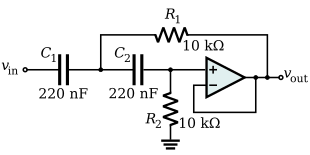
\includegraphics[width=0.45\textwidth]{figs/highpass.png}
    }
    \hfill
    \subfigure[]{
        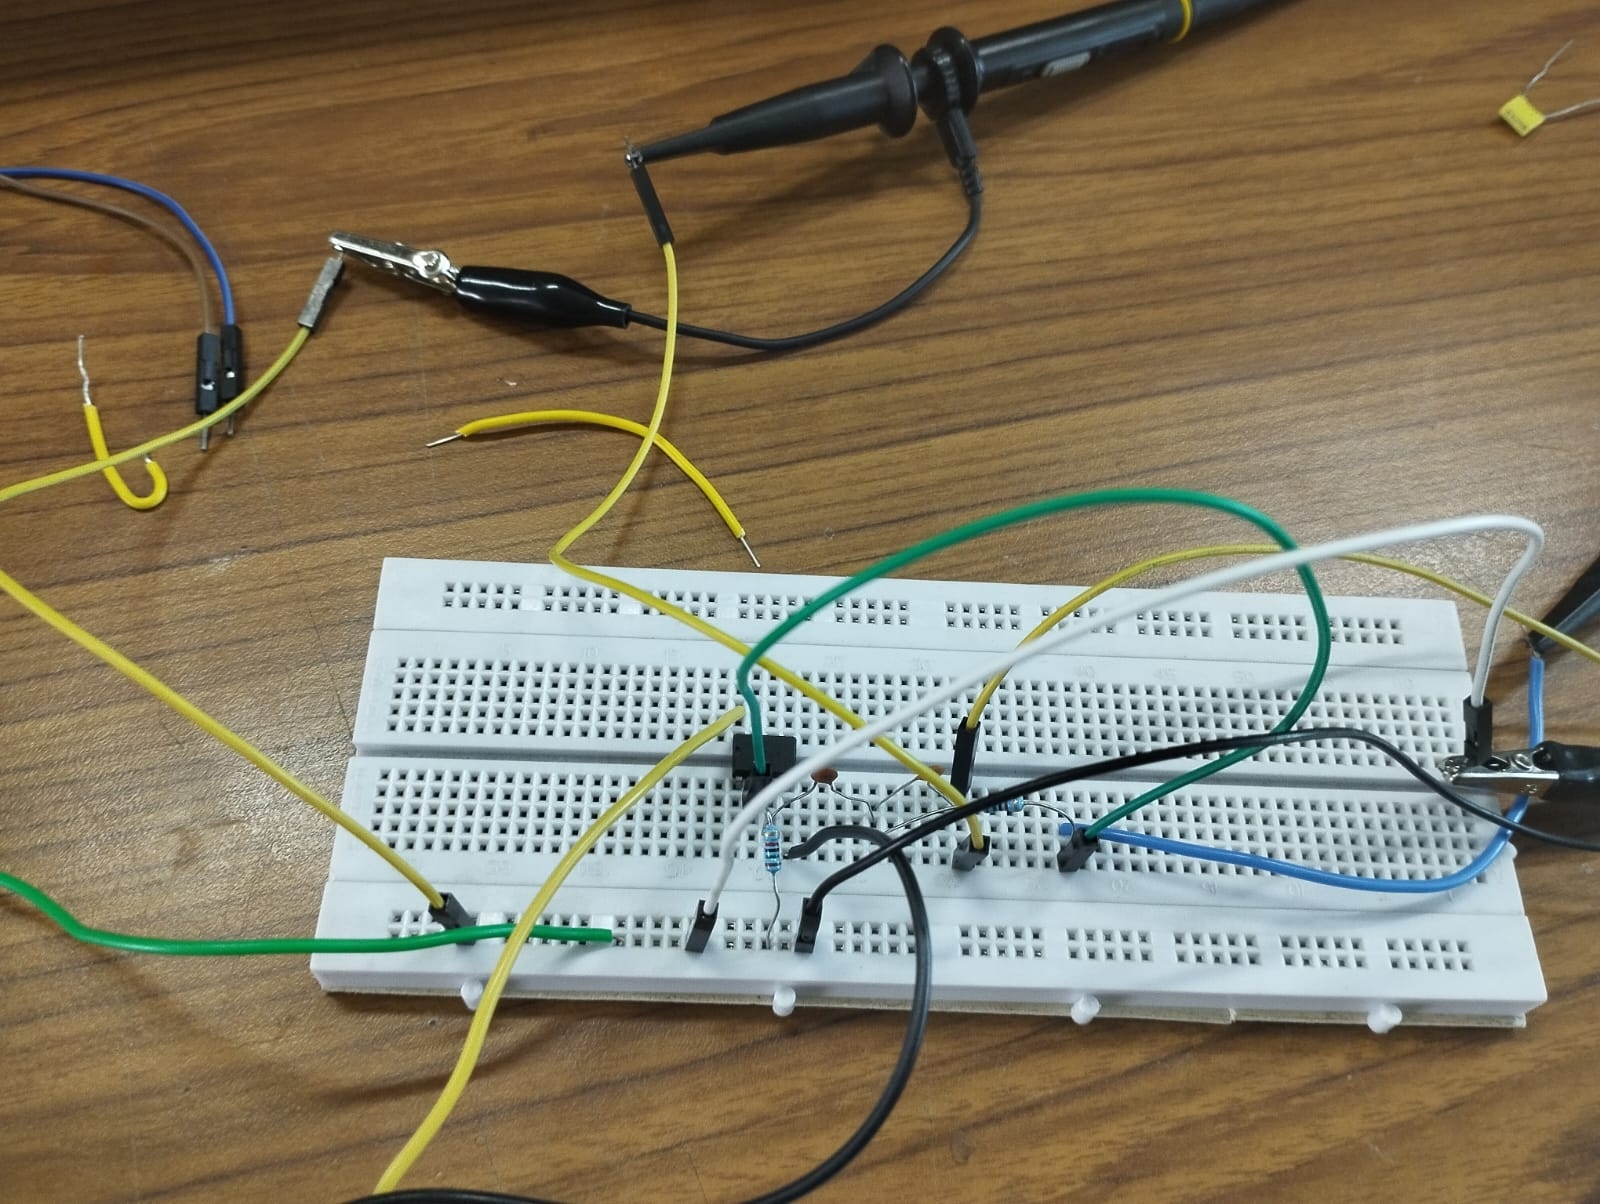
\includegraphics[width=0.45\textwidth]{figs/hpf_circuit.jpeg}
    }
\end{figure}
\begin{table}[H]
    \centering
    \renewcommand{\arraystretch}{1.3} % Adjust row height
    \begin{tabular}{|c|c|c|}
        \hline
        \textbf{S. No.} & \textbf{Input Frequency (Hz)} &\textbf{Output Voltage (V)} \\
        \hline
        1 & 100 & 0.54  \\
        2 & 500 & 0.56  \\
        3 & 1000 & 0.56  \\
        4 & 5000 & 0.56  \\
        5 & 10000 & 0.66  \\
        6 & 25000 & 0.8  \\
        7 & 50000 & 0.96  \\
        8 & 100000 & 0.96  \\
        \hline
    \end{tabular}
    \caption{Observation Table for Frequency Response for HPF}
    \label{tab:observation}
\end{table}

\begin{figure}[H]
    \centering
    \subfigure[]{
        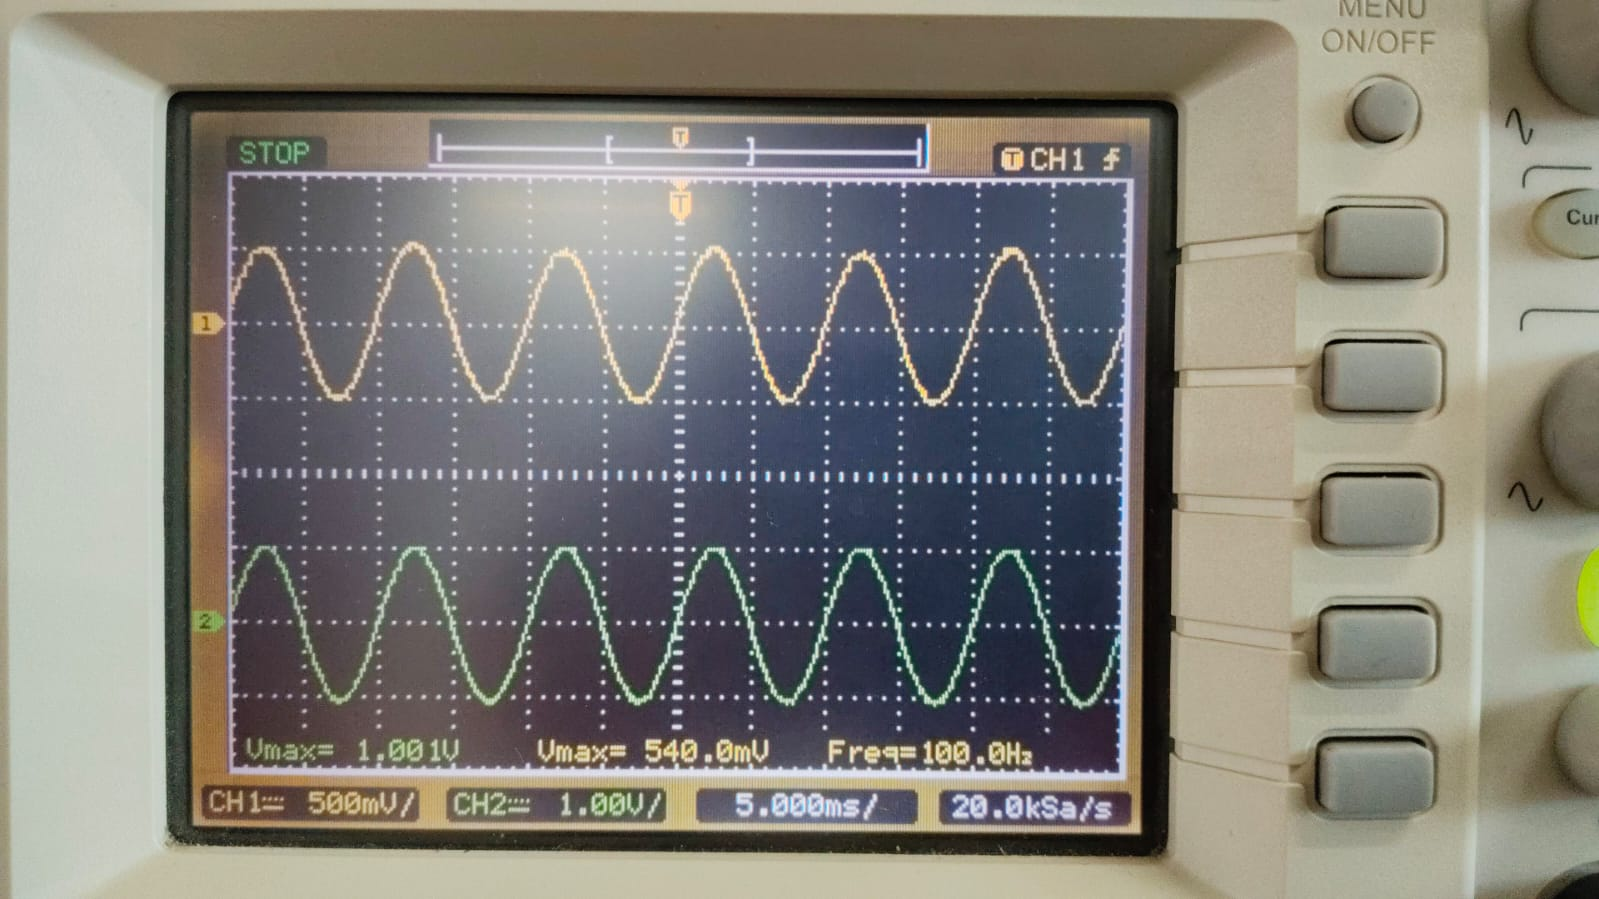
\includegraphics[width=0.45\textwidth]{figs/hpf_less_cutoff_4.jpeg}
    }
    \hfill
    \subfigure[]{
        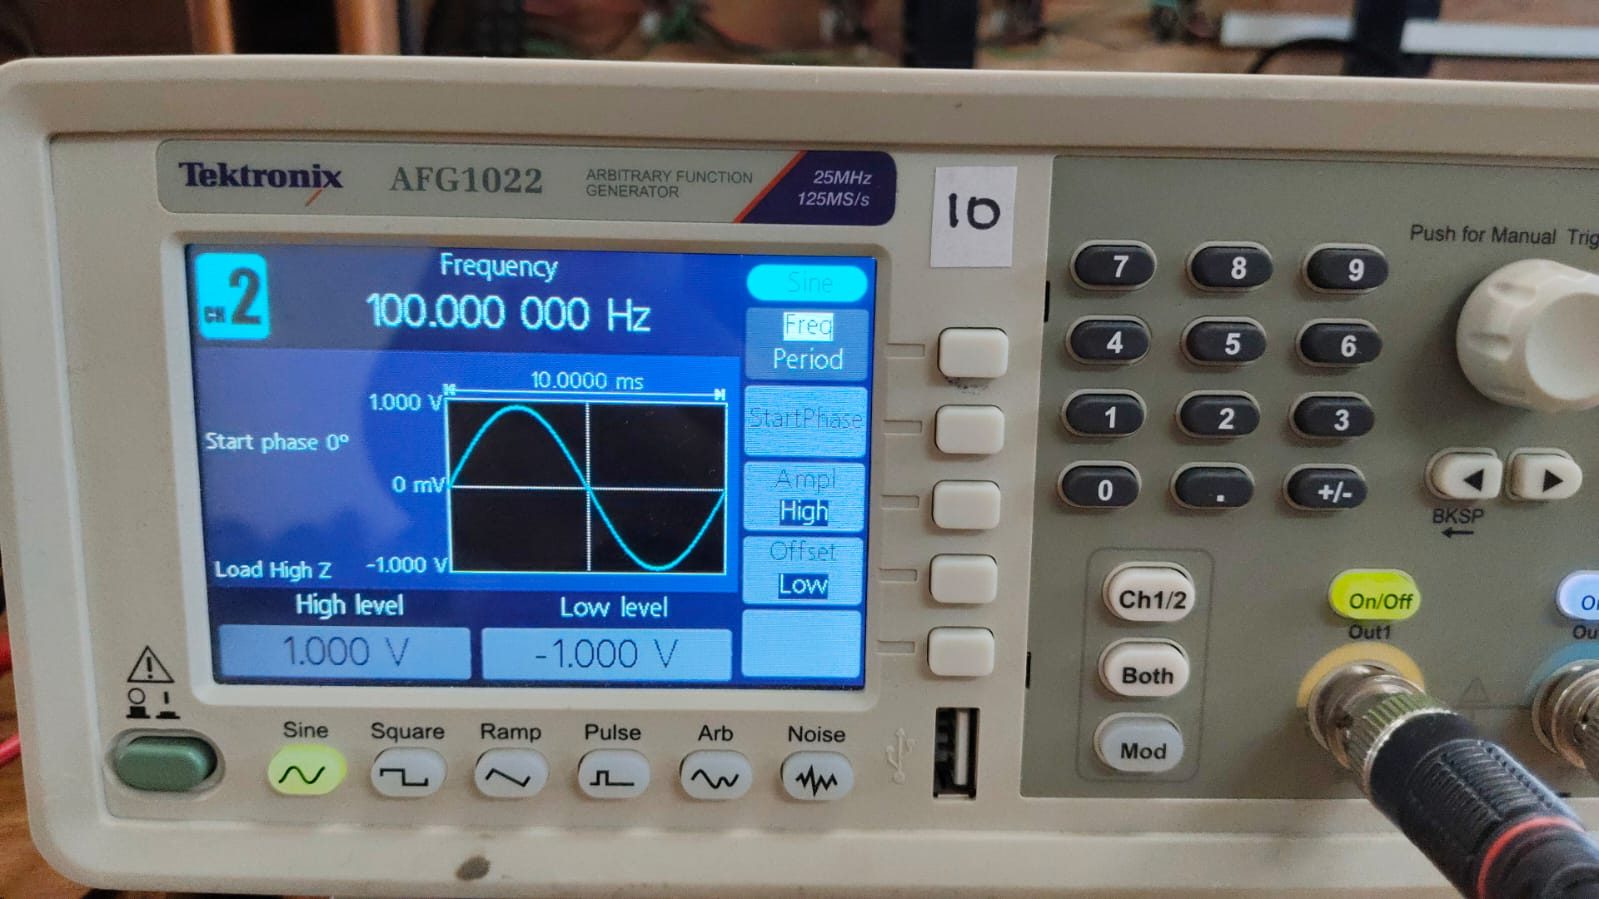
\includegraphics[width=0.45\textwidth]{figs/hpf_input_less_cutoff_4.jpeg}
    }
\end{figure}
\begin{figure}[H]
    \centering
    \subfigure[]{
        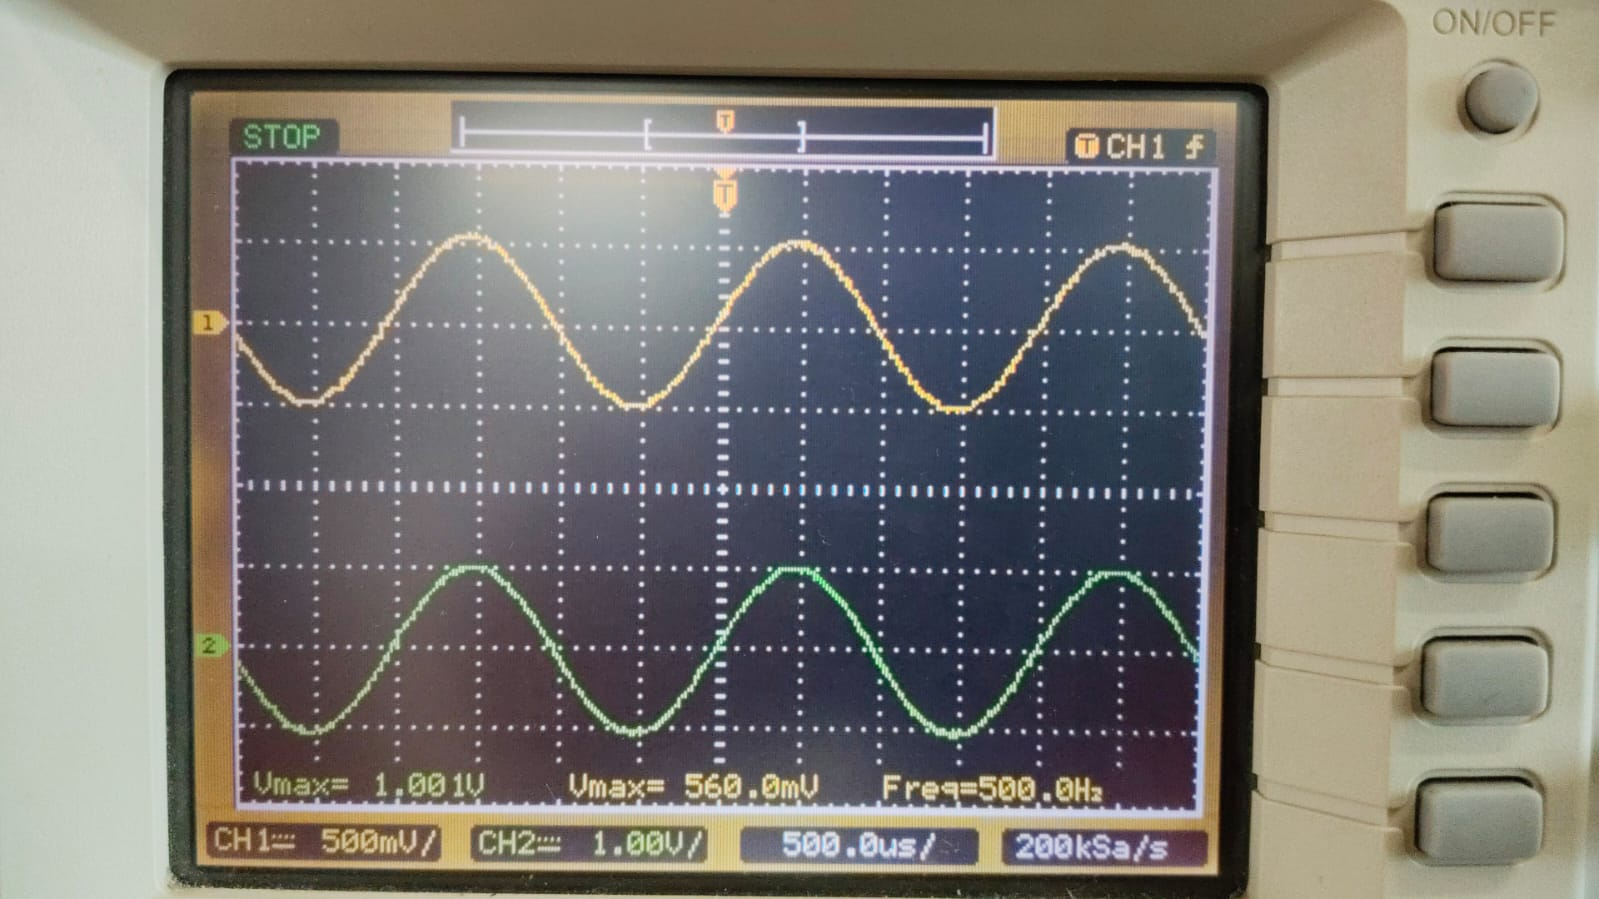
\includegraphics[width=0.45\textwidth]{figs/hpf_less_cutoff_3.jpeg}
    }
    \hfill
    \subfigure[]{
        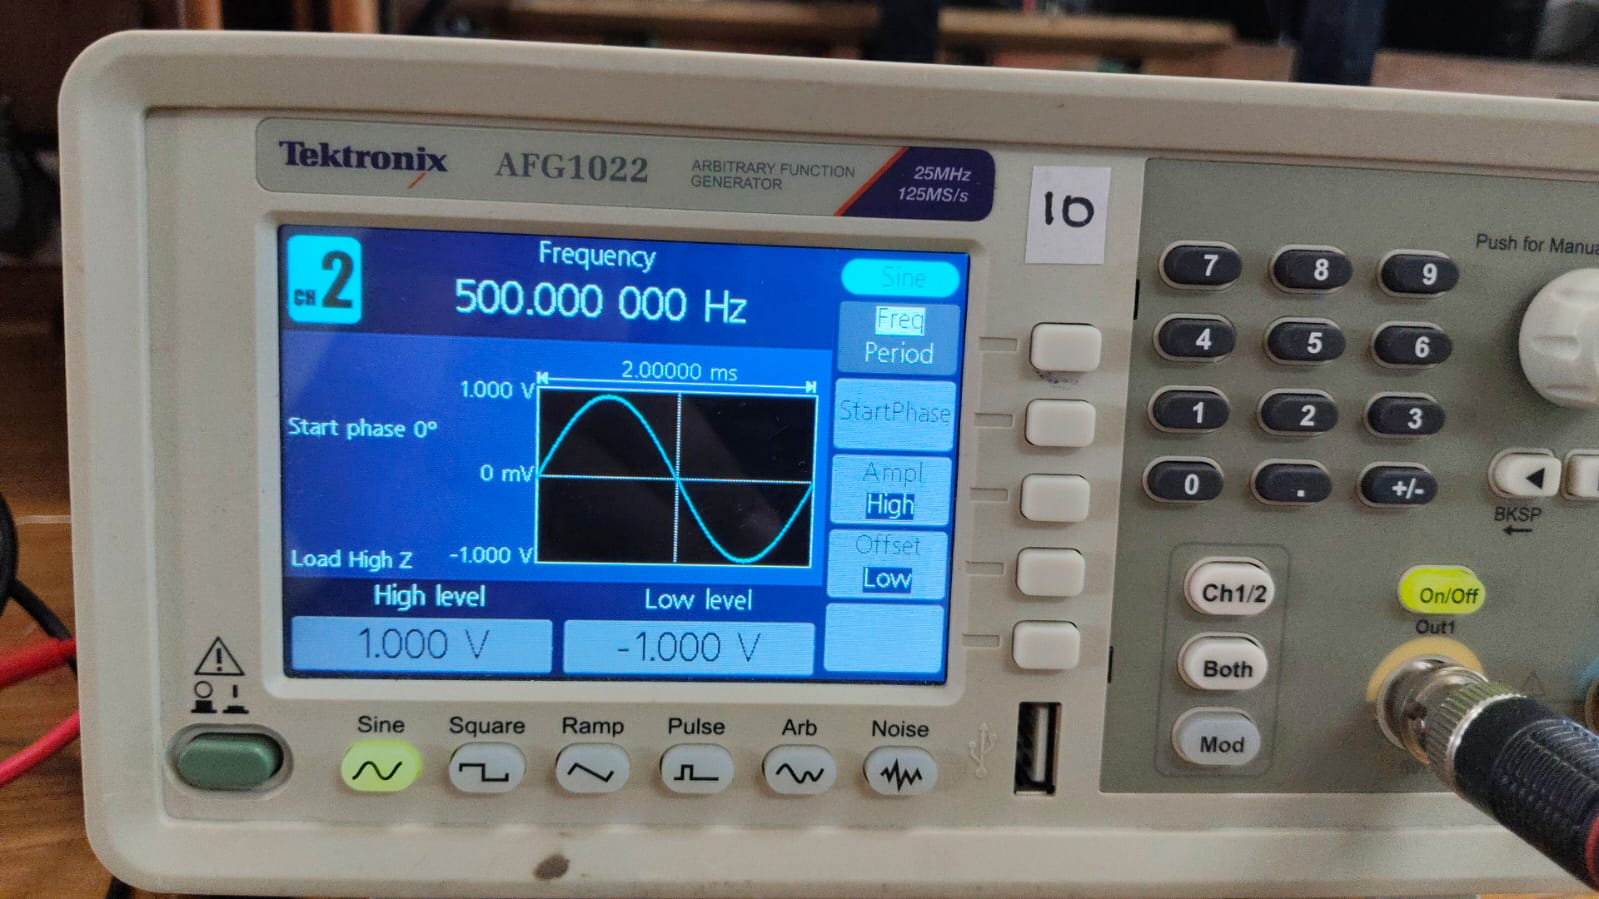
\includegraphics[width=0.45\textwidth]{figs/hpf_input_less_cutoff_3.jpeg}
    }
\end{figure}
\begin{figure}[H]
    \centering
    \subfigure[]{
        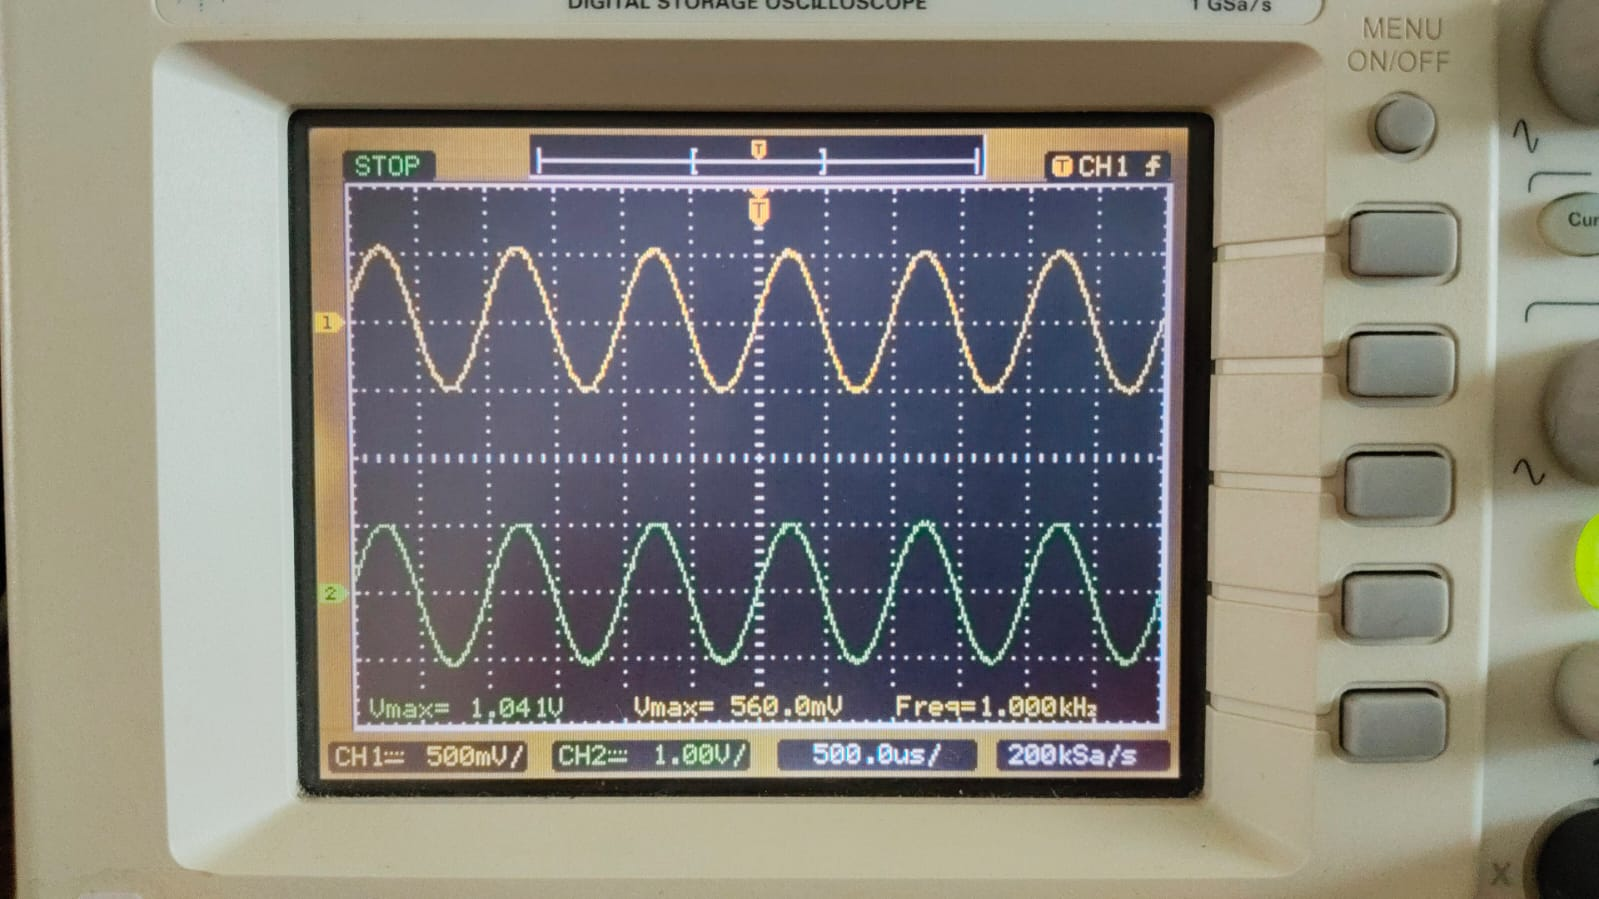
\includegraphics[width=0.45\textwidth]{figs/hpf_less_cutoff_1.jpeg}
    }
    \hfill
    \subfigure[]{
        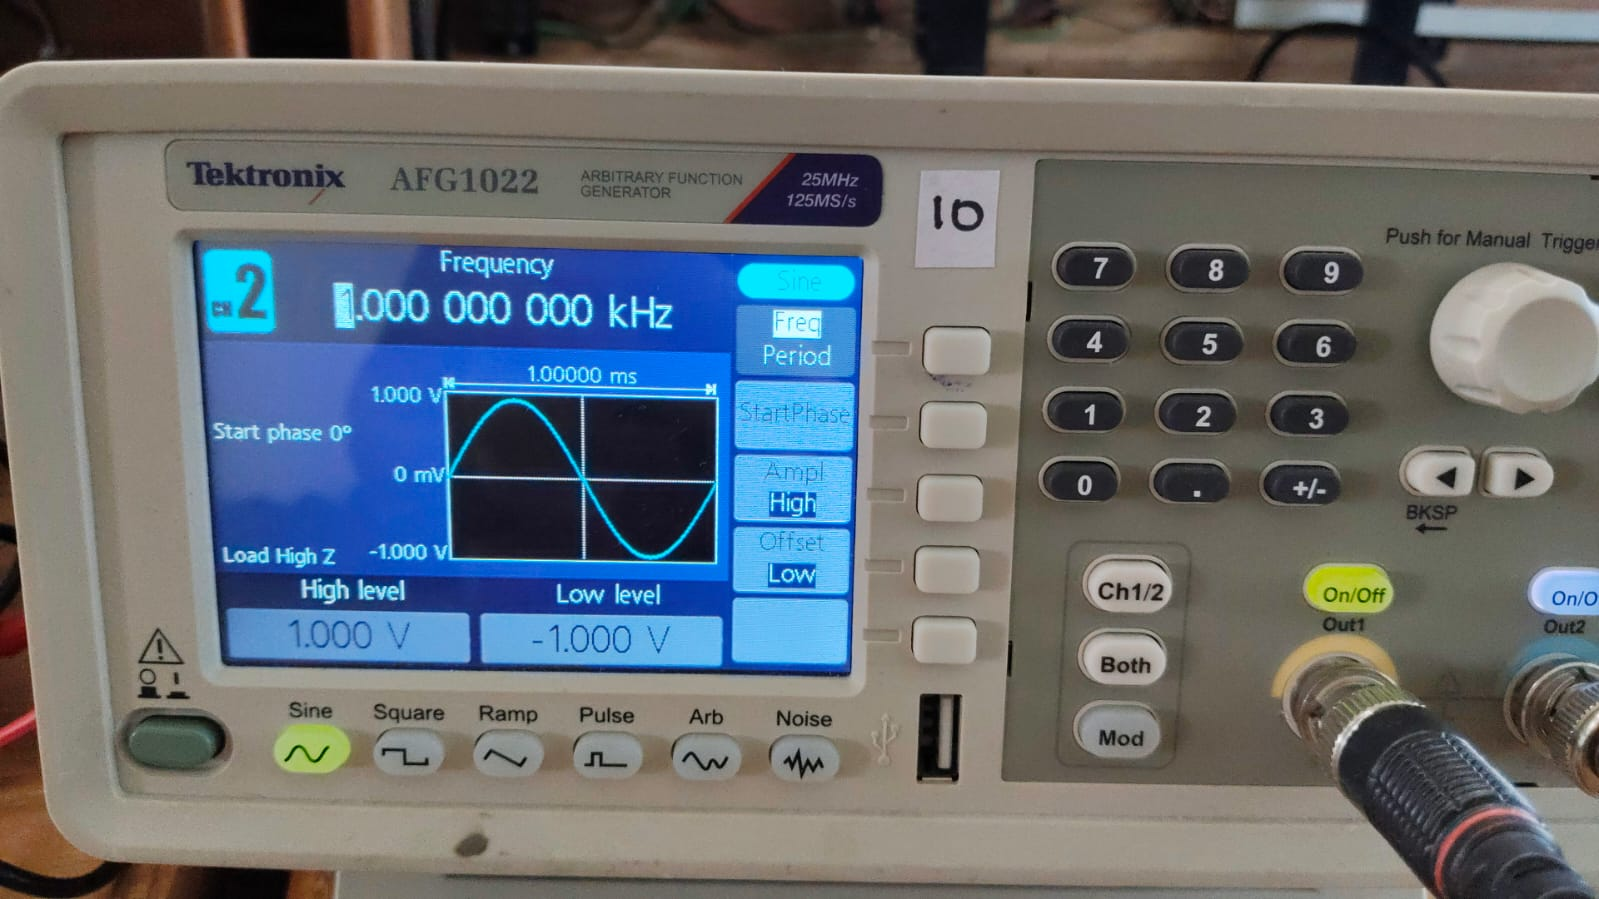
\includegraphics[width=0.45\textwidth]{figs/hpf_input_less_cutoff_1.jpeg}
    }
\end{figure}
\begin{figure}[H]
    \centering
    \subfigure[]{
        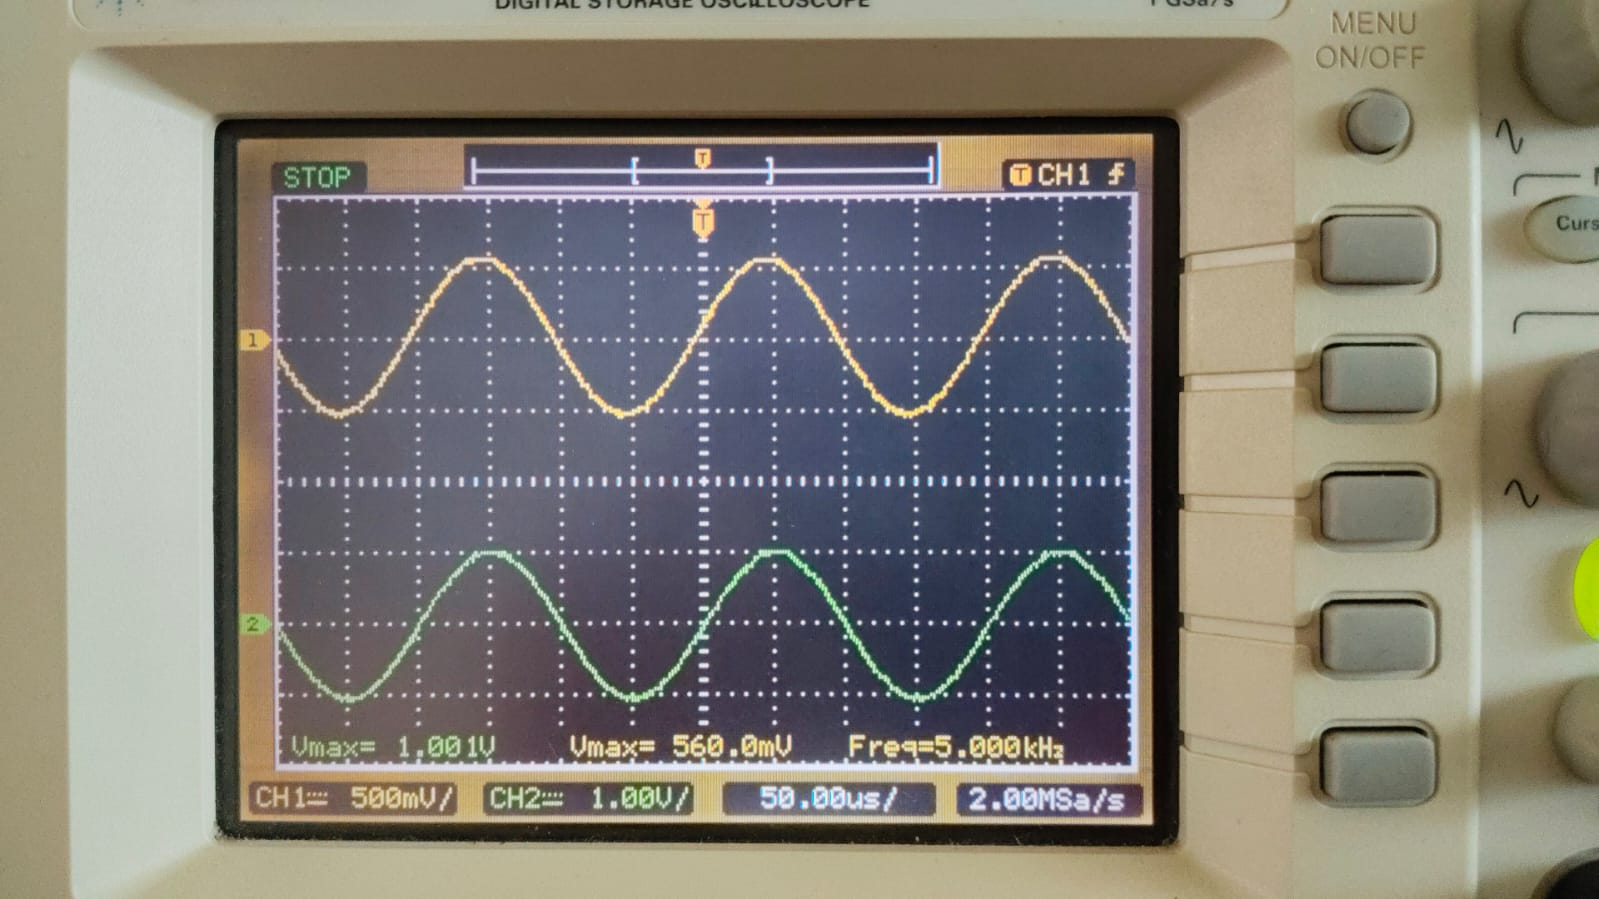
\includegraphics[width=0.45\textwidth]{figs/hpf_less_cutoff_2.jpeg}
    }
    \hfill
    \subfigure[]{
        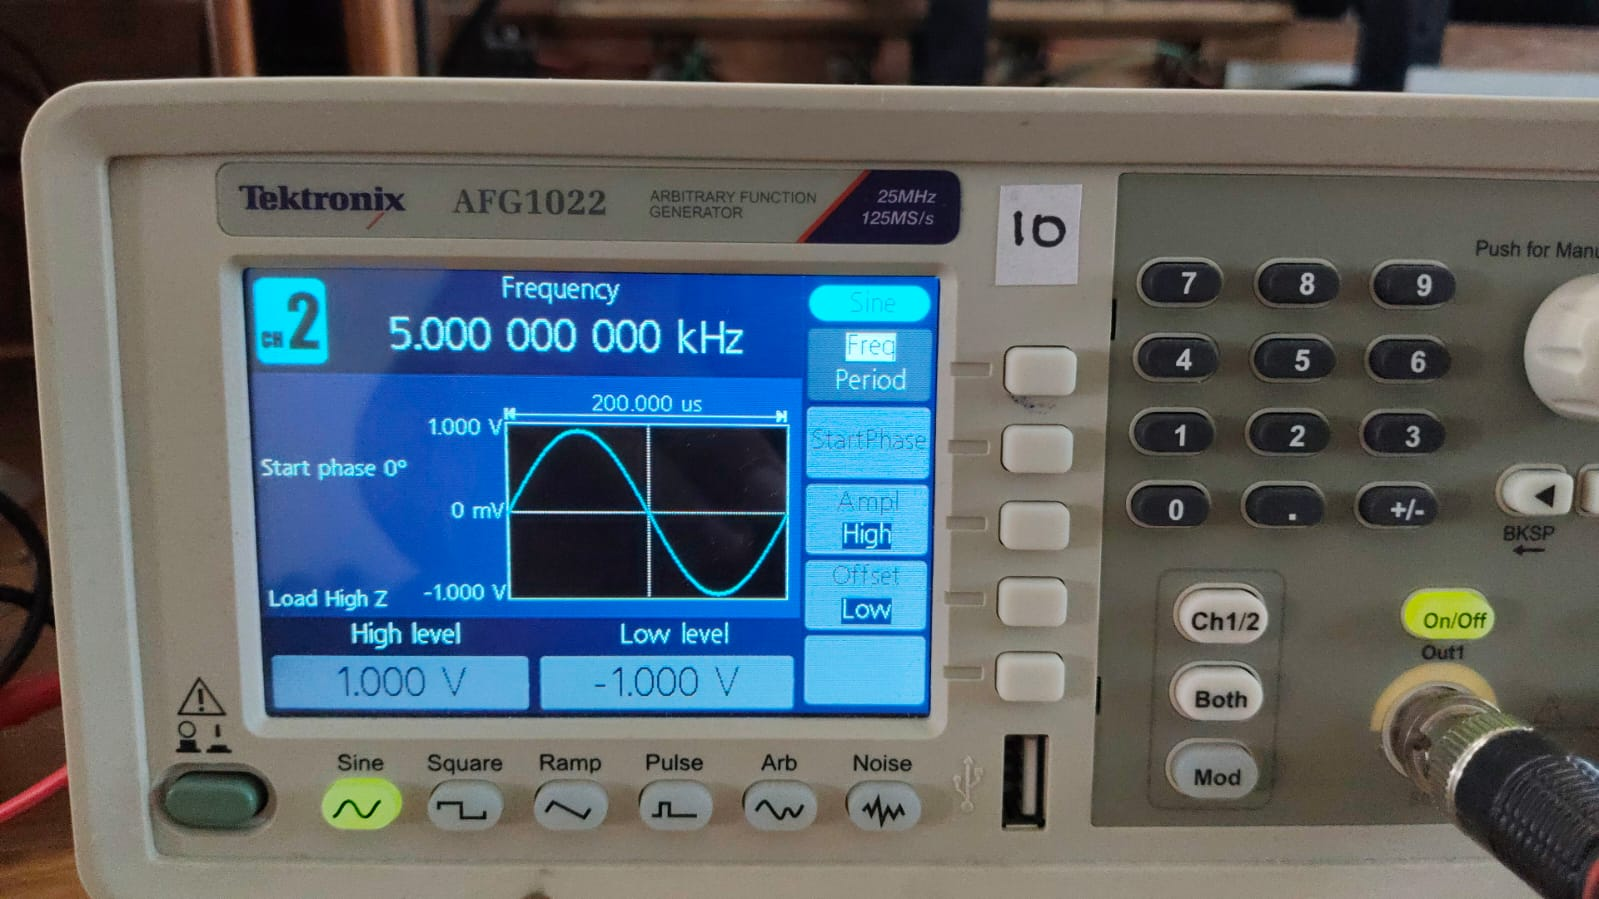
\includegraphics[width=0.45\textwidth]{figs/hpf_input_less_cutoff_2.jpeg}
    }
\end{figure}
\begin{figure}[H]
    \centering
    \subfigure[]{
        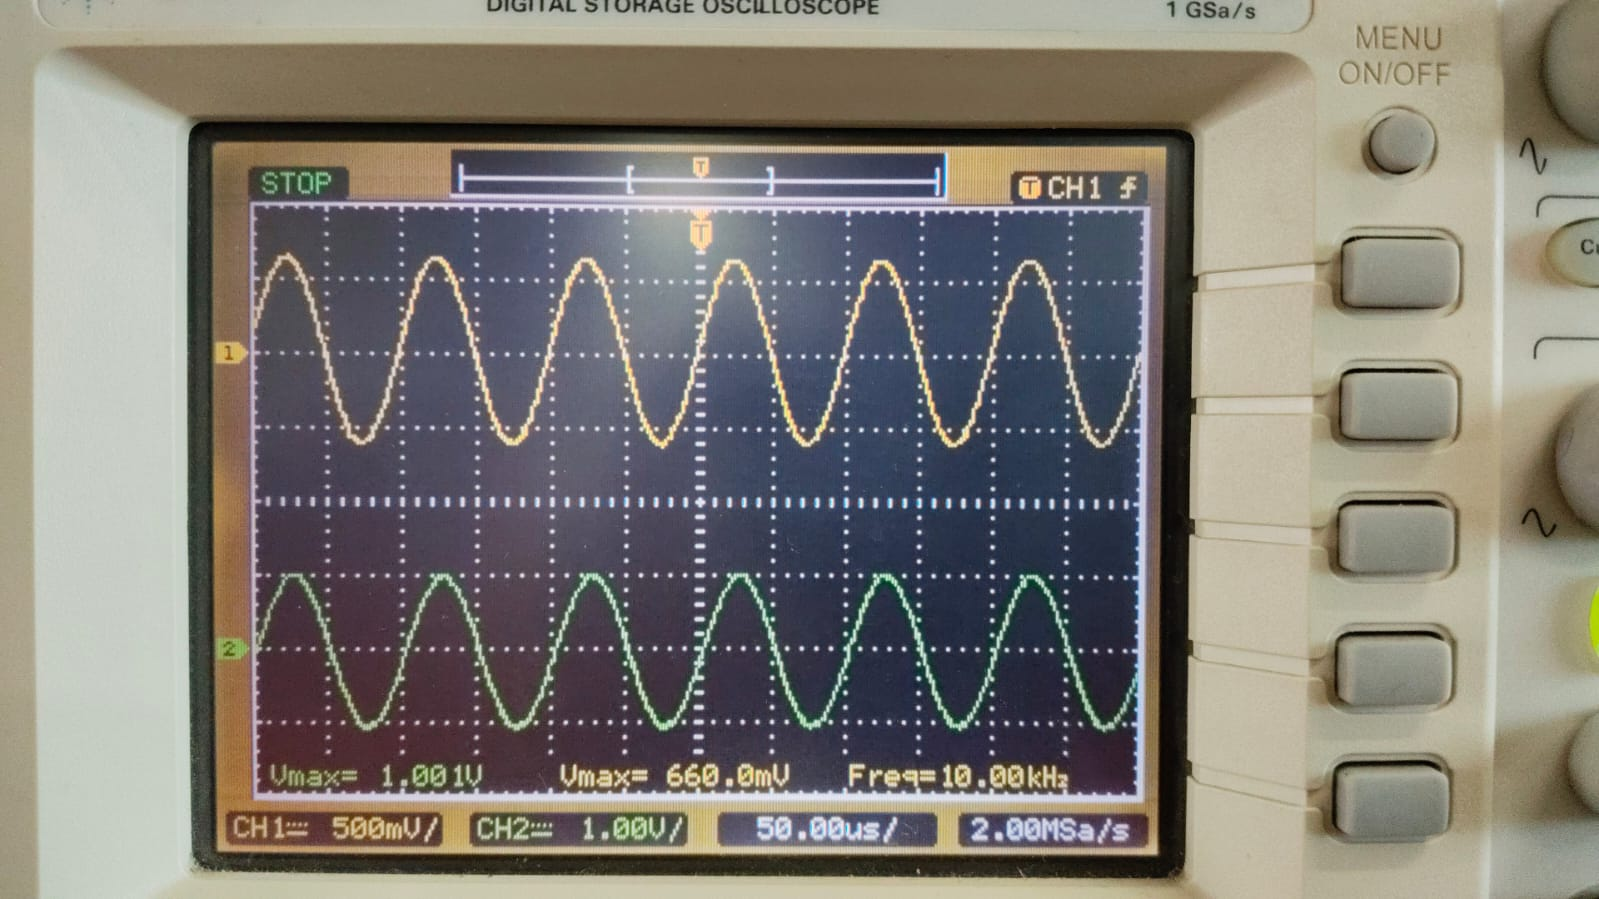
\includegraphics[width=0.45\textwidth]{figs/hpf_cutoff.jpeg}
    }
    \hfill
    \subfigure[]{
        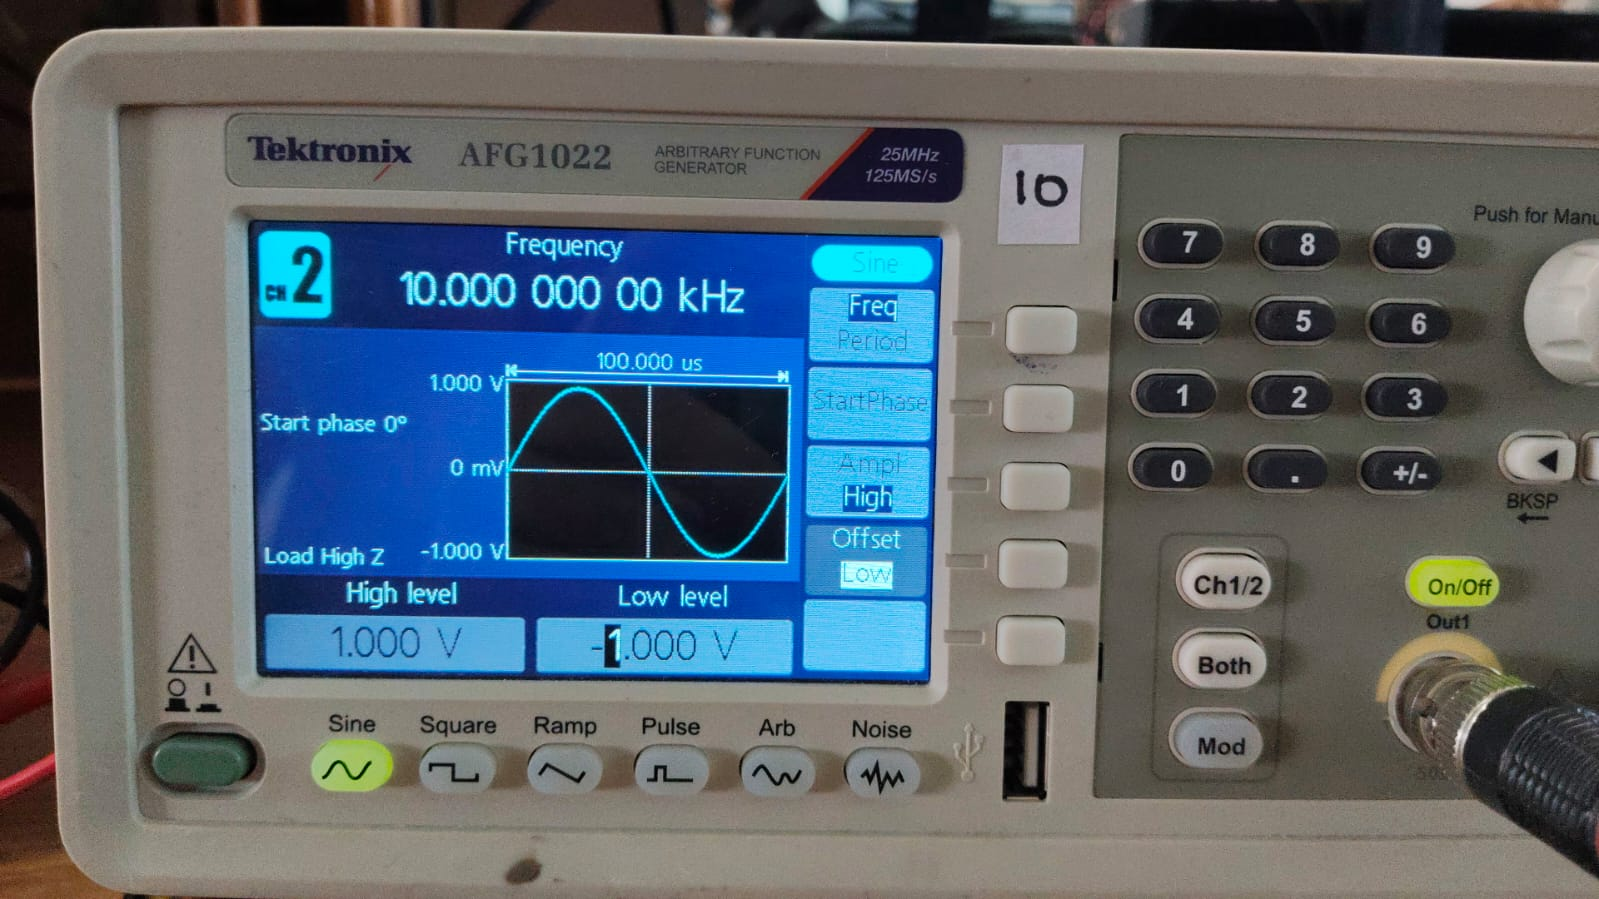
\includegraphics[width=0.45\textwidth]{figs/hpf_input_cutoff.jpeg}
    }
\end{figure}
\begin{figure}[H]
    \centering
    \subfigure[]{
        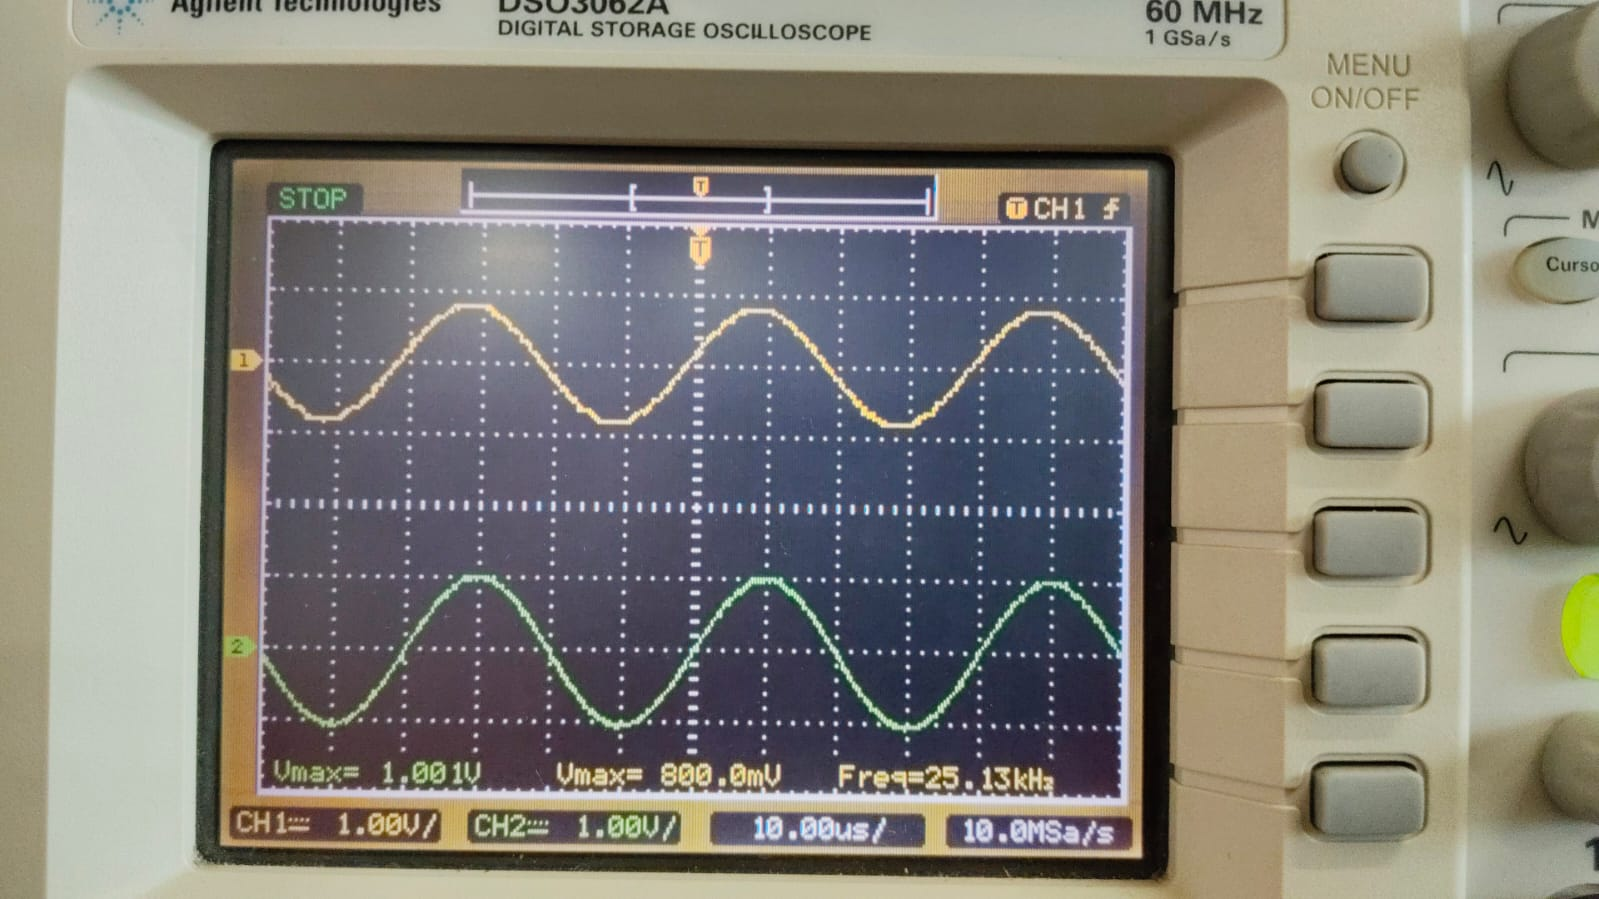
\includegraphics[width=0.45\textwidth]{figs/hpf_more_cutoff_1.jpeg}
    }
    \hfill
    \subfigure[]{
        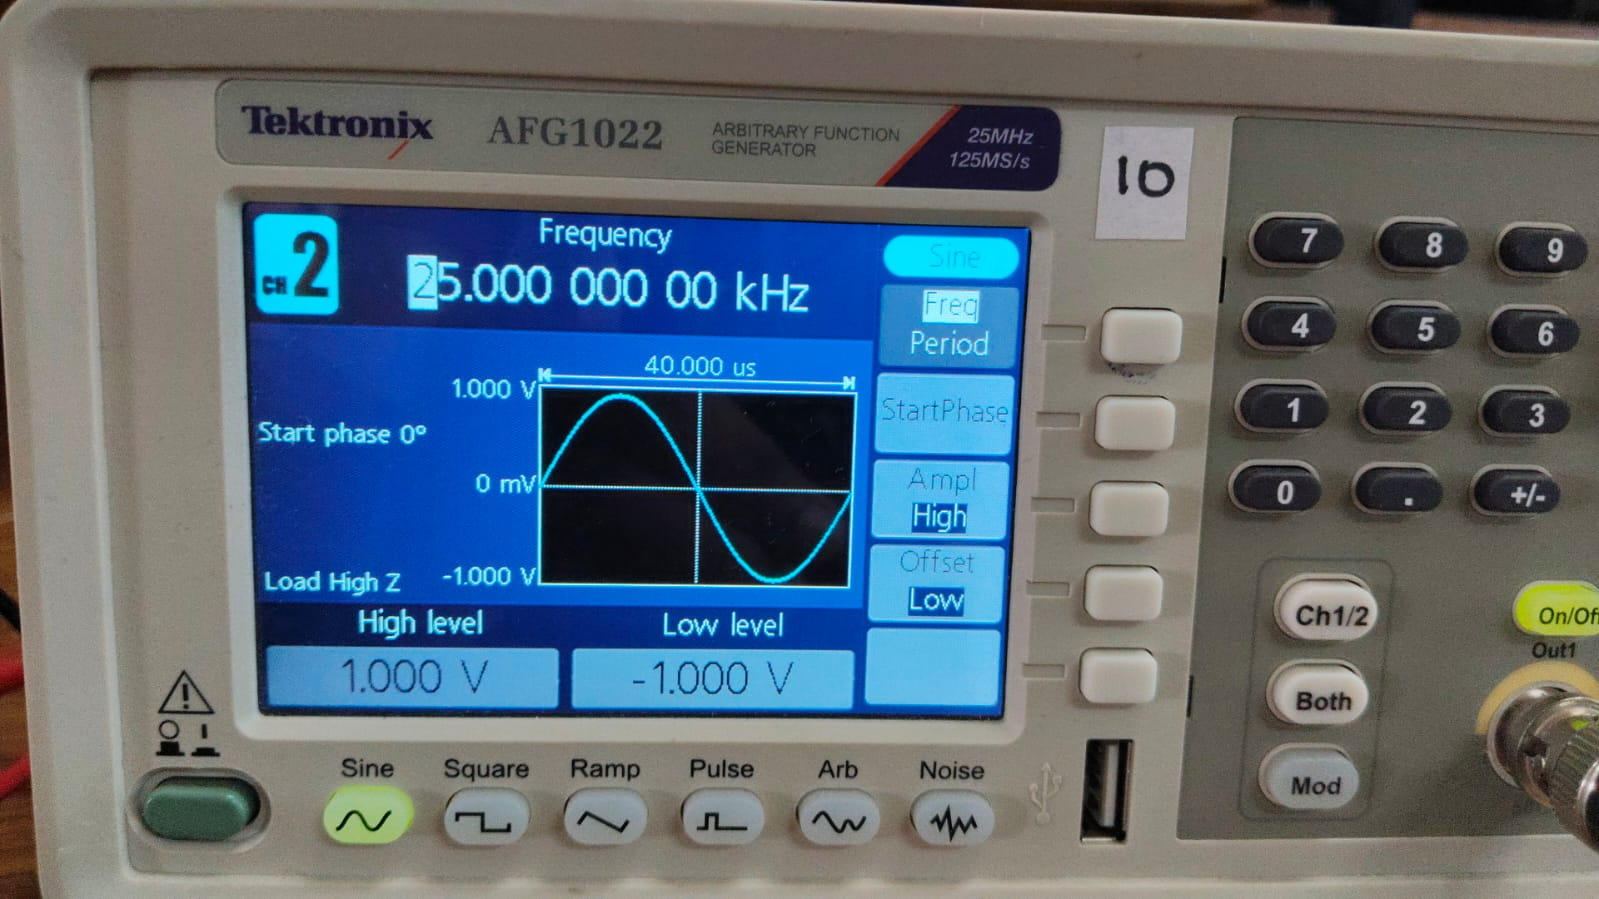
\includegraphics[width=0.45\textwidth]{figs/hpf_input_more_cutoff_1.jpeg}
    }
\end{figure}
\begin{figure}[H]
    \centering
    \subfigure[]{
        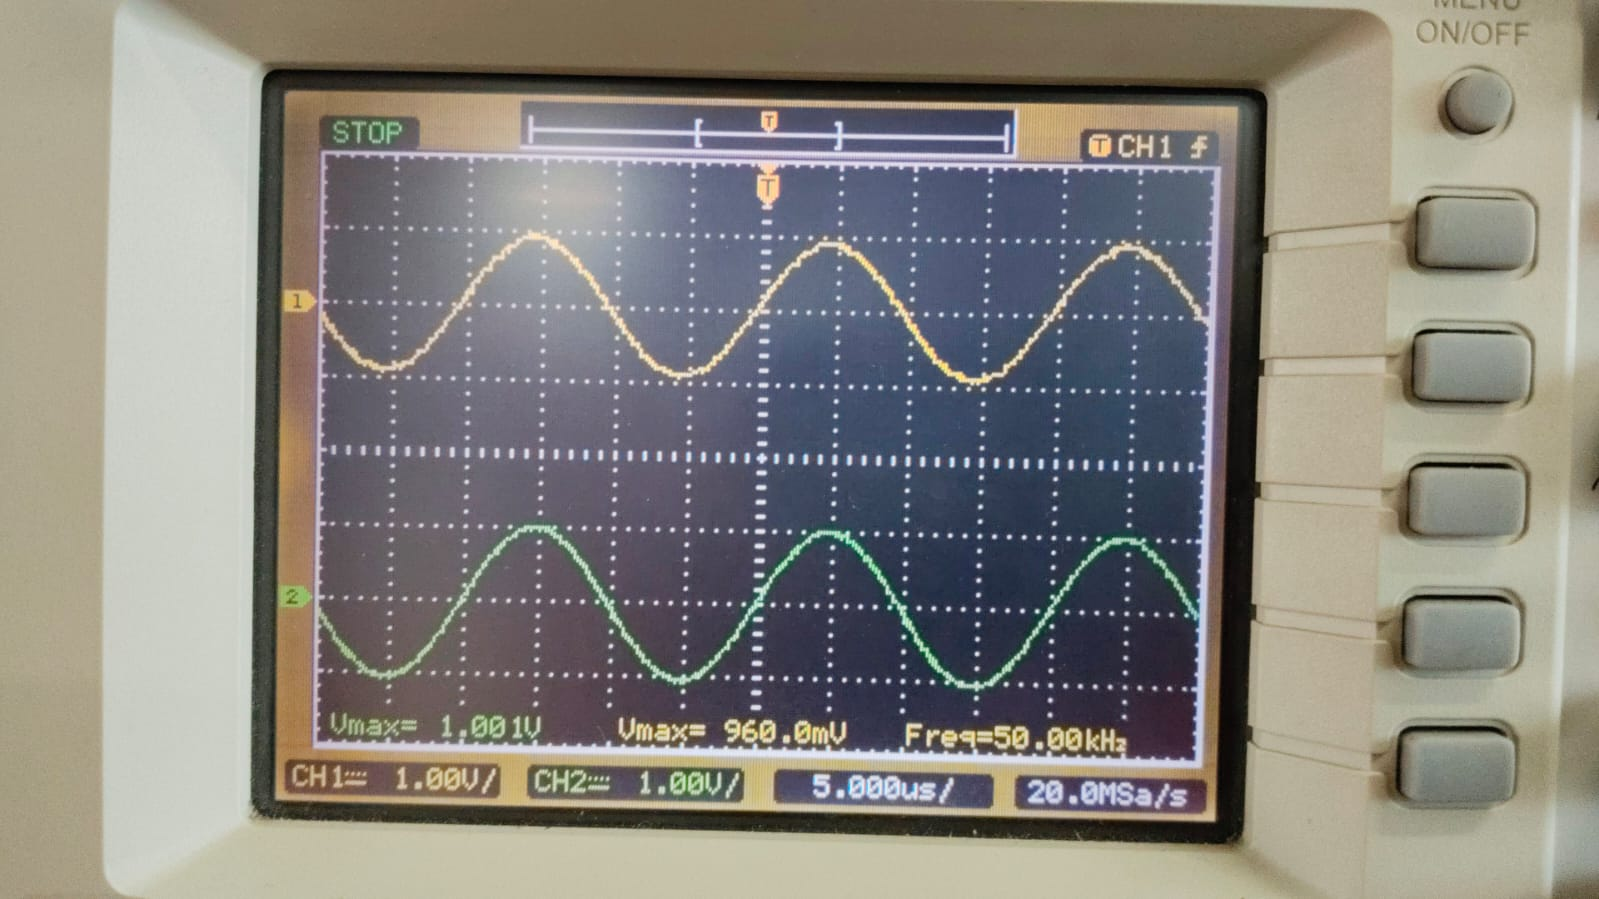
\includegraphics[width=0.45\textwidth]{figs/hpf_more_cutoff_2.jpeg}
    }
    \hfill
    \subfigure[]{
        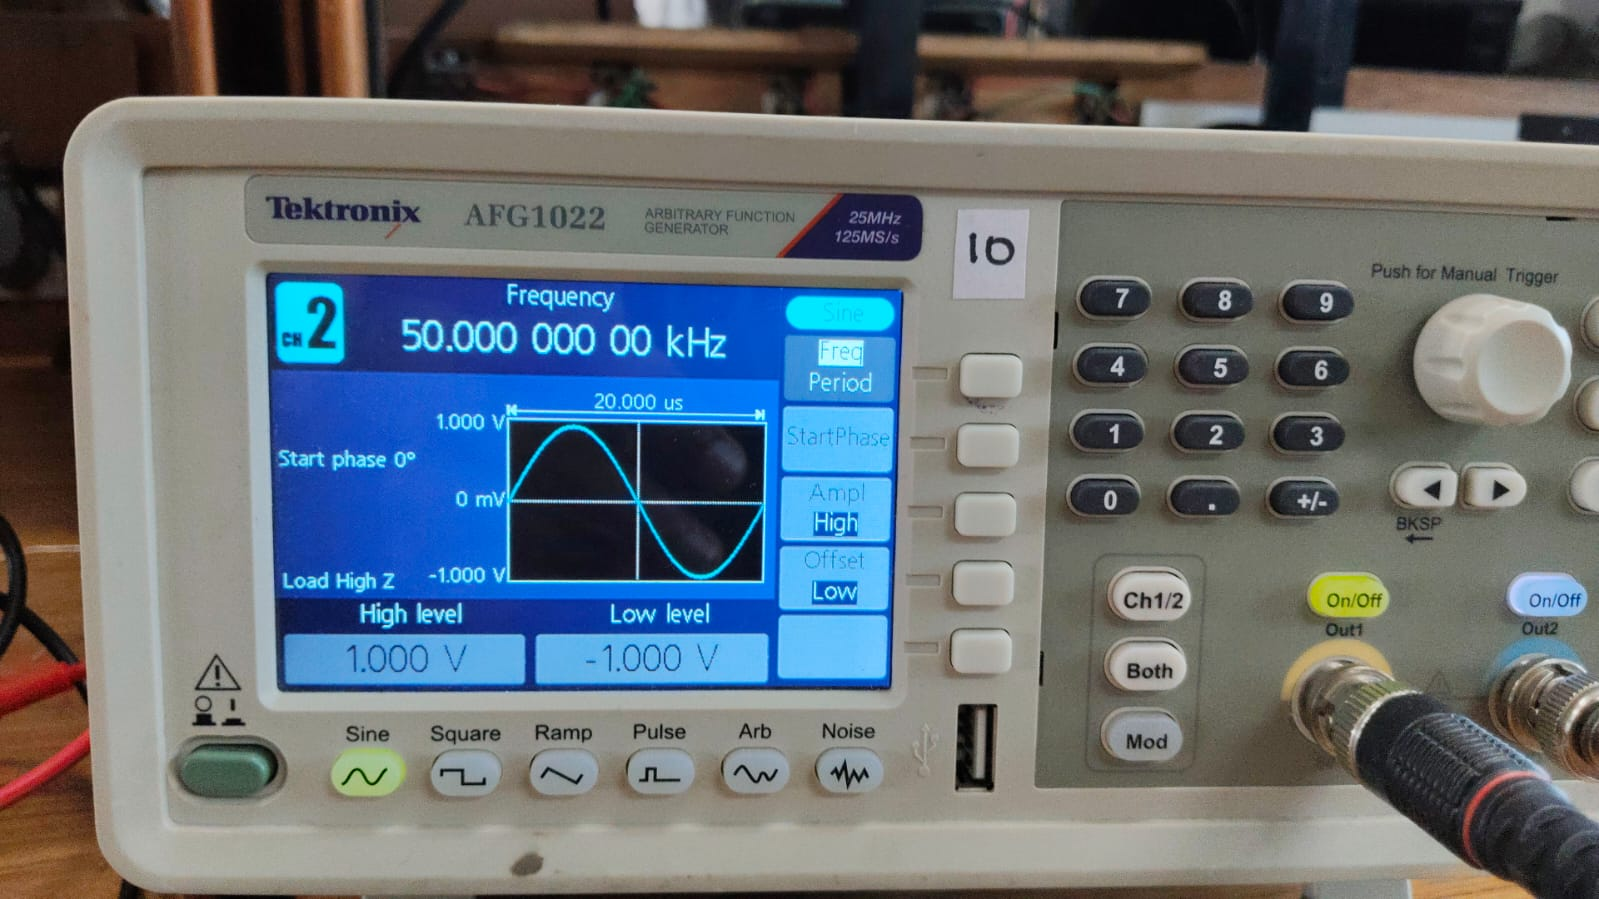
\includegraphics[width=0.45\textwidth]{figs/hpf_input_more_cutoff_2.jpeg}
    }
\end{figure}
\begin{figure}[H]
    \centering
    \subfigure[]{
        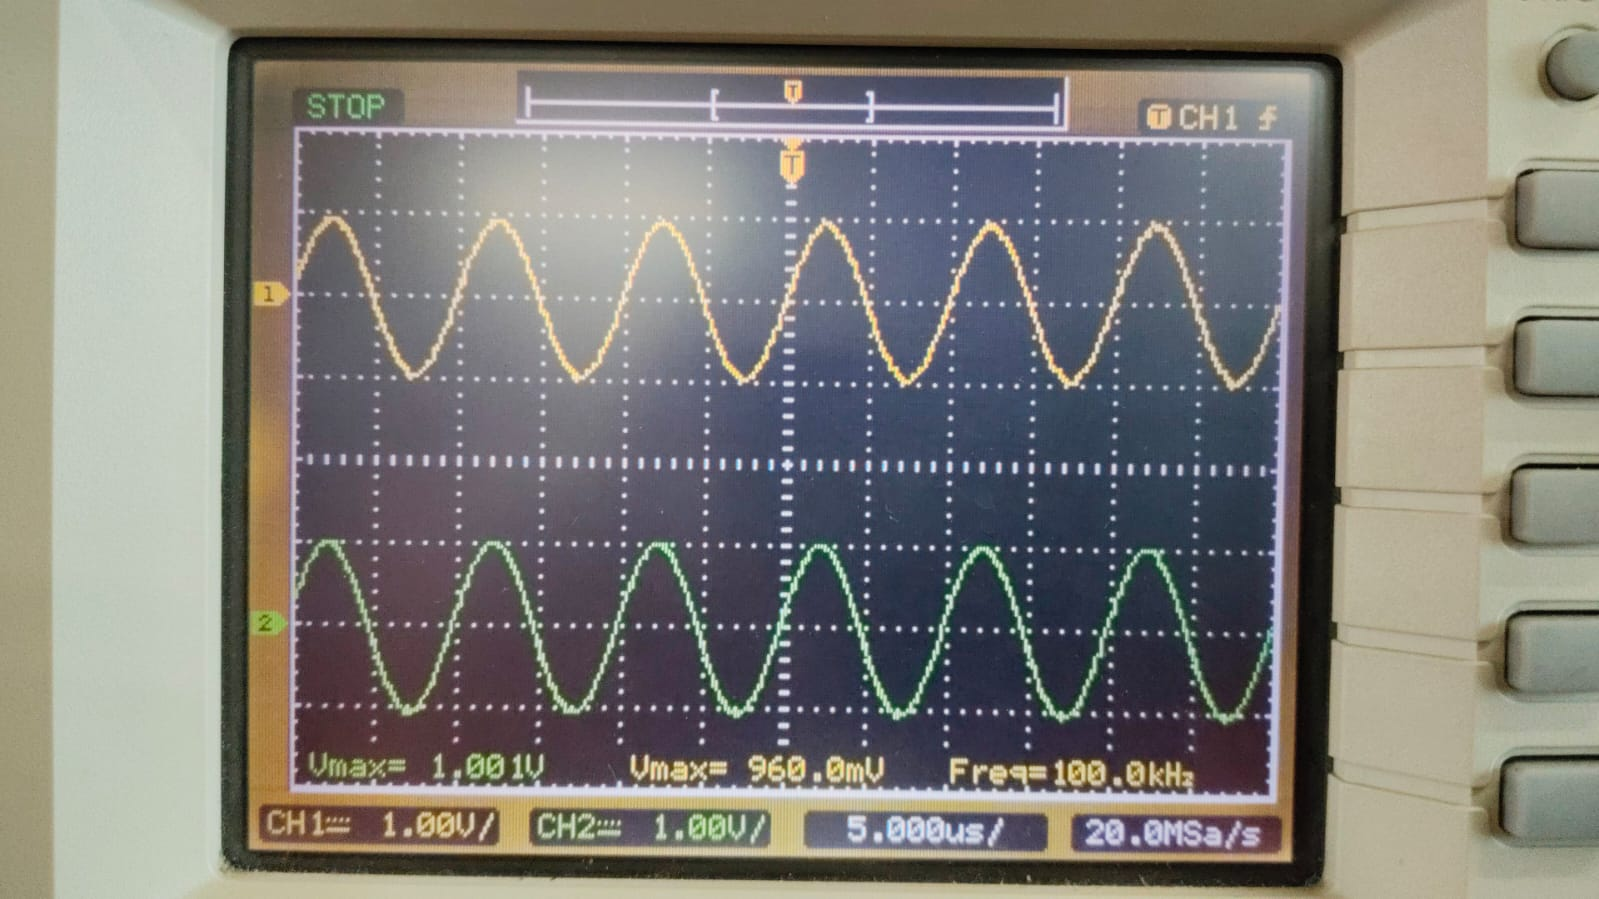
\includegraphics[width=0.45\textwidth]{figs/hpf_more_cutoff_3.jpeg}
    }
    \hfill
    \subfigure[]{
        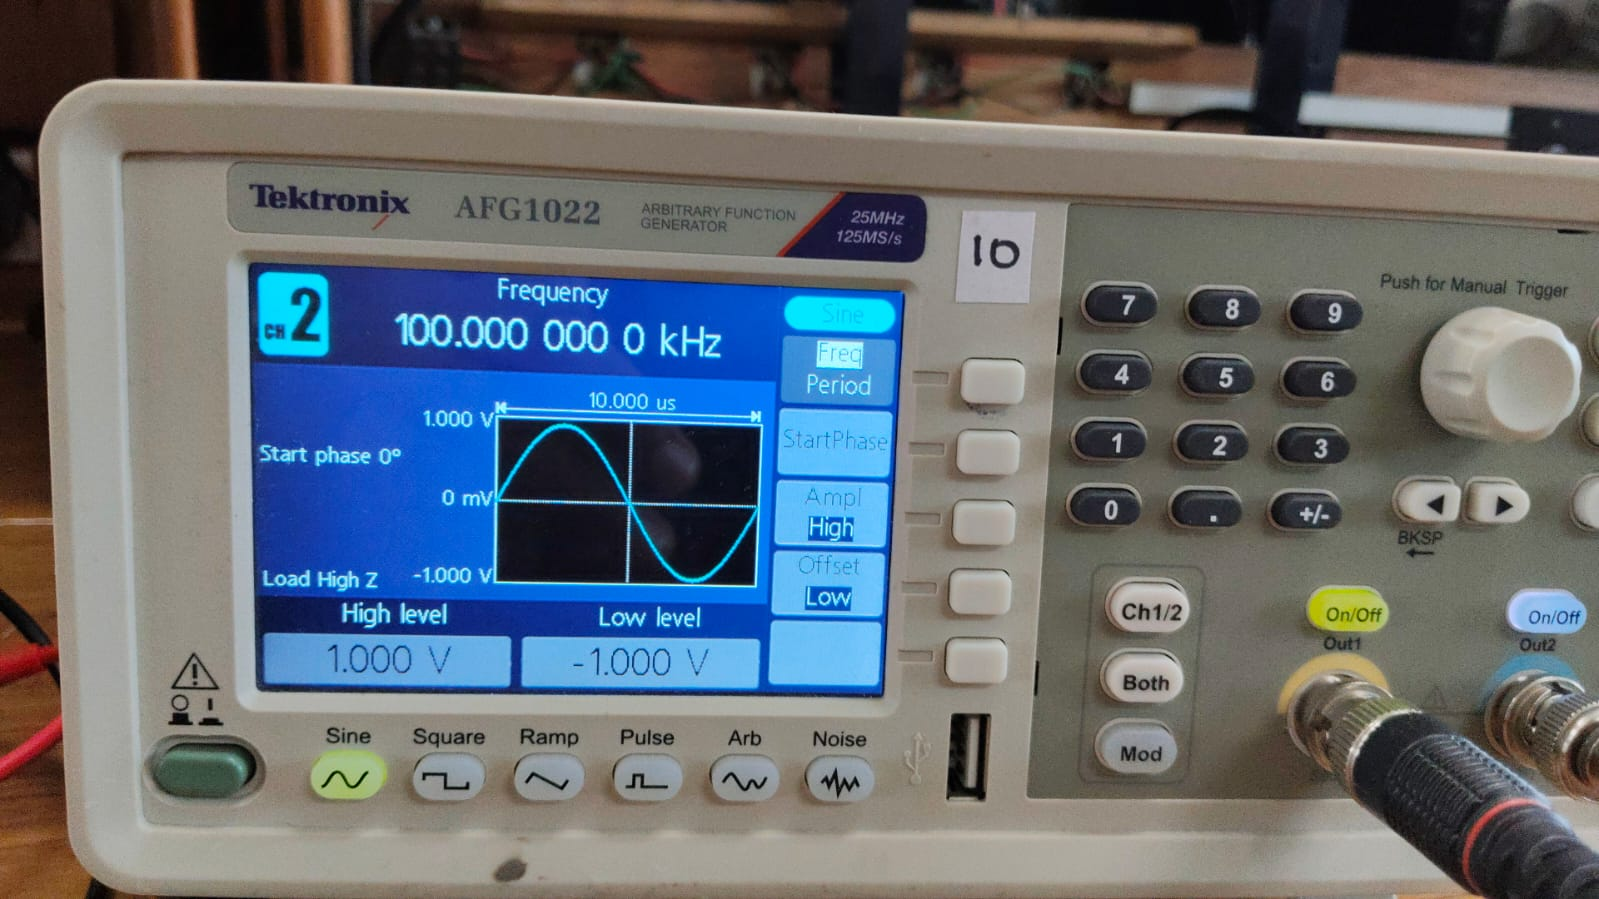
\includegraphics[width=0.45\textwidth]{figs/hpf_input_more_cutoff_3.jpeg}
    }
\end{figure}
\begin{figure}[H]
    \centering
    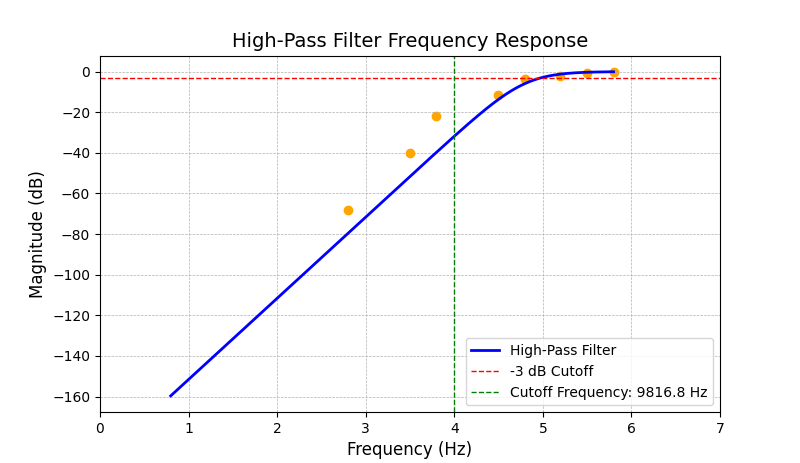
\includegraphics[width=\textwidth]{figs/high.png}
    \caption{Bode plot for HPF}
\end{figure}

\subsection{Low Pass Filter (LPF) Design}
A low pass filter allows signals with frequencies lower than a certain cutoff frequency to pass while attenuating higher frequencies. The cutoff frequency $f_{c2}$ is given by:
\begin{equation}
    f_{c2} = \frac{1}{2\pi \sqrt{R_3 R_4 C_3 C_4}}
\end{equation}
This filter is useful in applications where high-frequency noise needs to be removed, such as in audio processing and communication systems.\\
\textbf{The values of Resistors are:} 8.2kohm, 8.2kohm\\
\textbf{The values of Capacitors in LPF part are:} 1nF, 1nF \\
\begin{figure}[H]
    \centering
    \subfigure[]{
        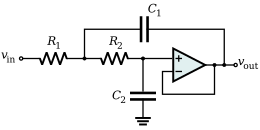
\includegraphics[width=0.45\textwidth]{figs/lowpass.png}
    }
    \hfill
    \subfigure[]{
        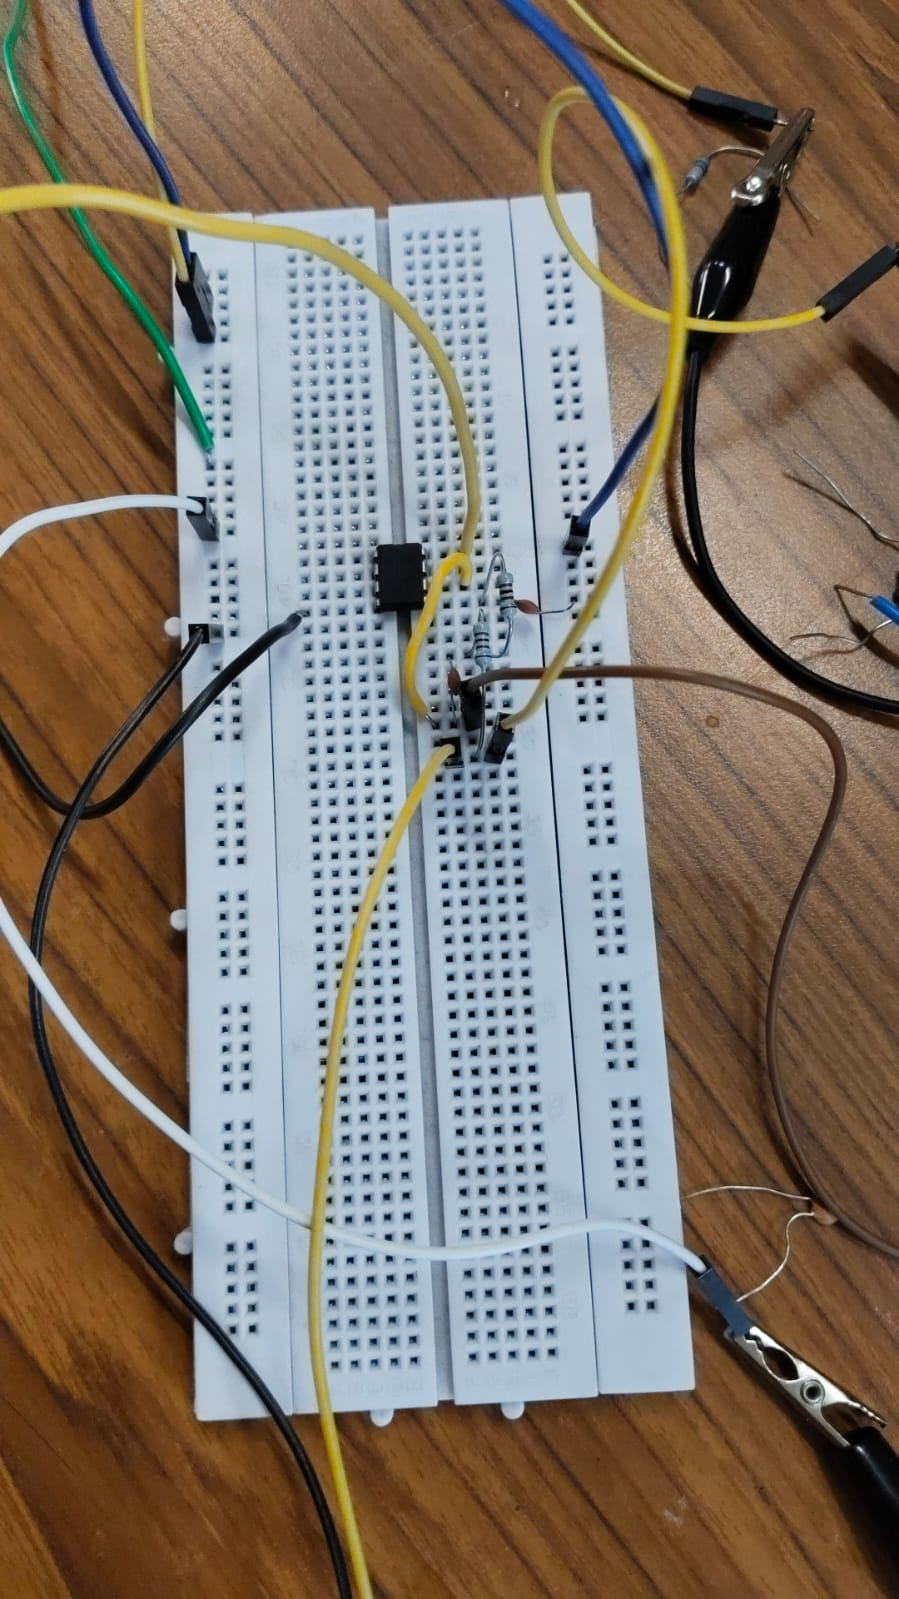
\includegraphics[width=0.45\textwidth]{figs/lpf_circuit.jpeg}
    }
\end{figure}
\begin{table}[H]
    \centering
    \renewcommand{\arraystretch}{1.3} % Adjust row height
    \begin{tabular}{|c|c|c|}
        \hline
        \textbf{S. No.} & \textbf{Input Frequency (Hz)} &\textbf{Output Voltage (V)} \\
        \hline
        1 & 1000 & 1  \\
        2 & 5000 & 0.88  \\
        3 & 10000 & 0.8  \\
        4 & 19000 & 0.64  \\
        5 & 20000 & 0.64  \\
        6 & 50000 & 0.52  \\
        7 & 100000 & 0.48  \\
        \hline
    \end{tabular}
    \caption{Observation Table for Frequency Response for LPF}
    \label{tab:observation}
\end{table}
\begin{figure}[H]
    \centering
    \subfigure[]{
        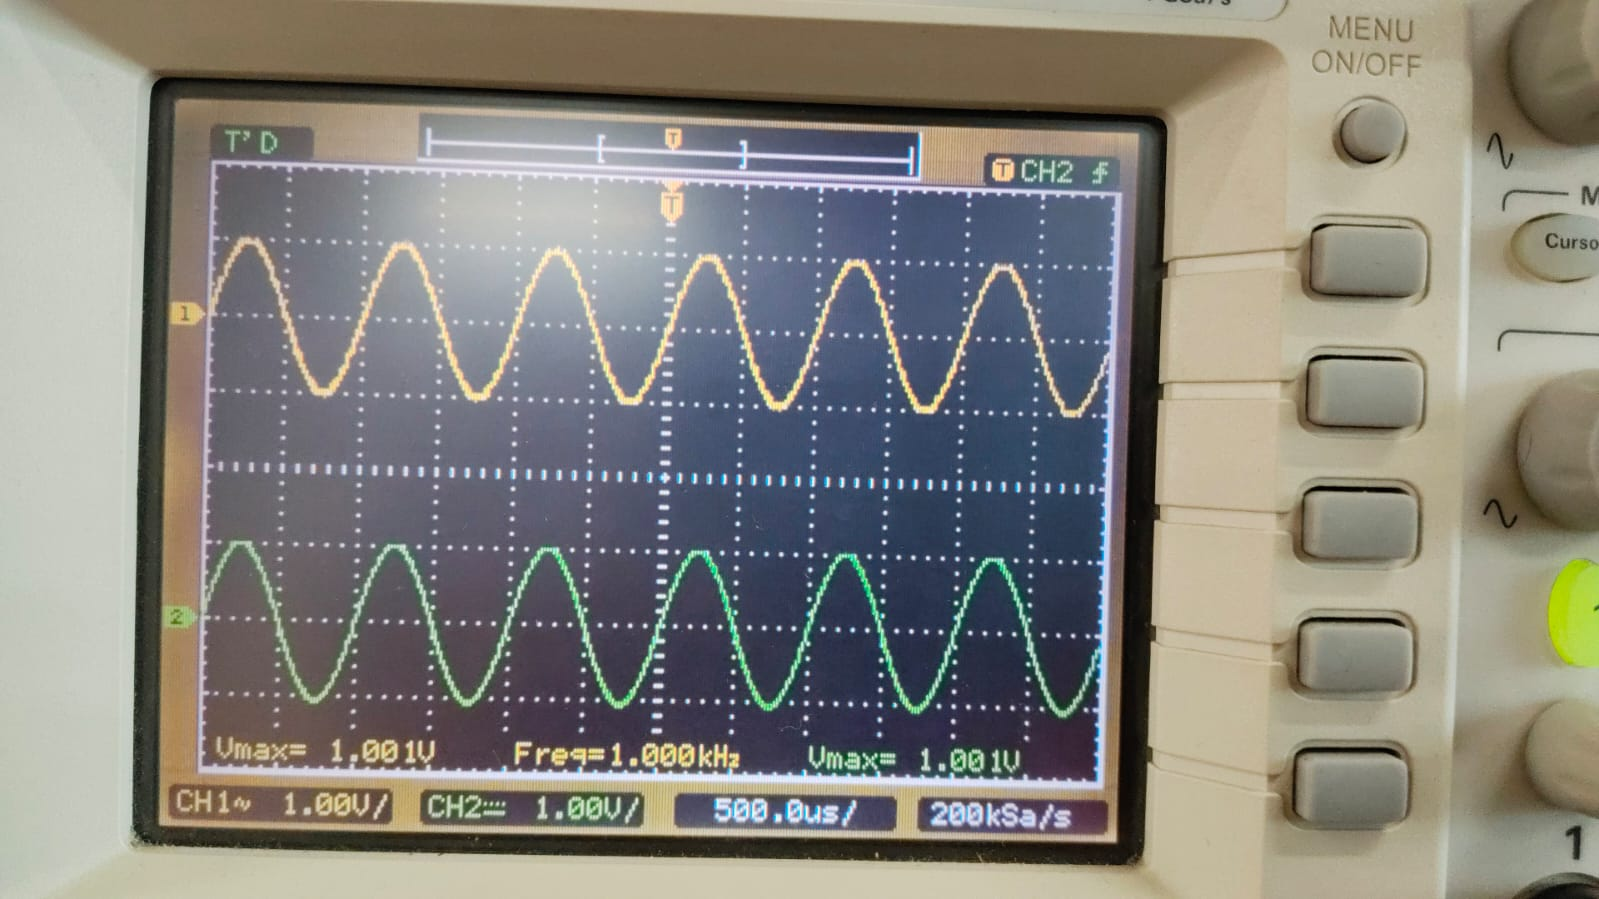
\includegraphics[width=0.45\textwidth]{figs/lpf_less_cutoff_3.jpeg}
    }
    \hfill
    \subfigure[]{
        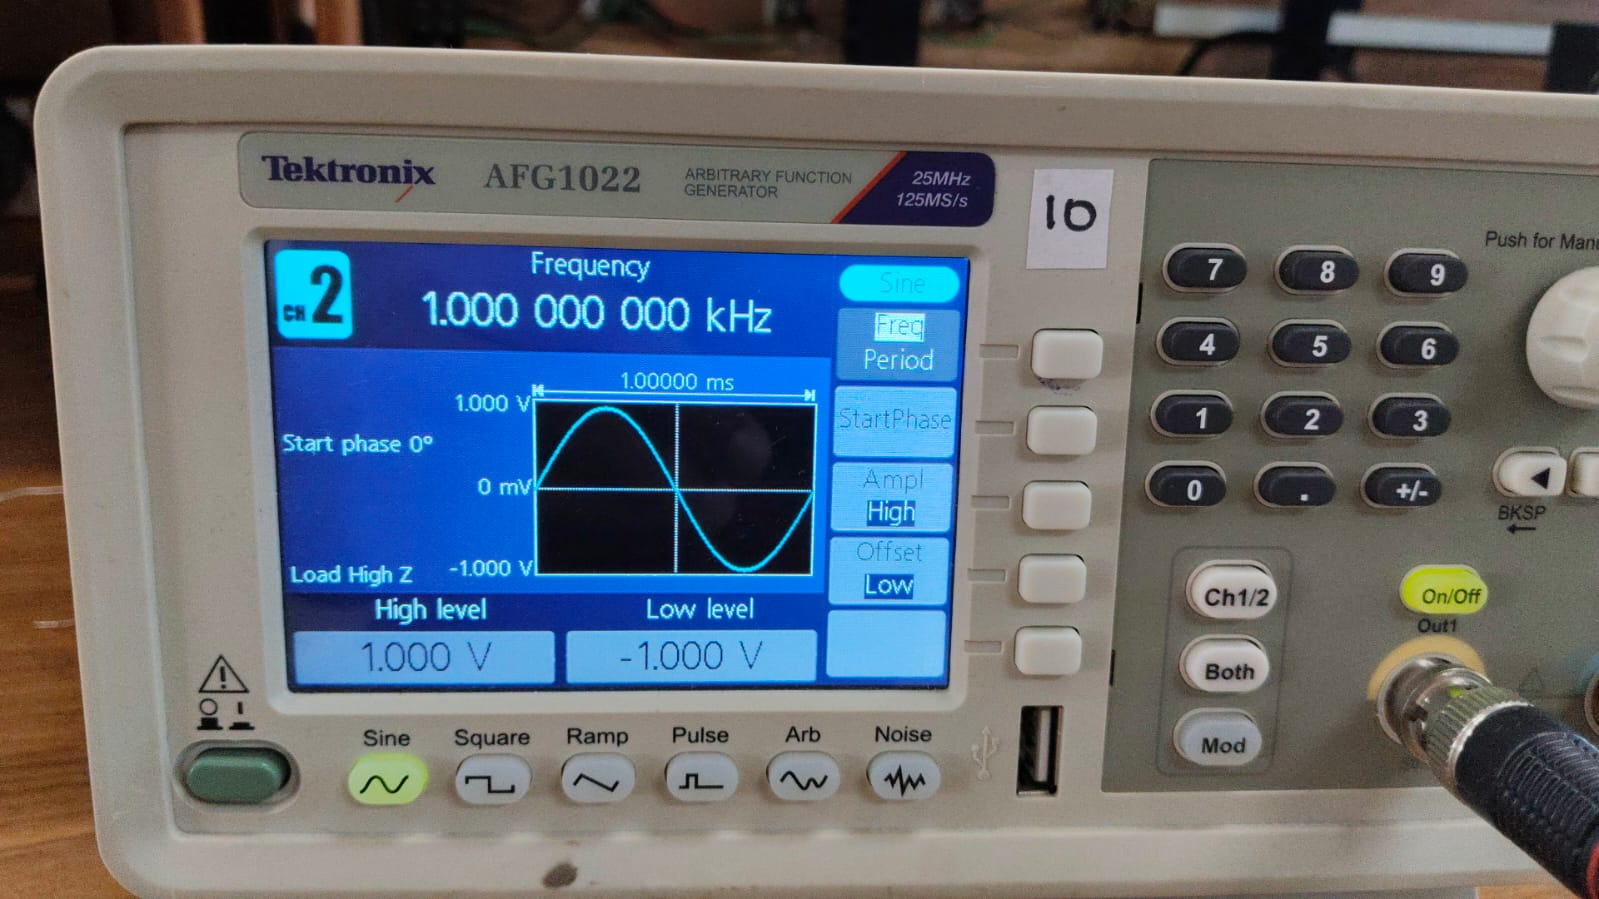
\includegraphics[width=0.45\textwidth]{figs/lpf_input_less_cutoff_3.jpeg}
    }
\end{figure}
\begin{figure}[H]
    \centering
    \subfigure[]{
        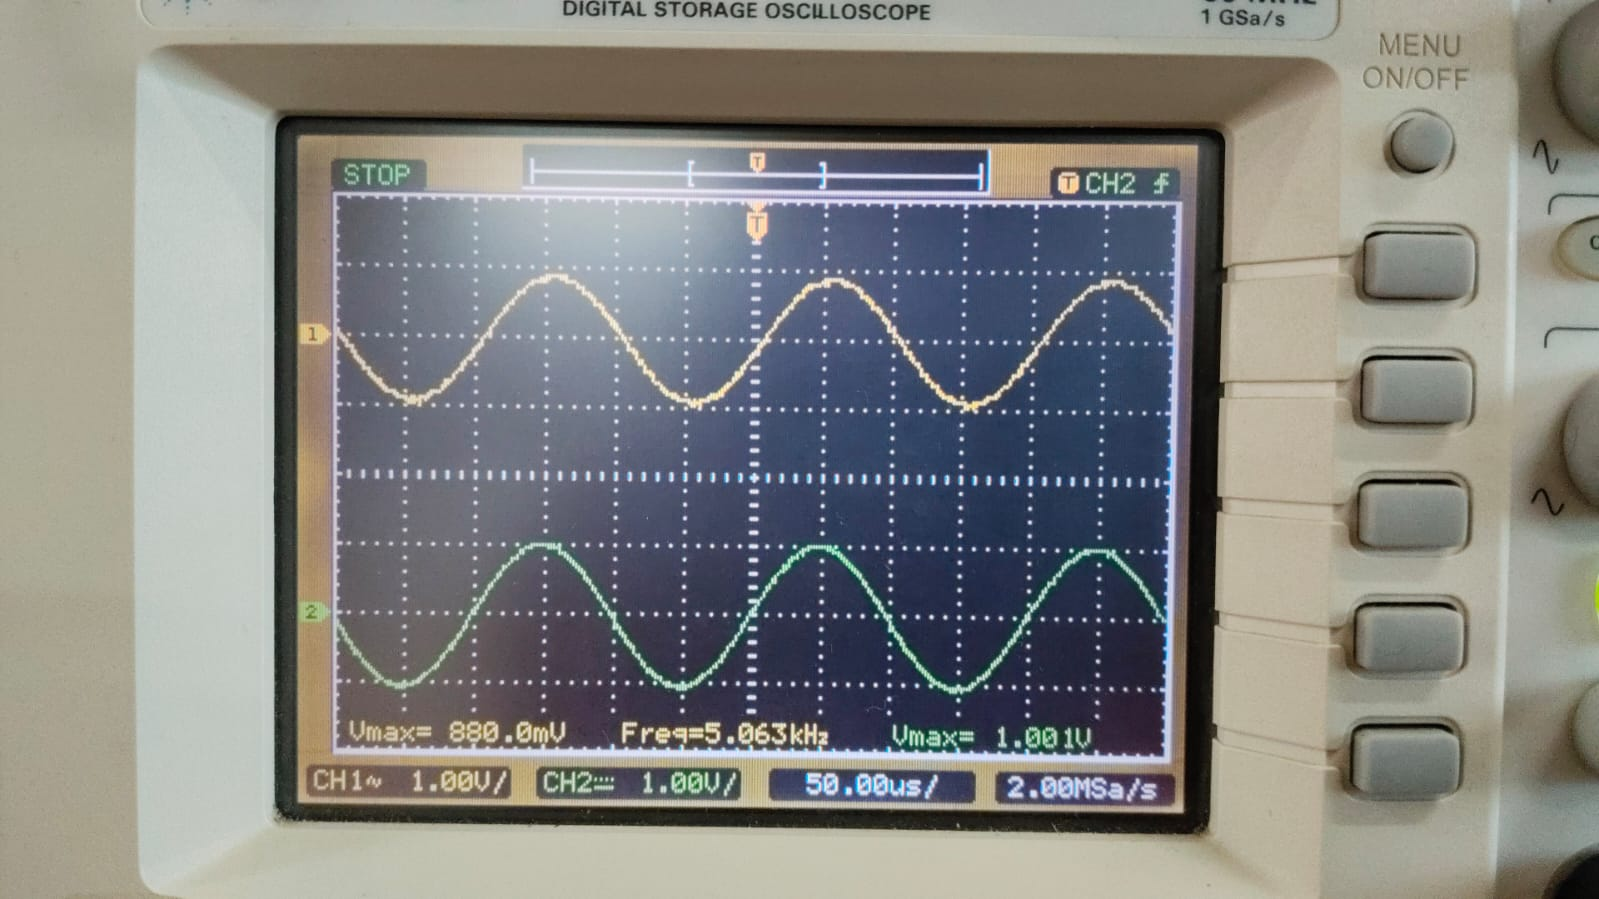
\includegraphics[width=0.45\textwidth]{figs/lpf_less_cutoff_2.jpeg}
    }
    \hfill
    \subfigure[]{
        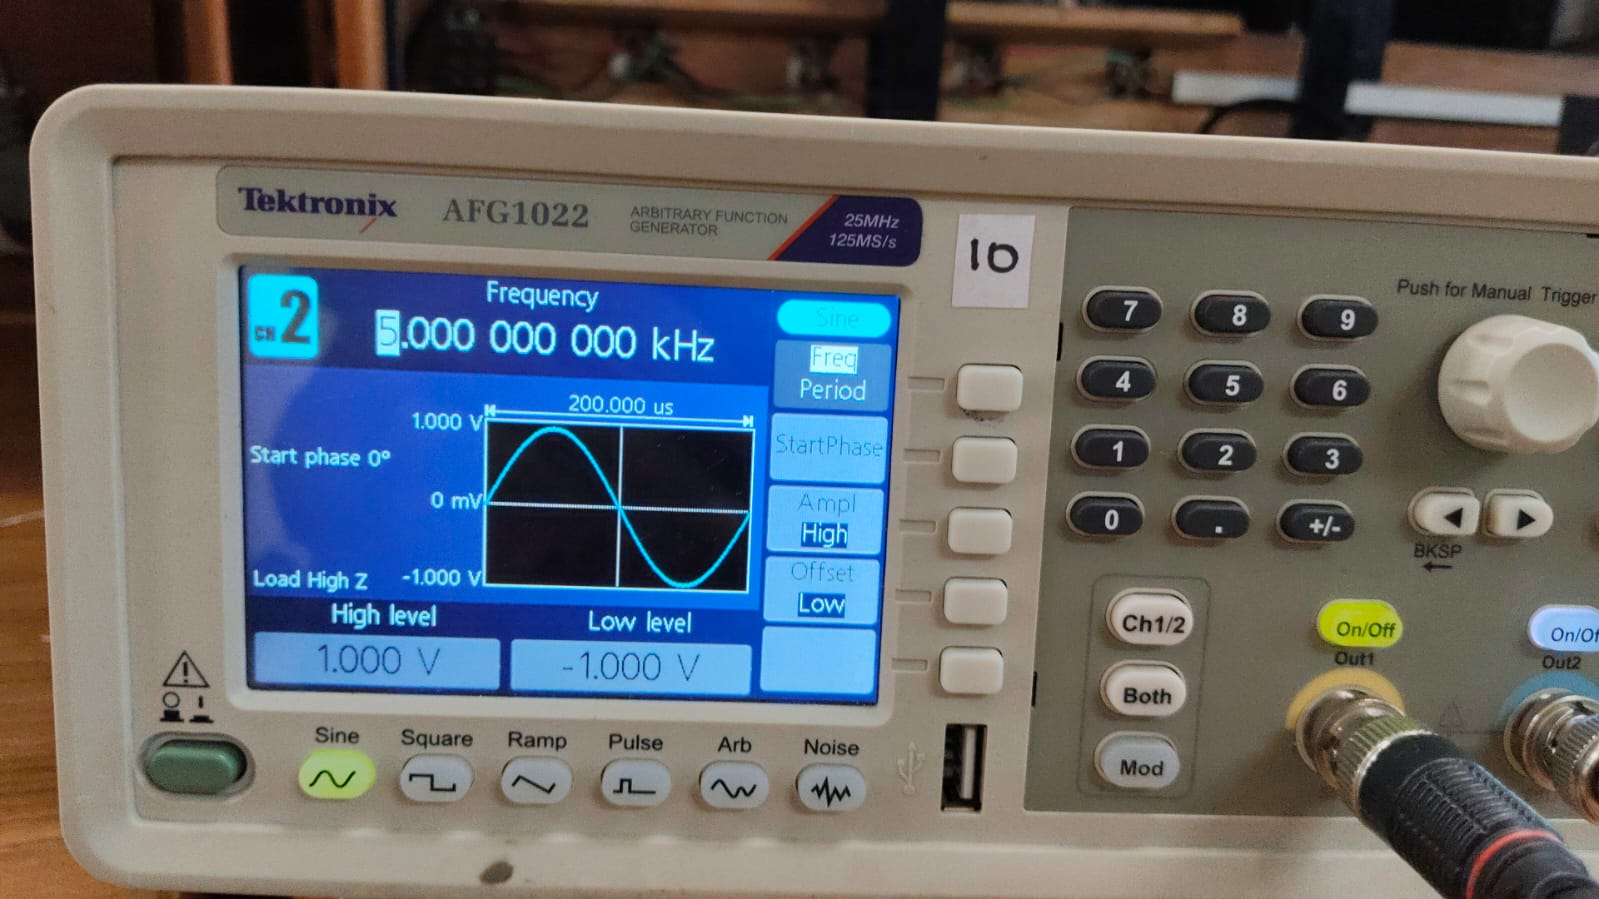
\includegraphics[width=0.45\textwidth]{figs/lpf_input_less_cutoff_2.jpeg}
    }
\end{figure}
\begin{figure}[H]
    \centering
    \subfigure[]{
        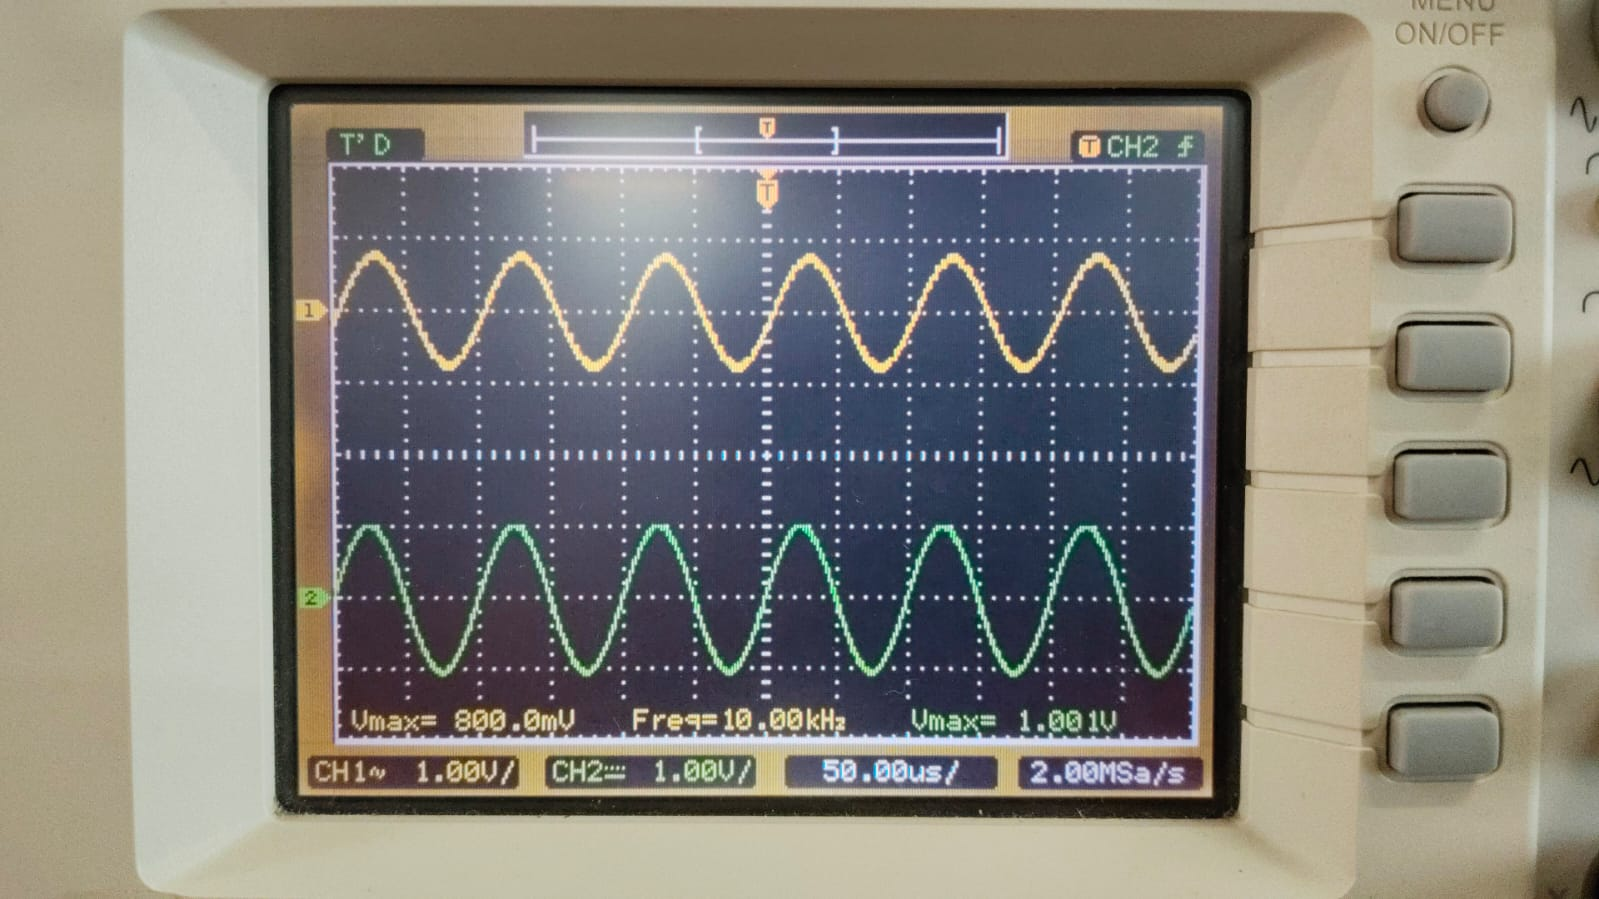
\includegraphics[width=0.45\textwidth]{figs/lpf_less_cutoff_1.jpeg}
    }
    \hfill
    \subfigure[]{
        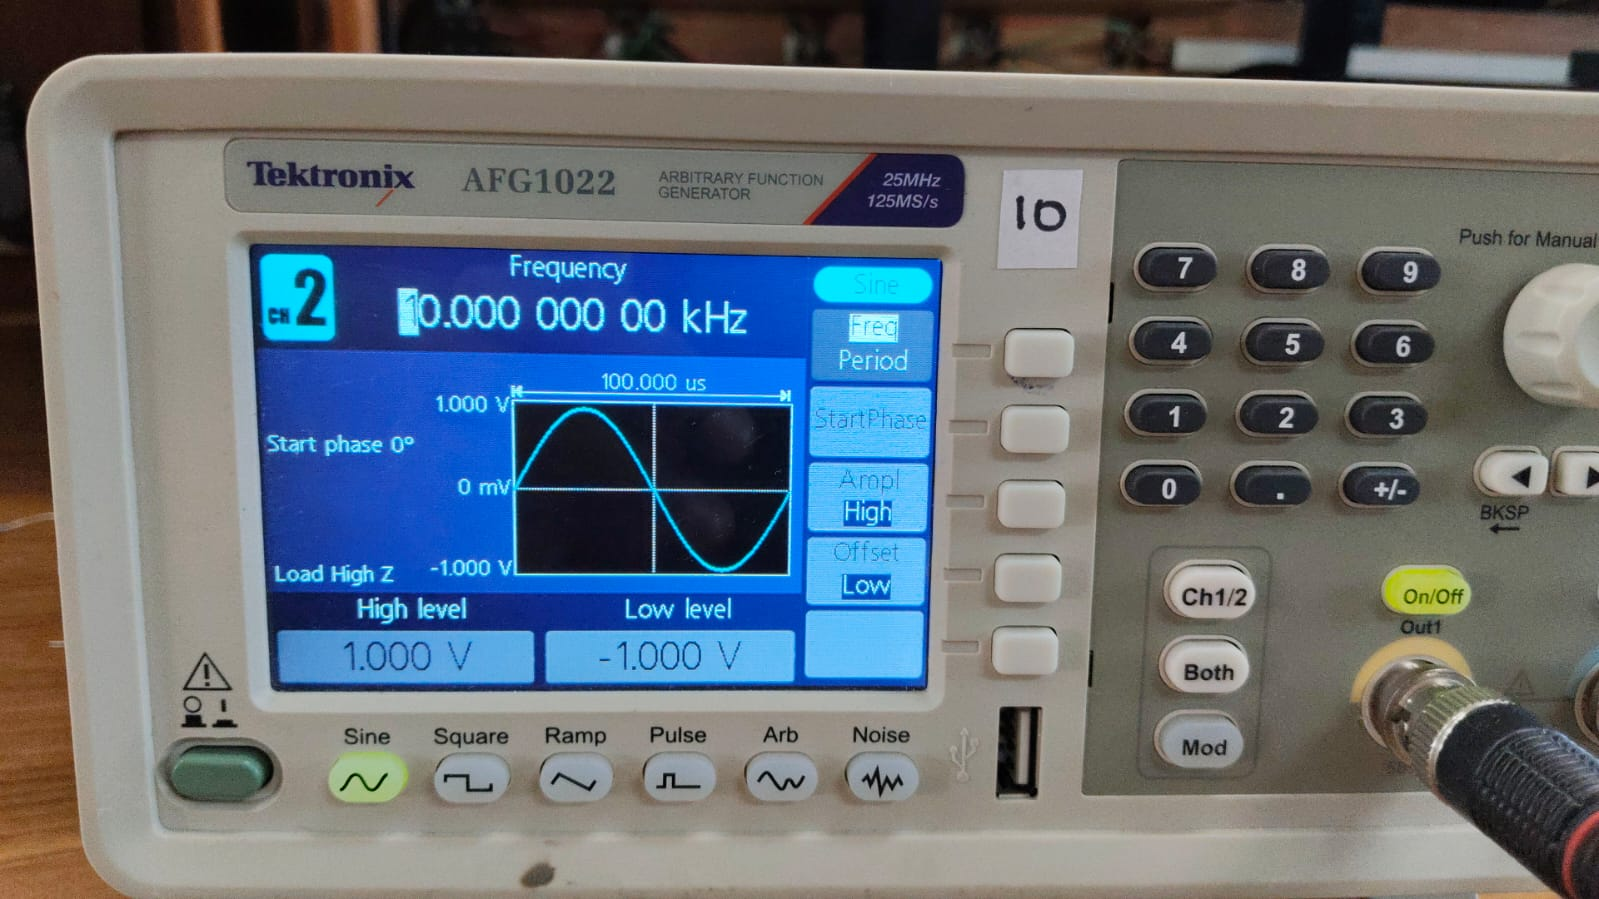
\includegraphics[width=0.45\textwidth]{figs/lpf_input_less_cutoff_1.jpeg}
    }
\end{figure}
\begin{figure}[H]
    \centering
    \subfigure[]{
        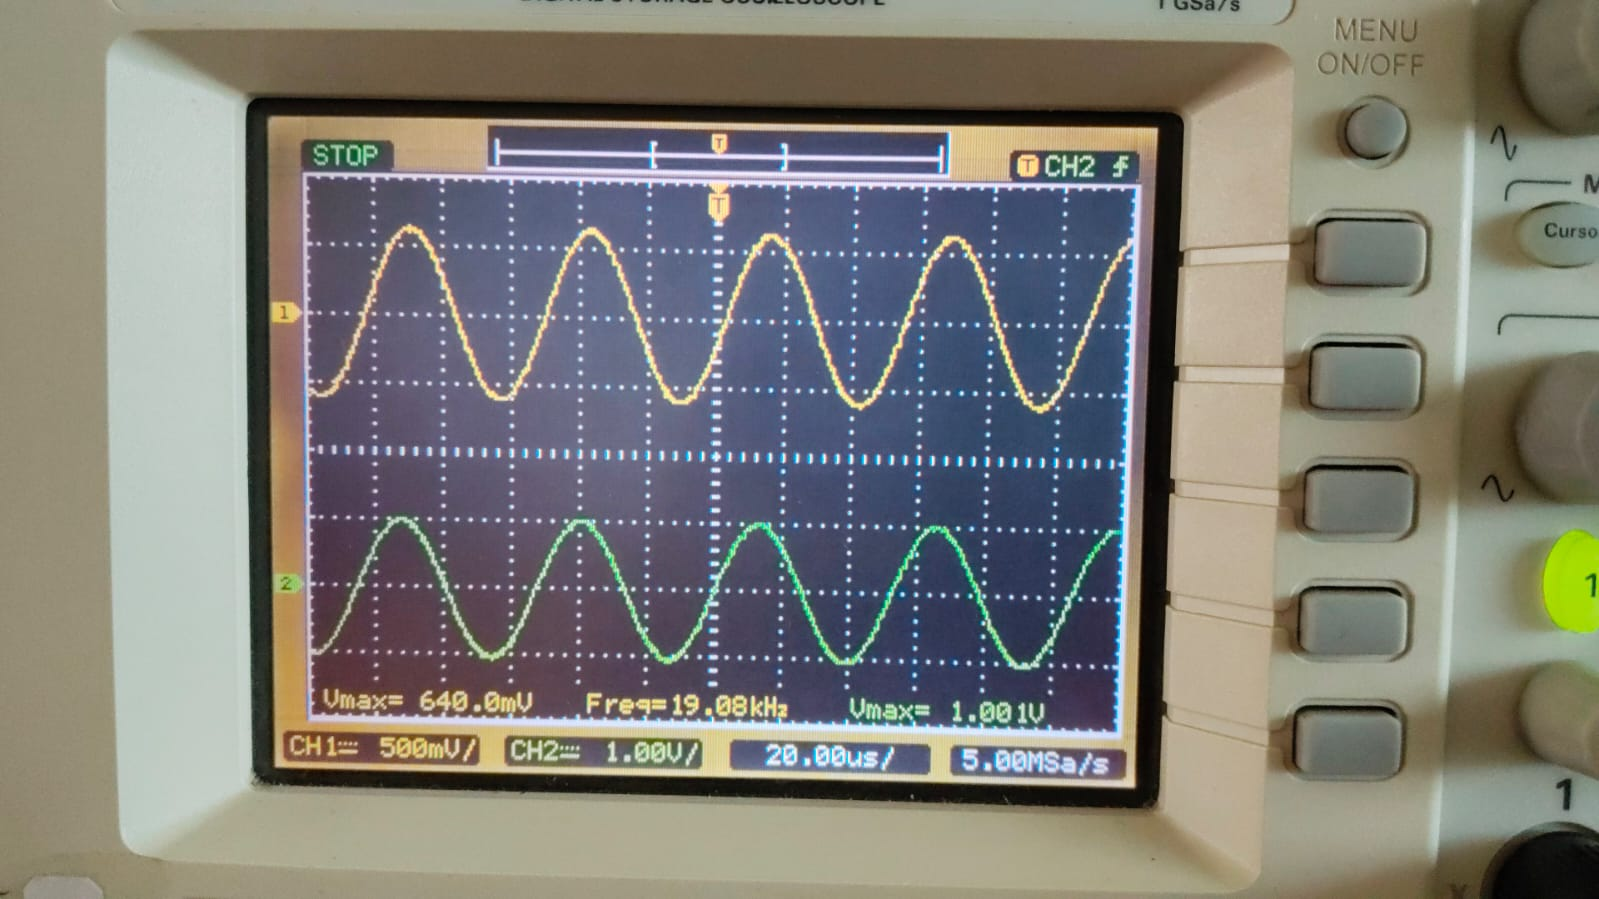
\includegraphics[width=0.45\textwidth]{figs/lpf_cutoff.jpeg}
    }
    \hfill
    \subfigure[]{
        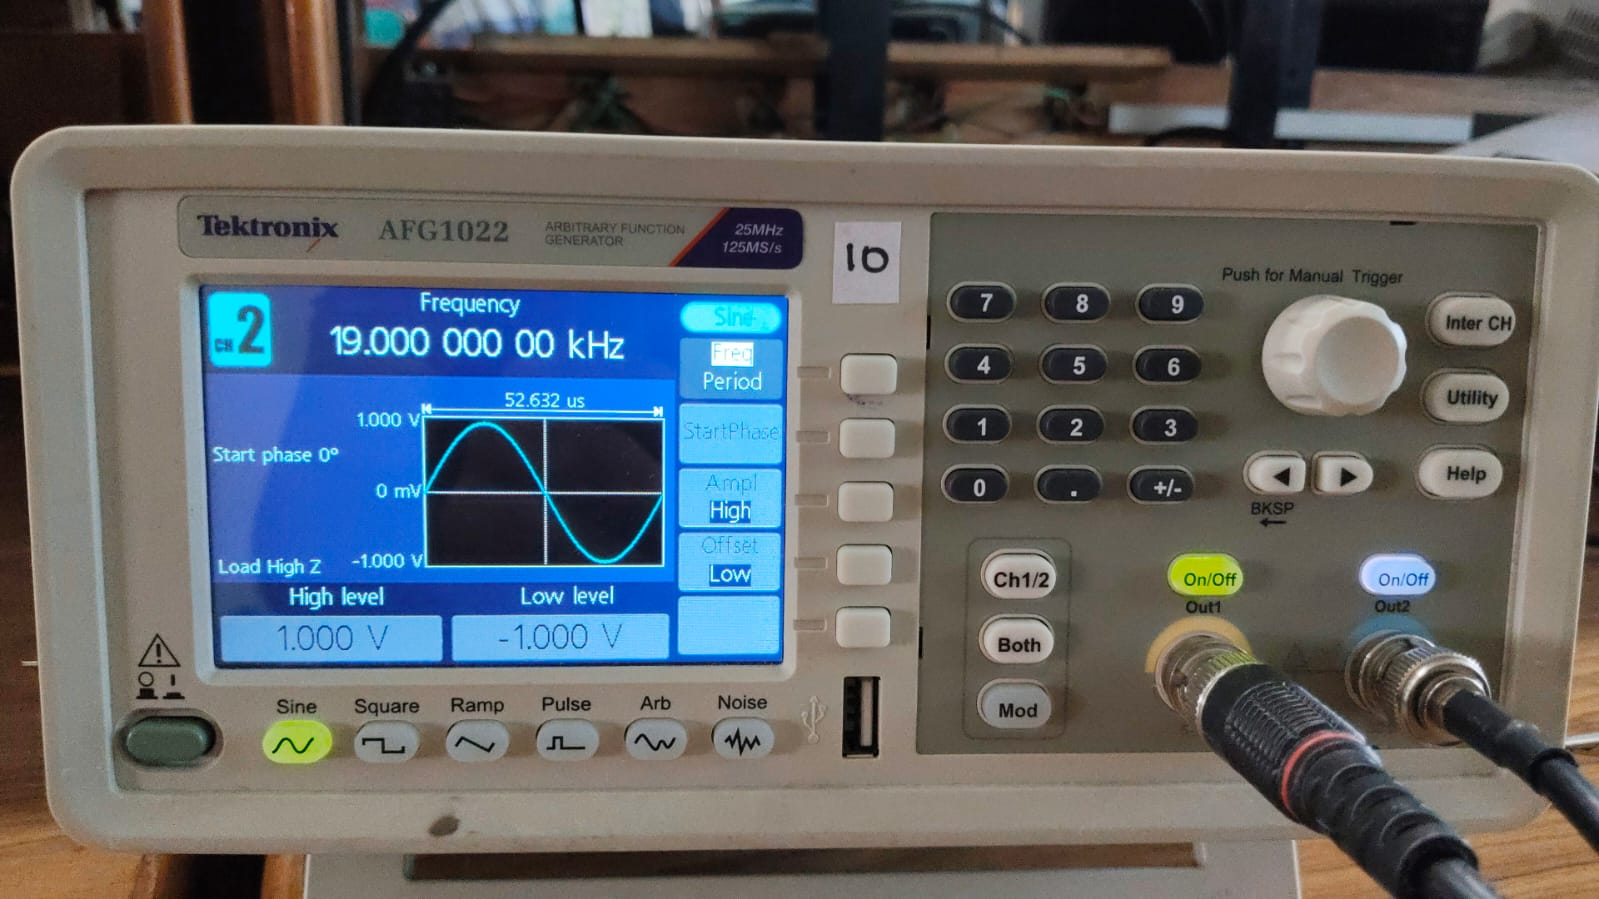
\includegraphics[width=0.45\textwidth]{figs/lpf_input_cutoff.jpeg}
    }
\end{figure}
\begin{figure}[H]
    \centering
    \subfigure[]{
        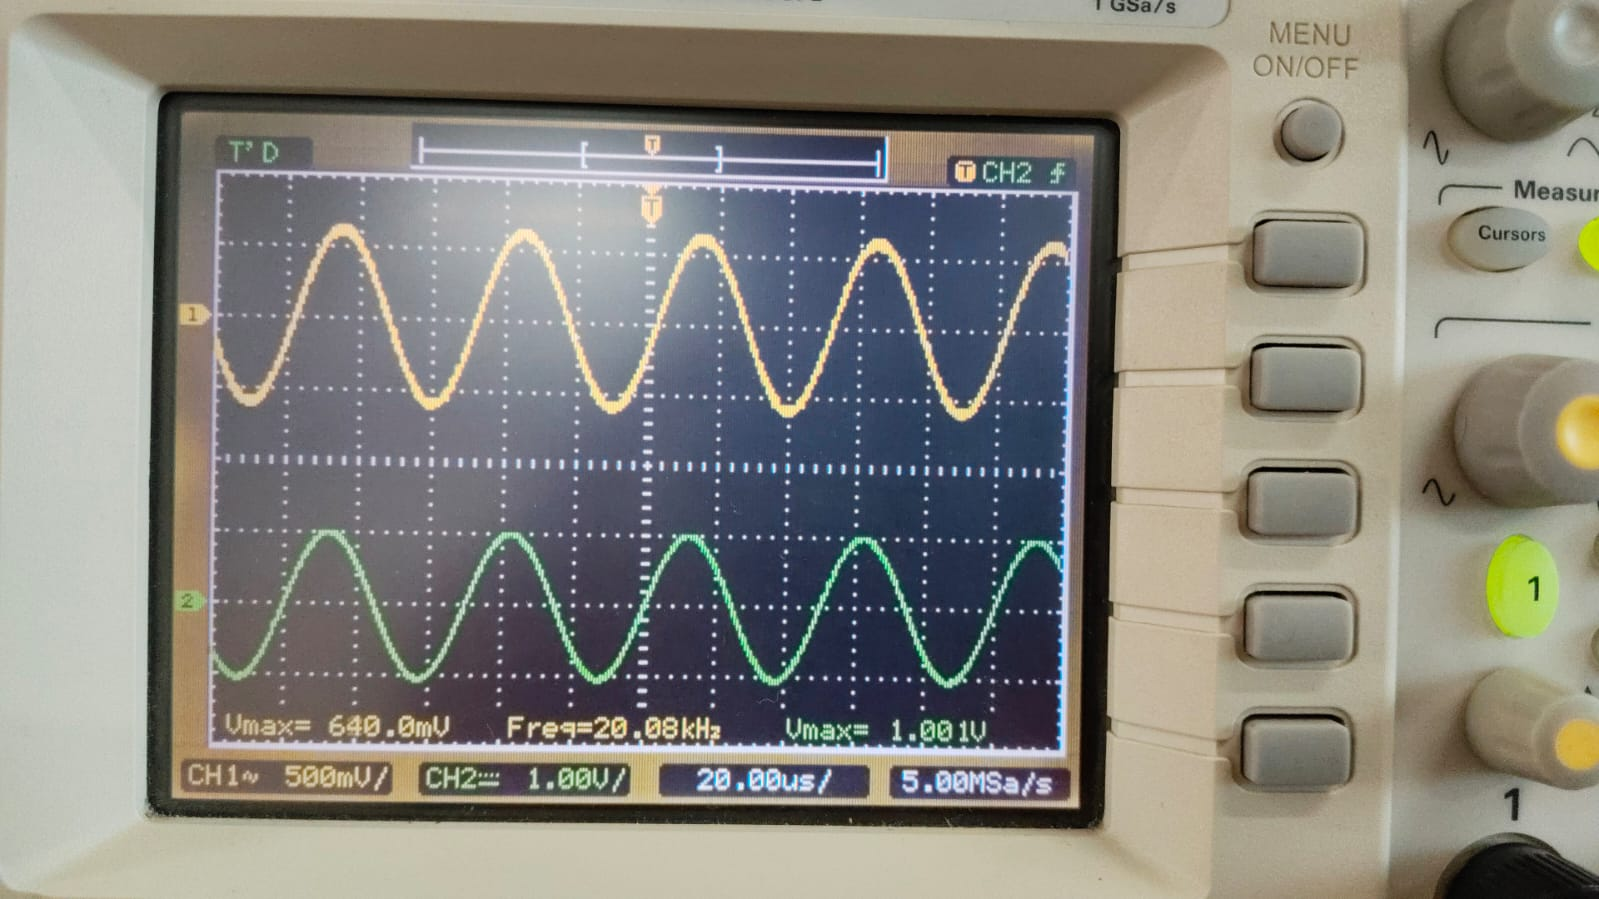
\includegraphics[width=0.45\textwidth]{figs/lpf_more_cutoff_1.jpeg}
    }
    \hfill
    \subfigure[]{
        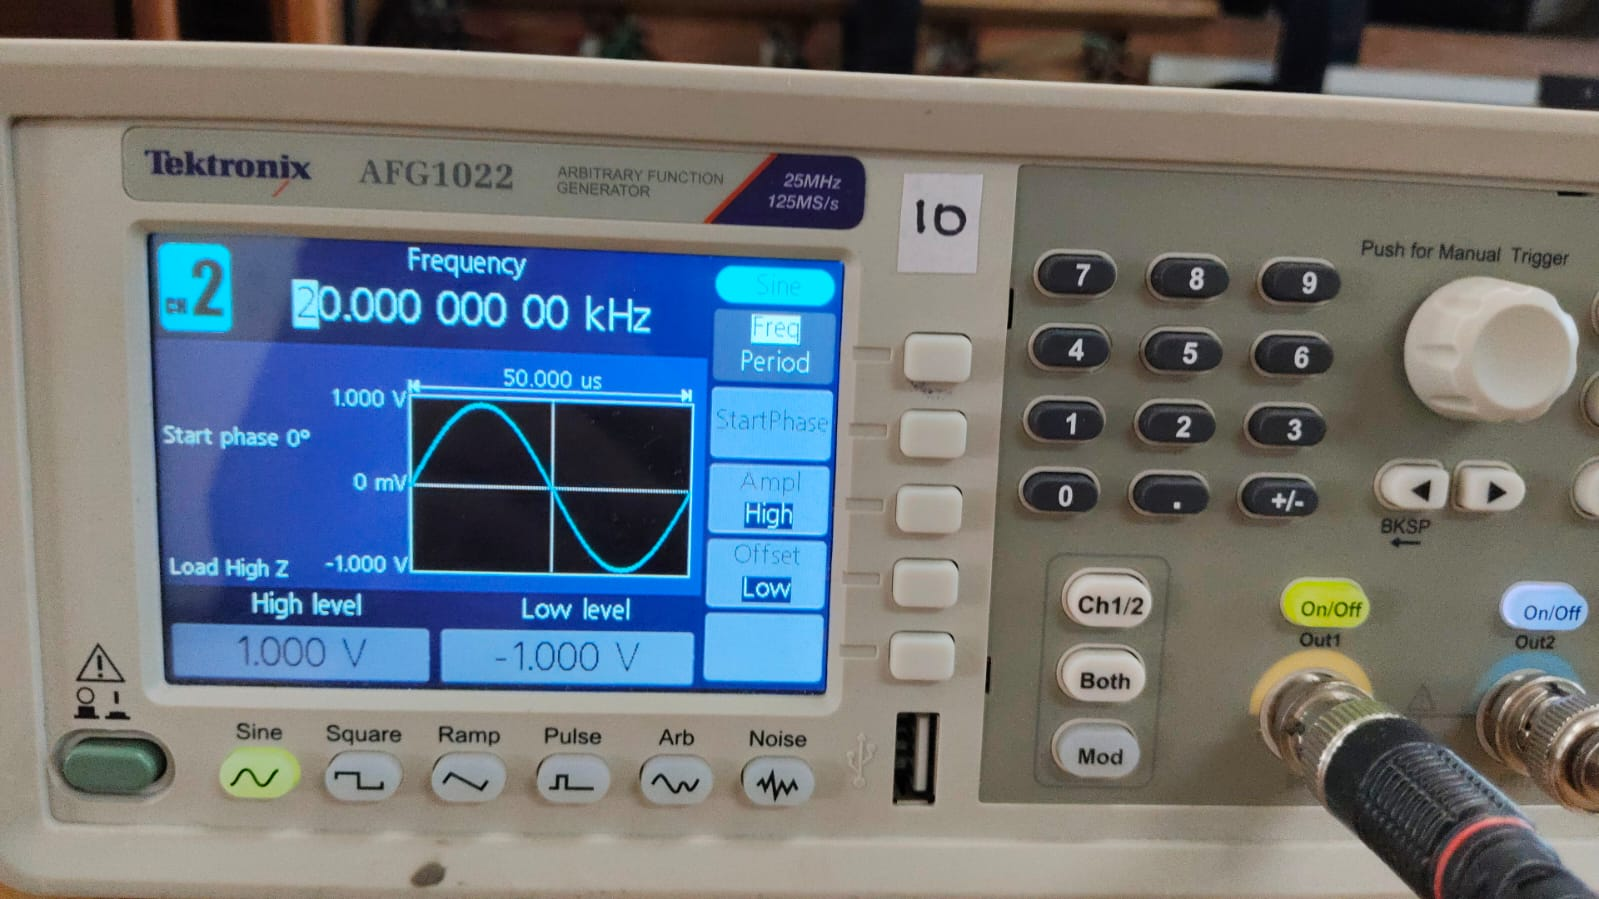
\includegraphics[width=0.45\textwidth]{figs/lpf_input_more_cutoff_1.jpeg}
    }
\end{figure}
\begin{figure}[H]
    \centering
    \subfigure[]{
        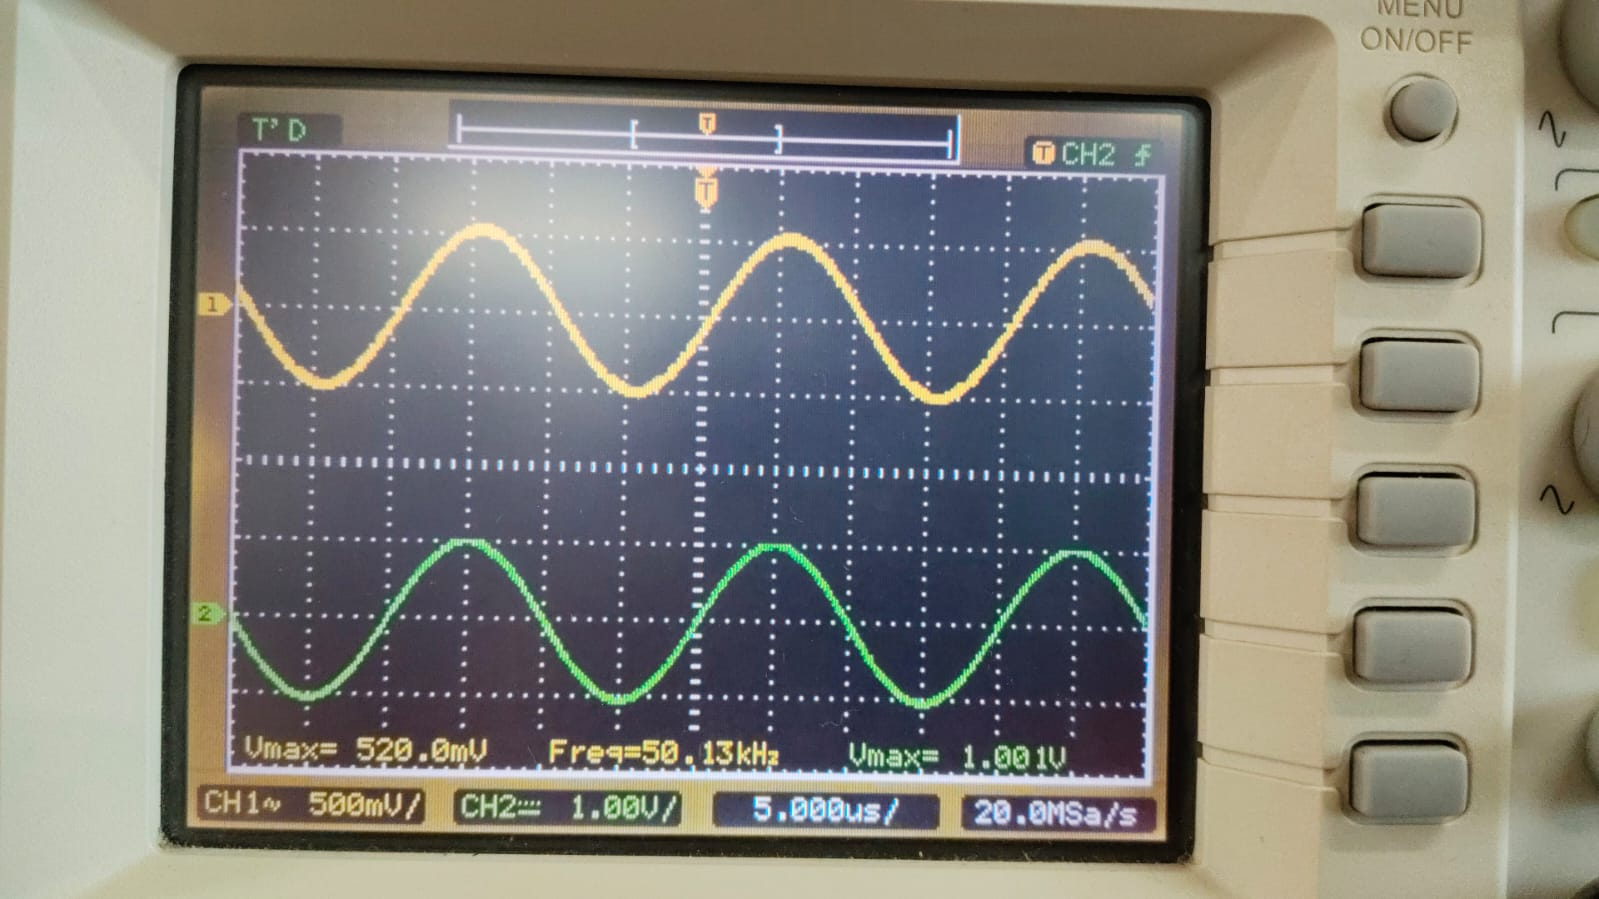
\includegraphics[width=0.45\textwidth]{figs/lpf_more_cutoff_2.jpeg}
    }
    \hfill
    \subfigure[]{
        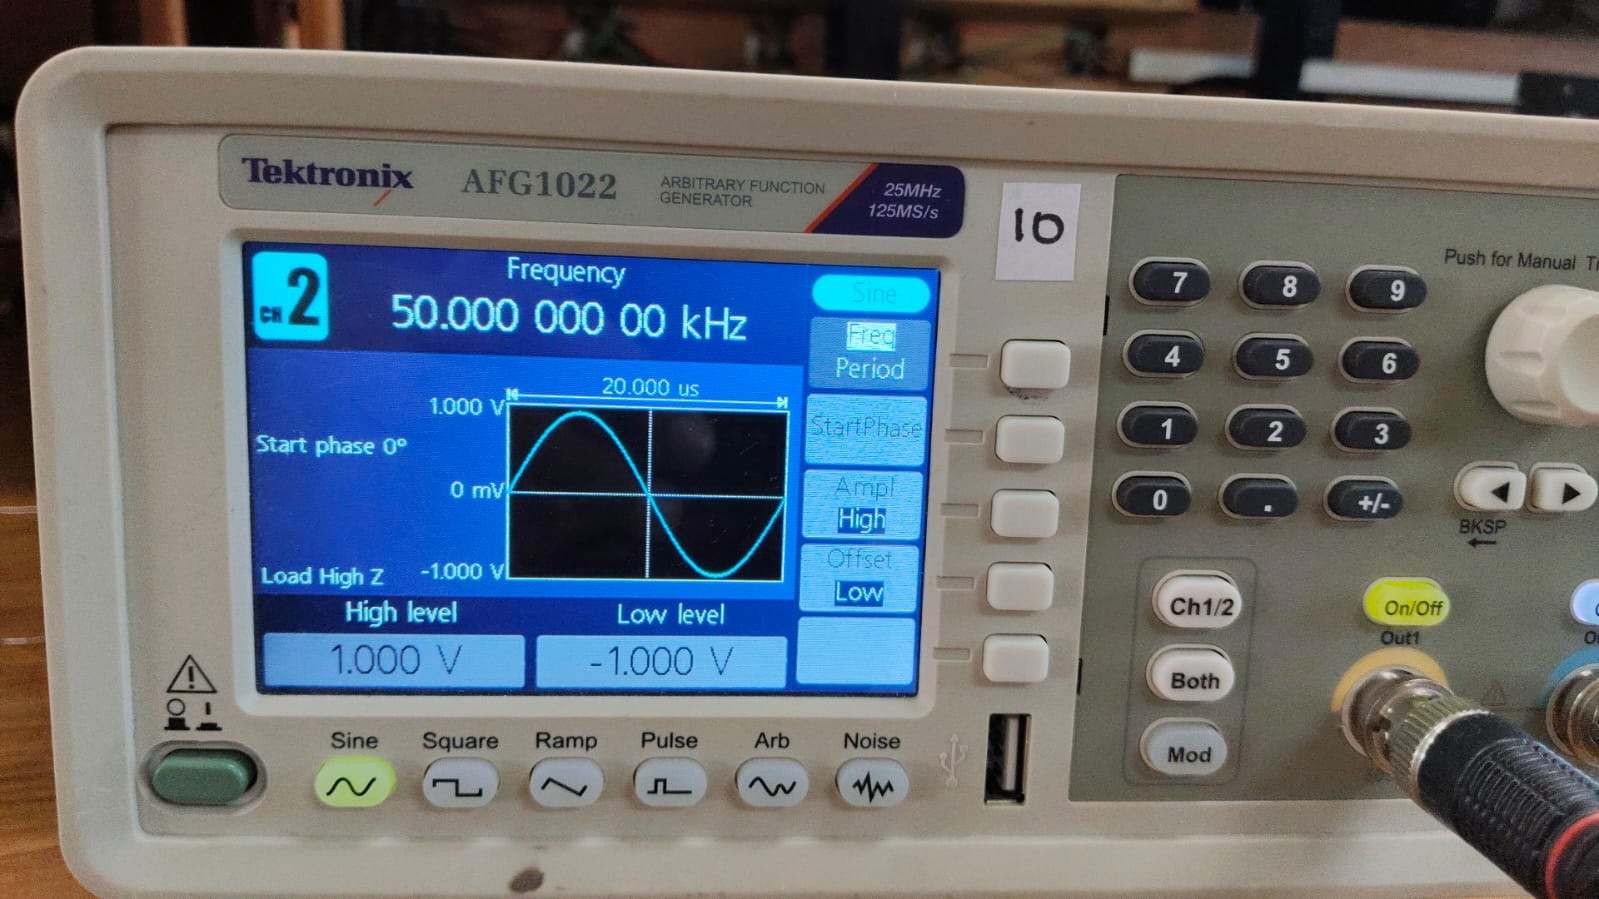
\includegraphics[width=0.45\textwidth]{figs/lpf_input_more_cutoff_2.jpeg}
    }
\end{figure}
\begin{figure}[H]
    \centering
    \subfigure[]{
        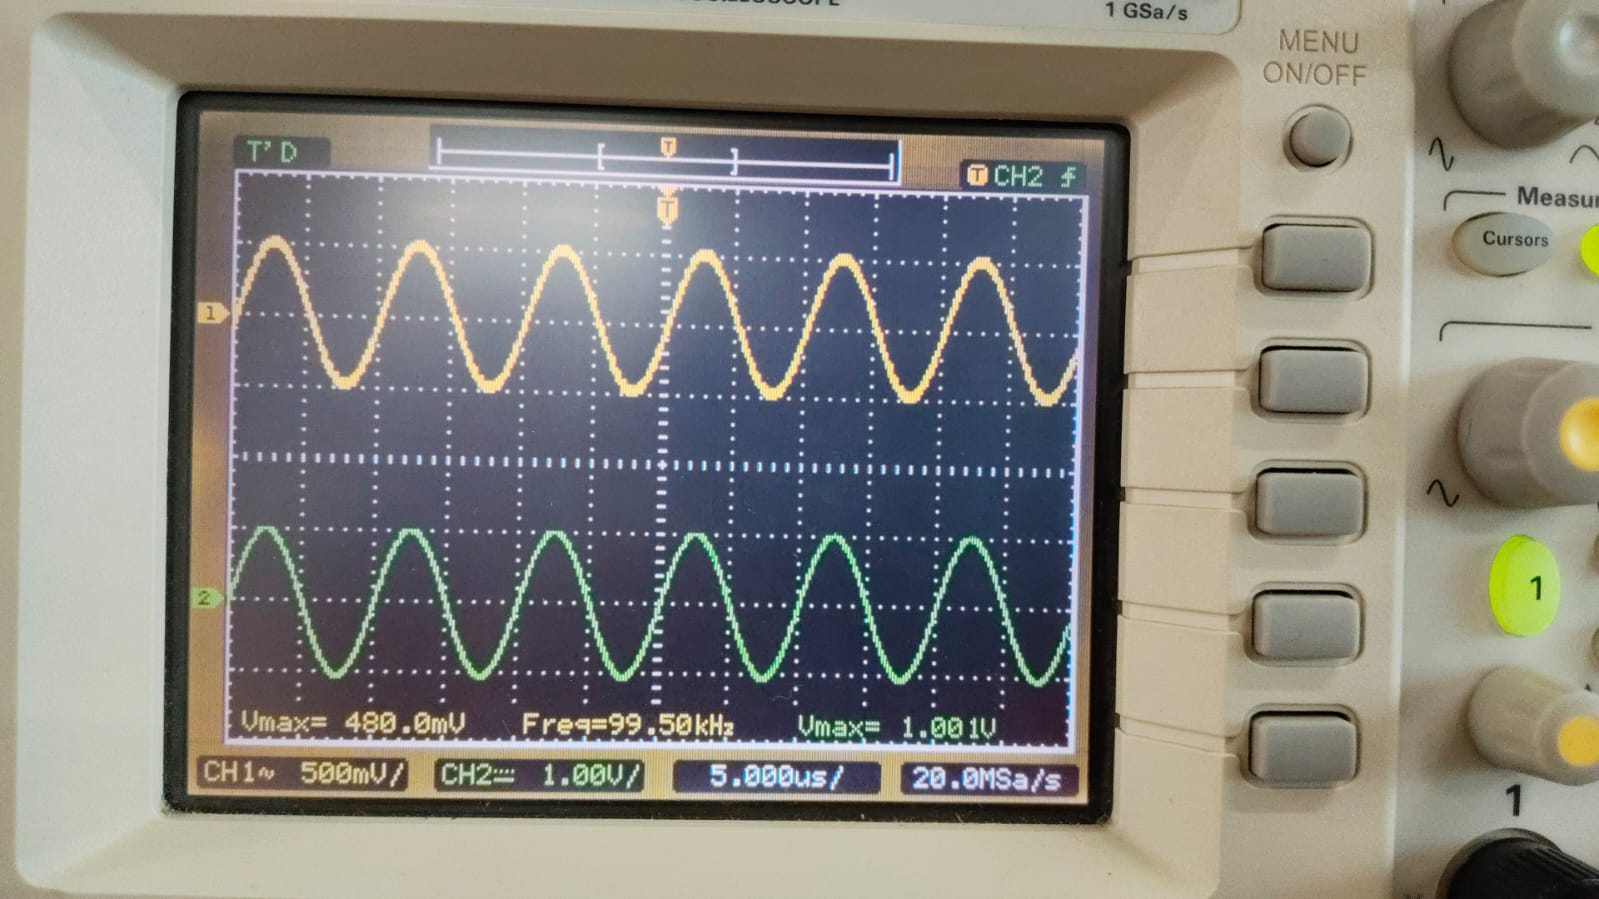
\includegraphics[width=0.45\textwidth]{figs/lpf_more_cutoff_3.jpeg}
    }
    \hfill
    \subfigure[]{
        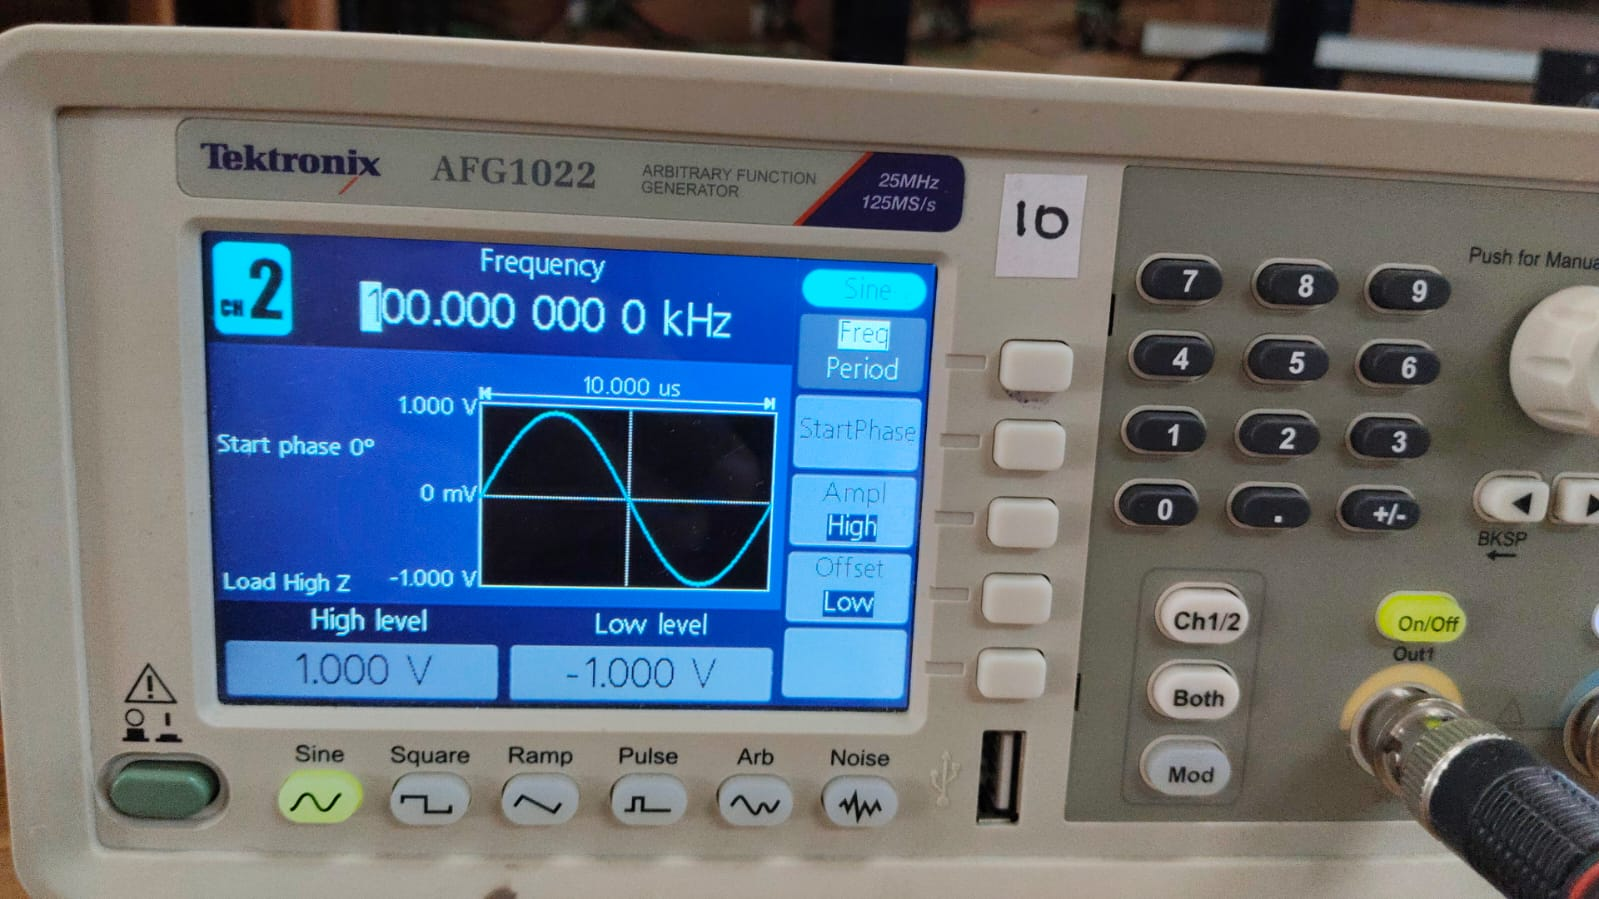
\includegraphics[width=0.45\textwidth]{figs/lpf_input_more_cutoff_3.jpeg}
    }
\end{figure}
\begin{figure}[H]
    \centering
    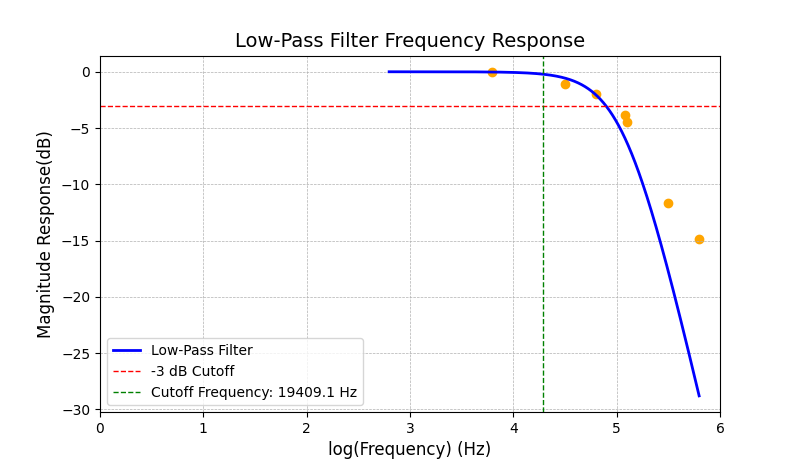
\includegraphics[width=\textwidth]{figs/low.png}
    \caption{Bode plot for LPF}
\end{figure}

\subsection{Bandpass Filter (BPF) Design}
A bandpass filter is formed by cascading the HPF and LPF, allowing signals within a specific frequency range to pass while attenuating frequencies outside this range. The important parameters are:
\begin{itemize}
    \item Bandwidth: $BW = f_{c2} - f_{c1}$
    \item Center Frequency: $f_0 = \sqrt{f_{c1} f_{c2}}$
\end{itemize}
Bandpass filters are widely used in wireless communication, biomedical signal processing, and audio applications to extract relevant signals within a desired frequency range.\\
\textbf{The values of Resistors in LPF part are:} 15ohm, 15ohm\\
\textbf{The values of Resistors in HPF part are:} 150ohm, 150ohm \\
\textbf{The values of Capacitors in LPF part are:} 1nF, 1nF \\
\textbf{The values of Capacitors in HPF part are:} 1nF, 1nF \\
\begin{figure}[H]
    \centering
    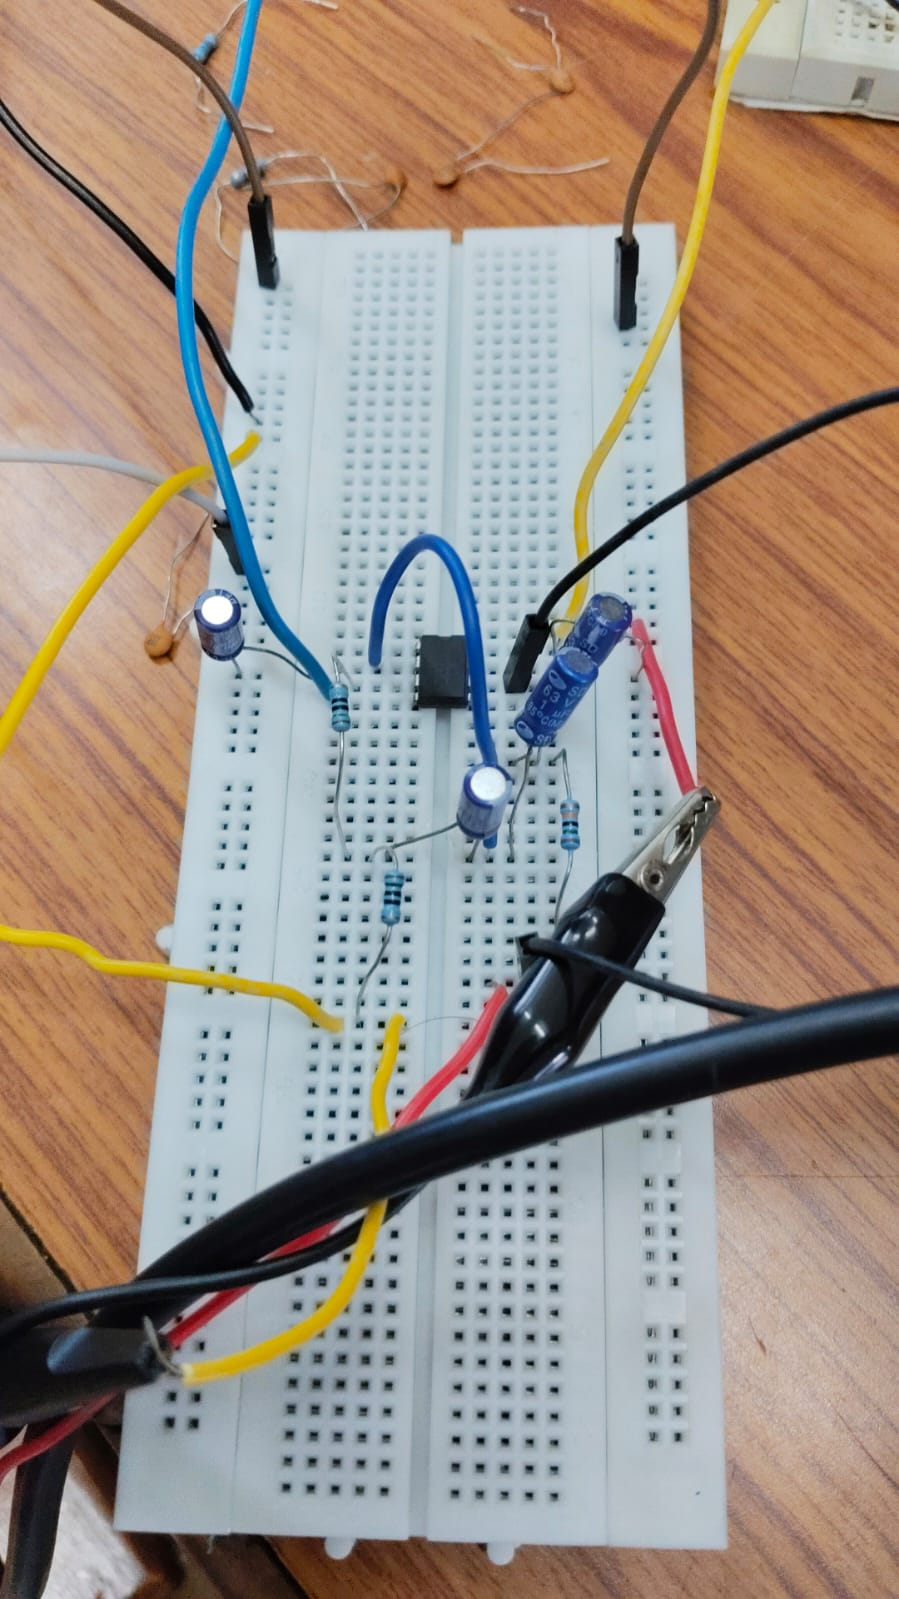
\includegraphics[width=0.4\textwidth]{figs/bpf_circuit.jpeg}
    \caption{Circuit for BPF}
\end{figure}
\begin{table}[H]
    \centering
    \renewcommand{\arraystretch}{1.3} % Adjust row height
    \begin{tabular}{|c|c|c|}
        \hline
        \textbf{S. No.} & \textbf{Input Frequency (Hz)} &\textbf{Output Voltage (V)} \\
        \hline
        1 & 5 & 2.801  \\
        2 & 10 & 3.681  \\
        3 & 31.6 & 4  \\
        4 & 100 & 4  \\
        5 & 250 & 3.761  \\
        6 & 500 & 3.121  \\
        7 & 1000 & 2.481  \\
        8 & 10000 & 1.681  \\
        9 & 100000 & 0.76  \\
        10 & 1000000 & 0.38  \\
        \hline
    \end{tabular}
    \caption{Observation Table for Frequency Response for BPF}
    \label{tab:observation}
\end{table}
\begin{figure}[H]
    \centering
    \subfigure[]{
        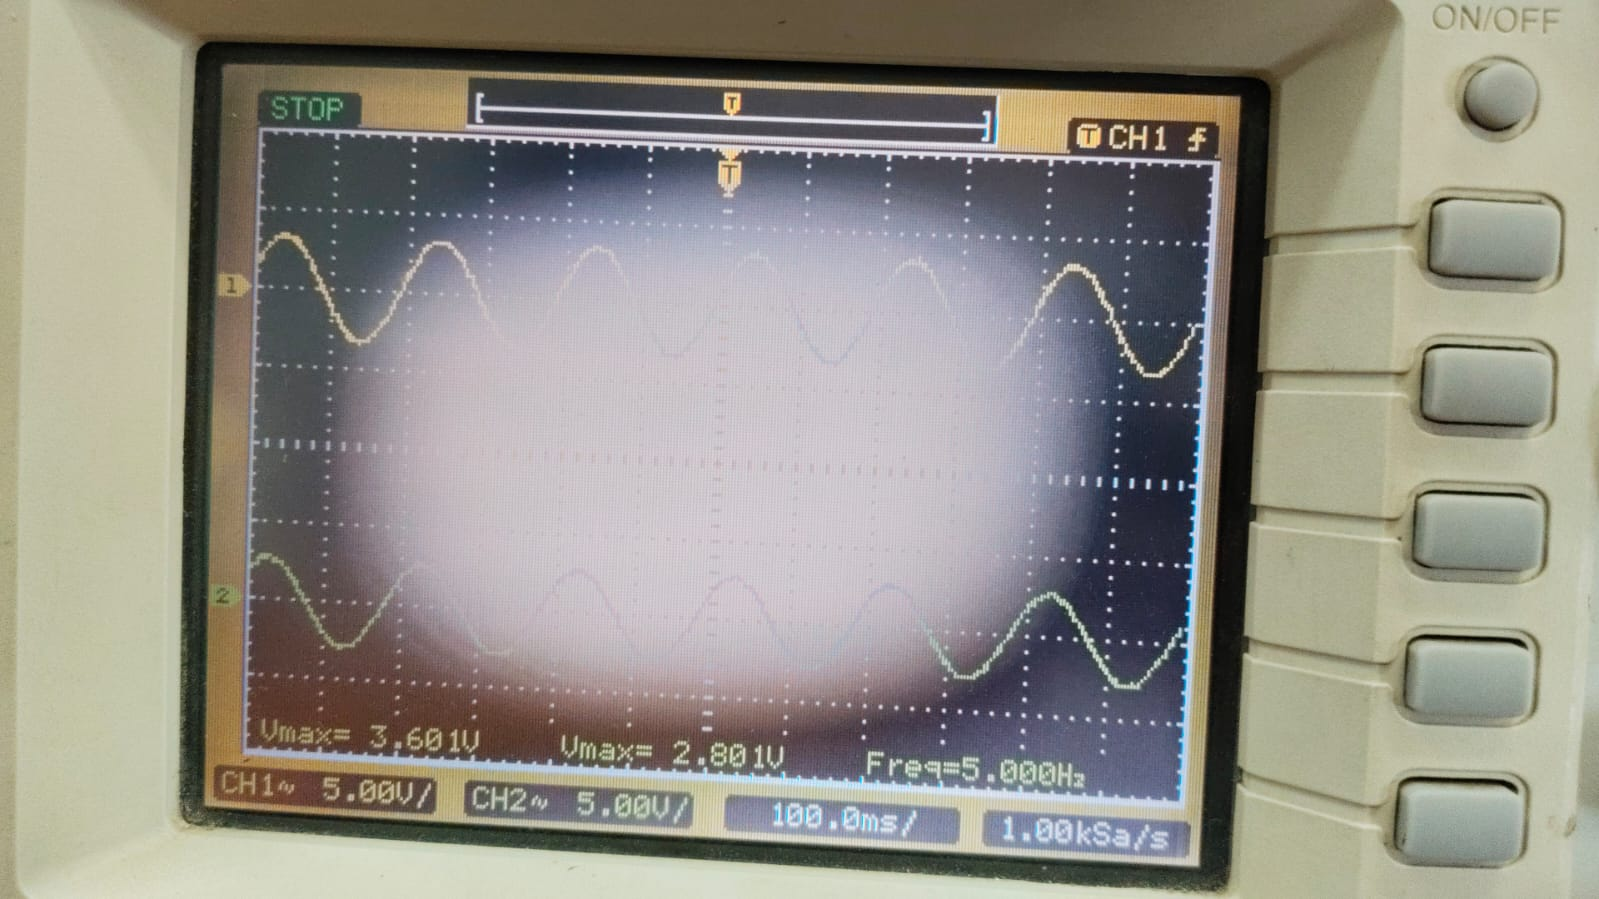
\includegraphics[width=0.45\textwidth]{figs/bpf_between_5.jpeg}
    }
    \hfill
    \subfigure[]{
        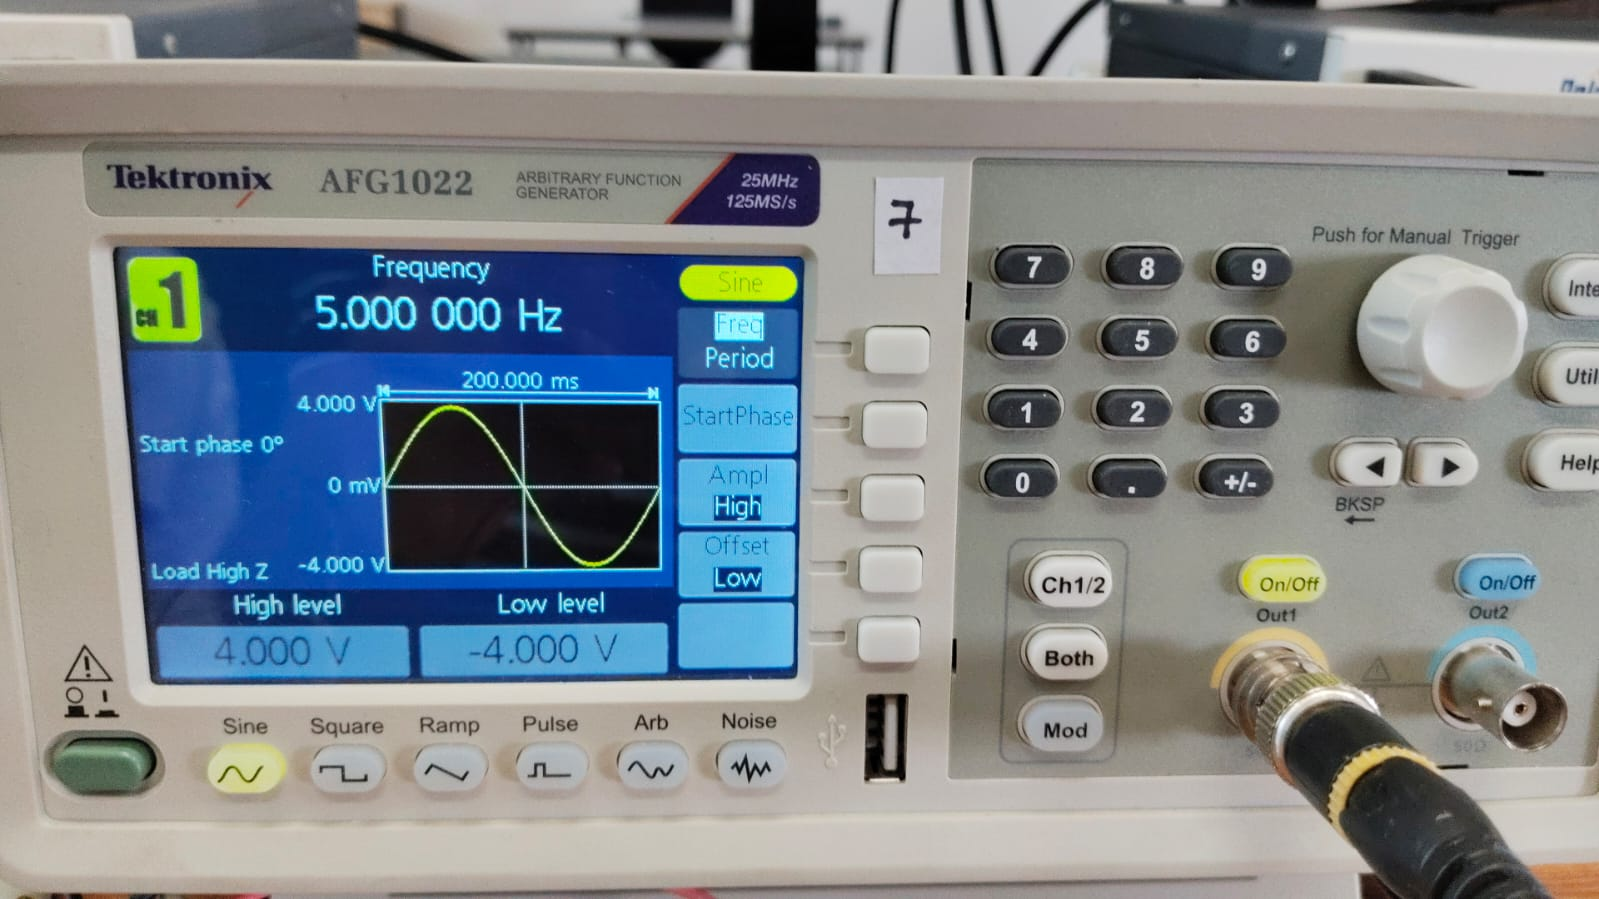
\includegraphics[width=0.45\textwidth]{figs/bpf_input_between_5.jpeg}
    }
\end{figure}
\begin{figure}[H]
    \centering
    \subfigure[]{
        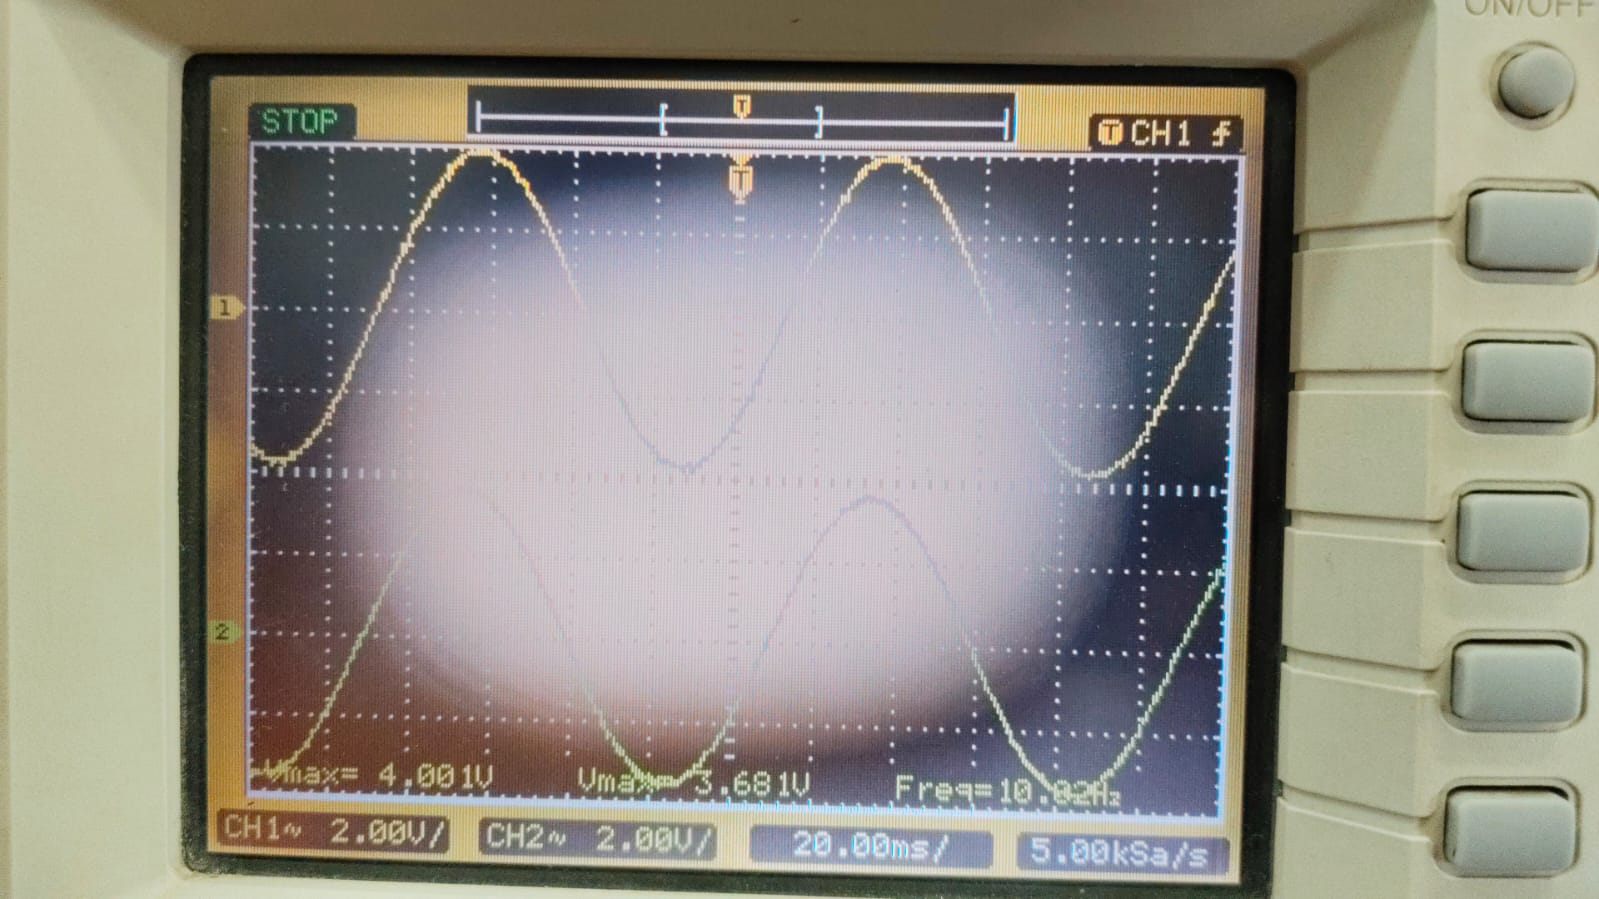
\includegraphics[width=0.45\textwidth]{figs/bpf_between_4.jpeg}
    }
    \hfill
    \subfigure[]{
        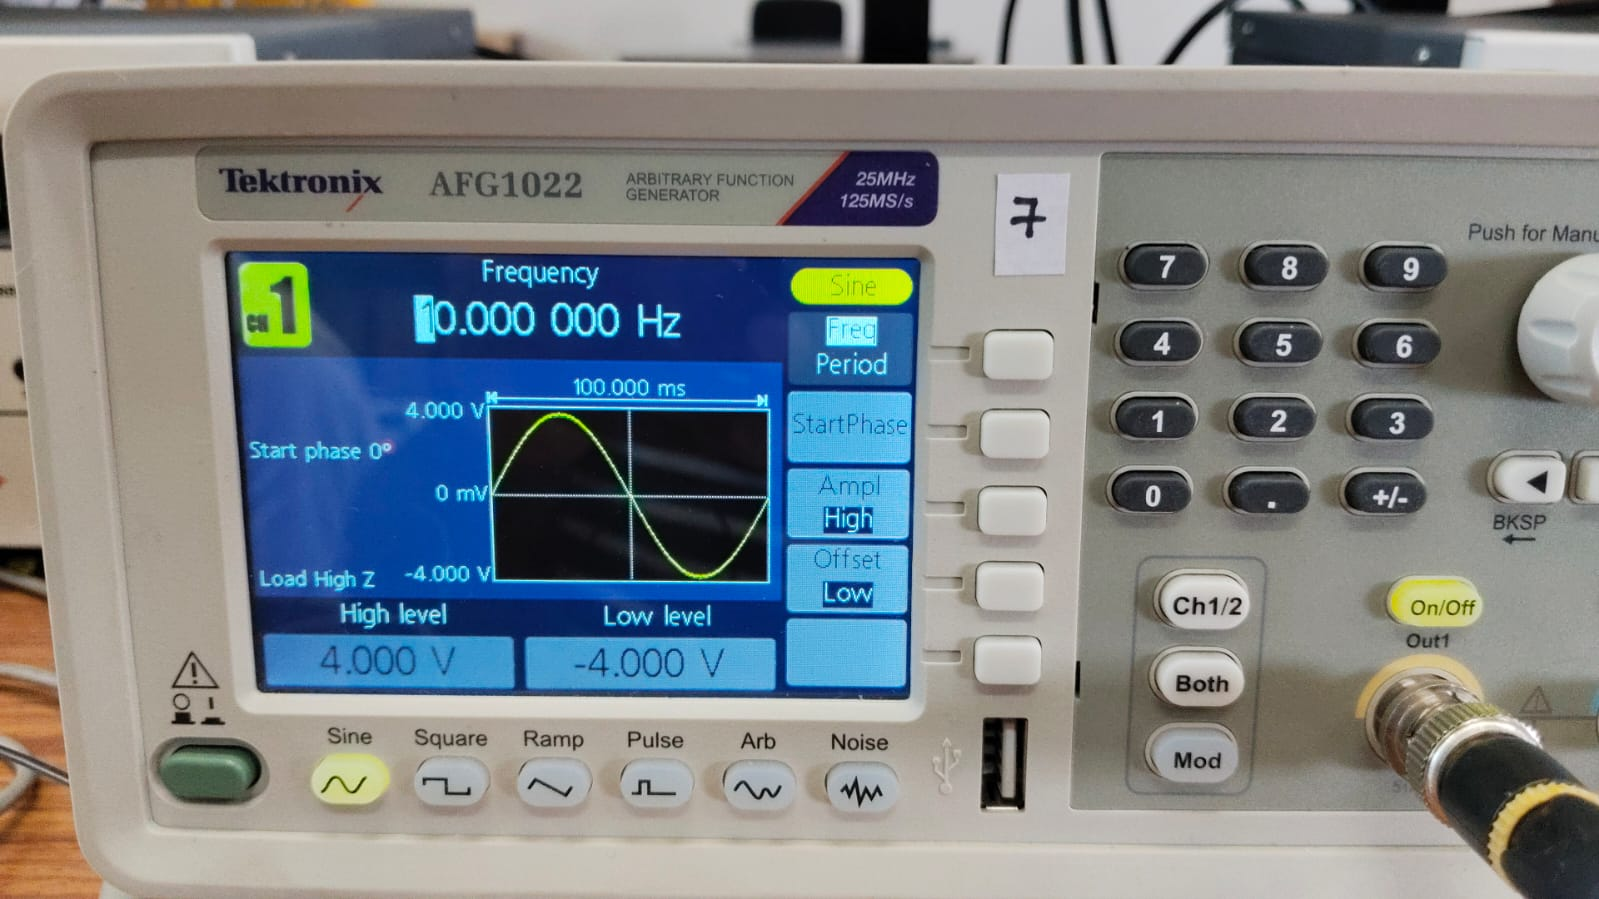
\includegraphics[width=0.45\textwidth]{figs/bpf_input_between_4.jpeg}
    }
\end{figure}
\begin{figure}[H]
    \centering
    \subfigure[]{
        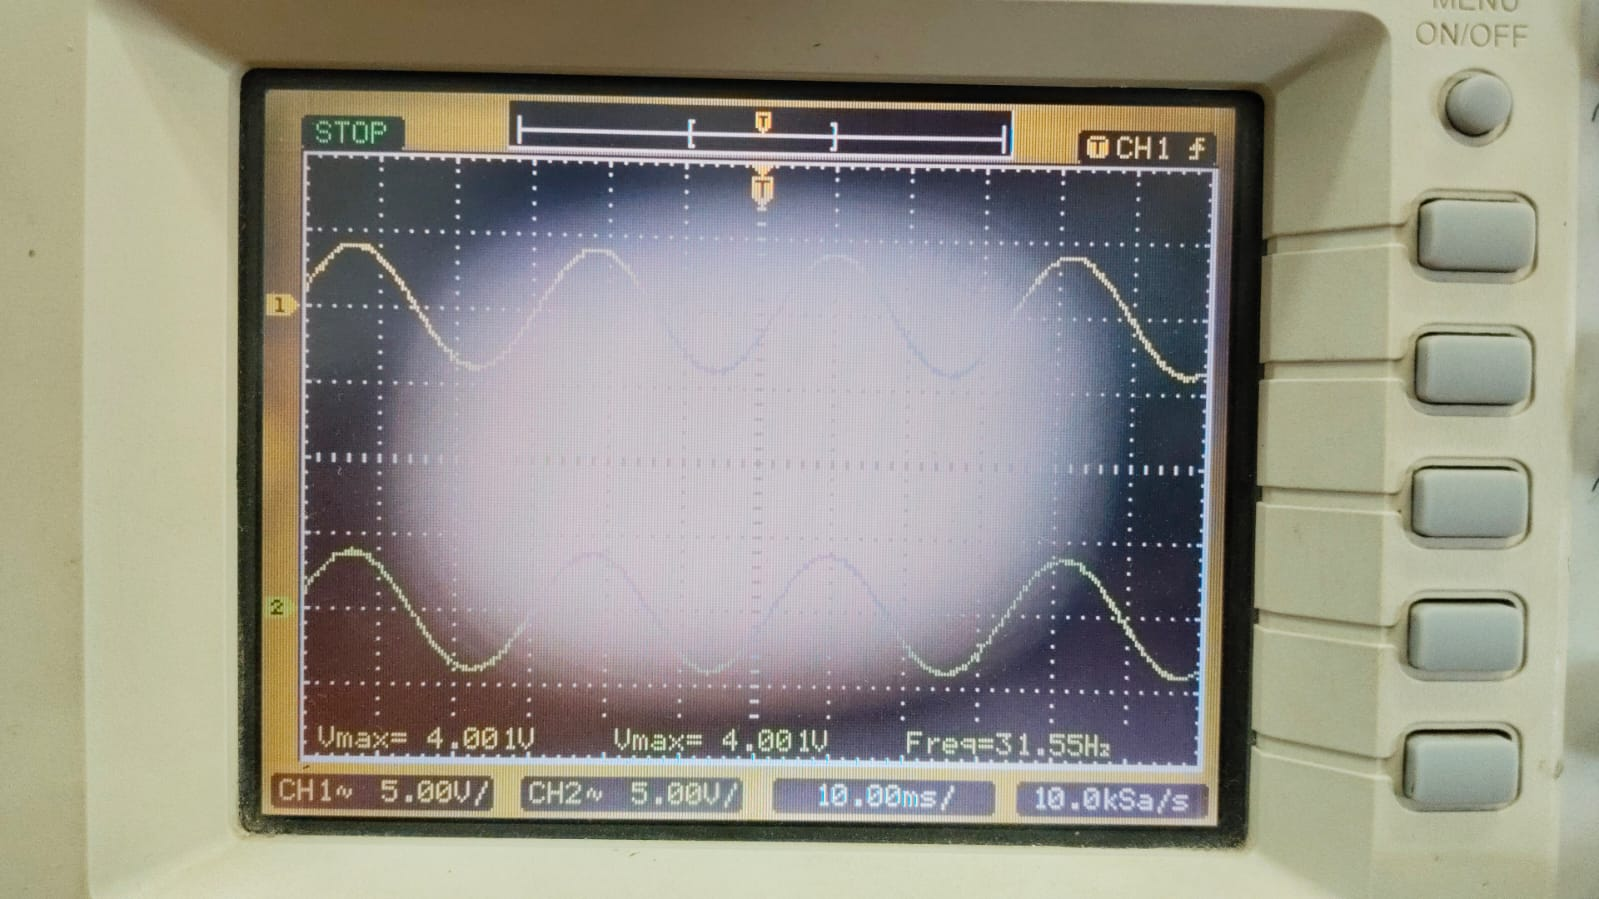
\includegraphics[width=0.45\textwidth]{figs/bpf_cutoff.jpeg}
    }
    \hfill
    \subfigure[]{
        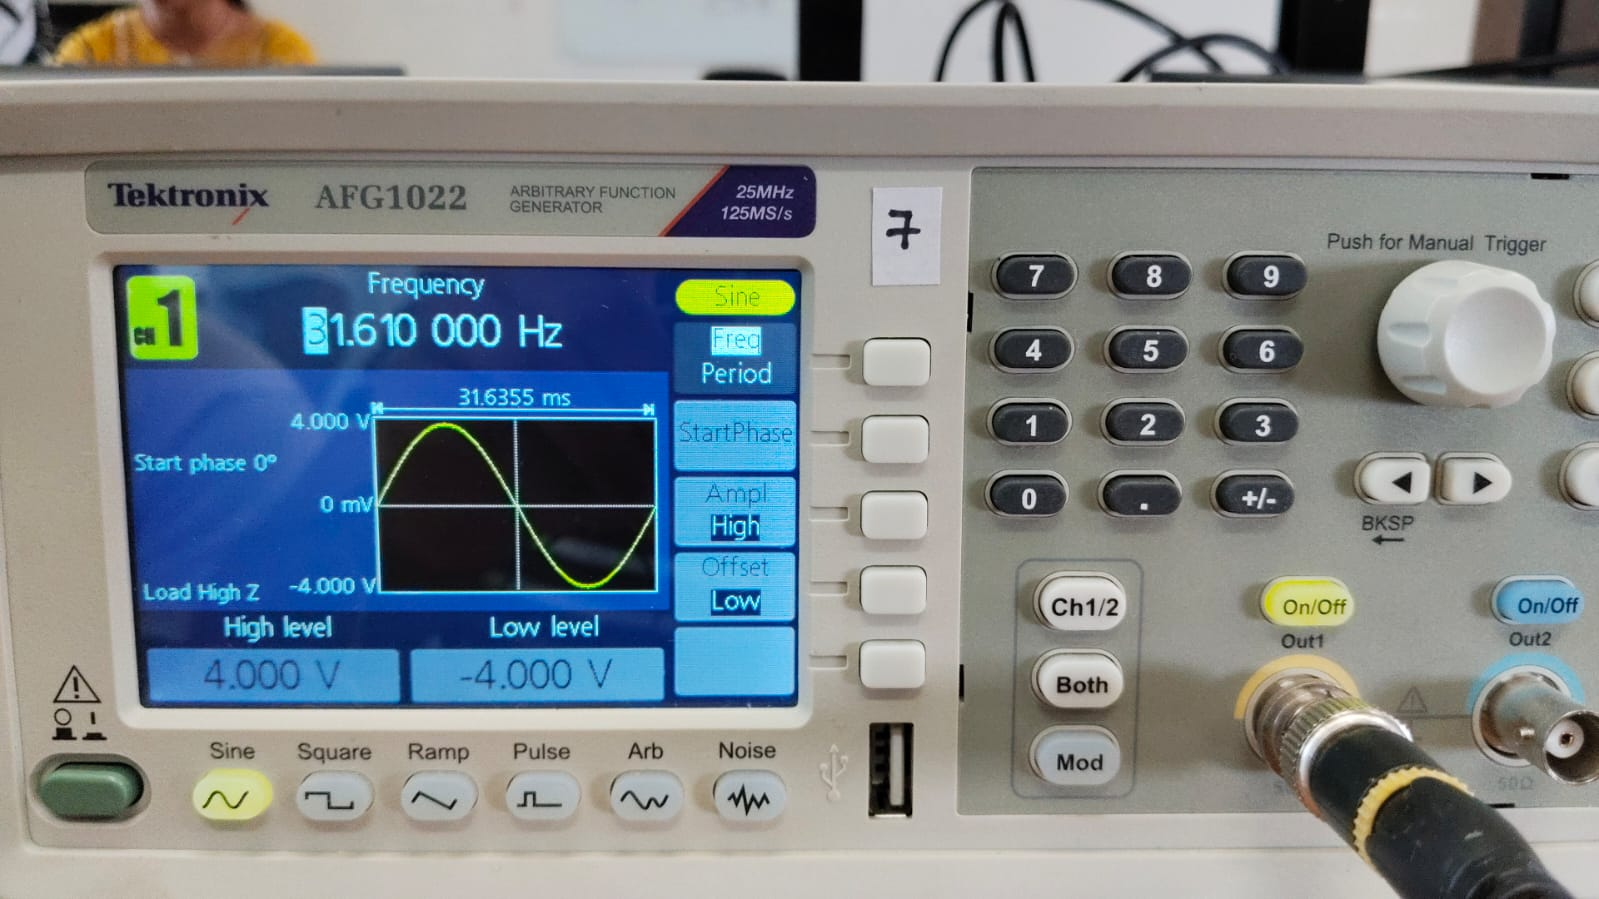
\includegraphics[width=0.45\textwidth]{figs/bpf_input_cutoff.jpeg}
    }
\end{figure}
\begin{figure}[H]
    \centering
    \subfigure[]{
        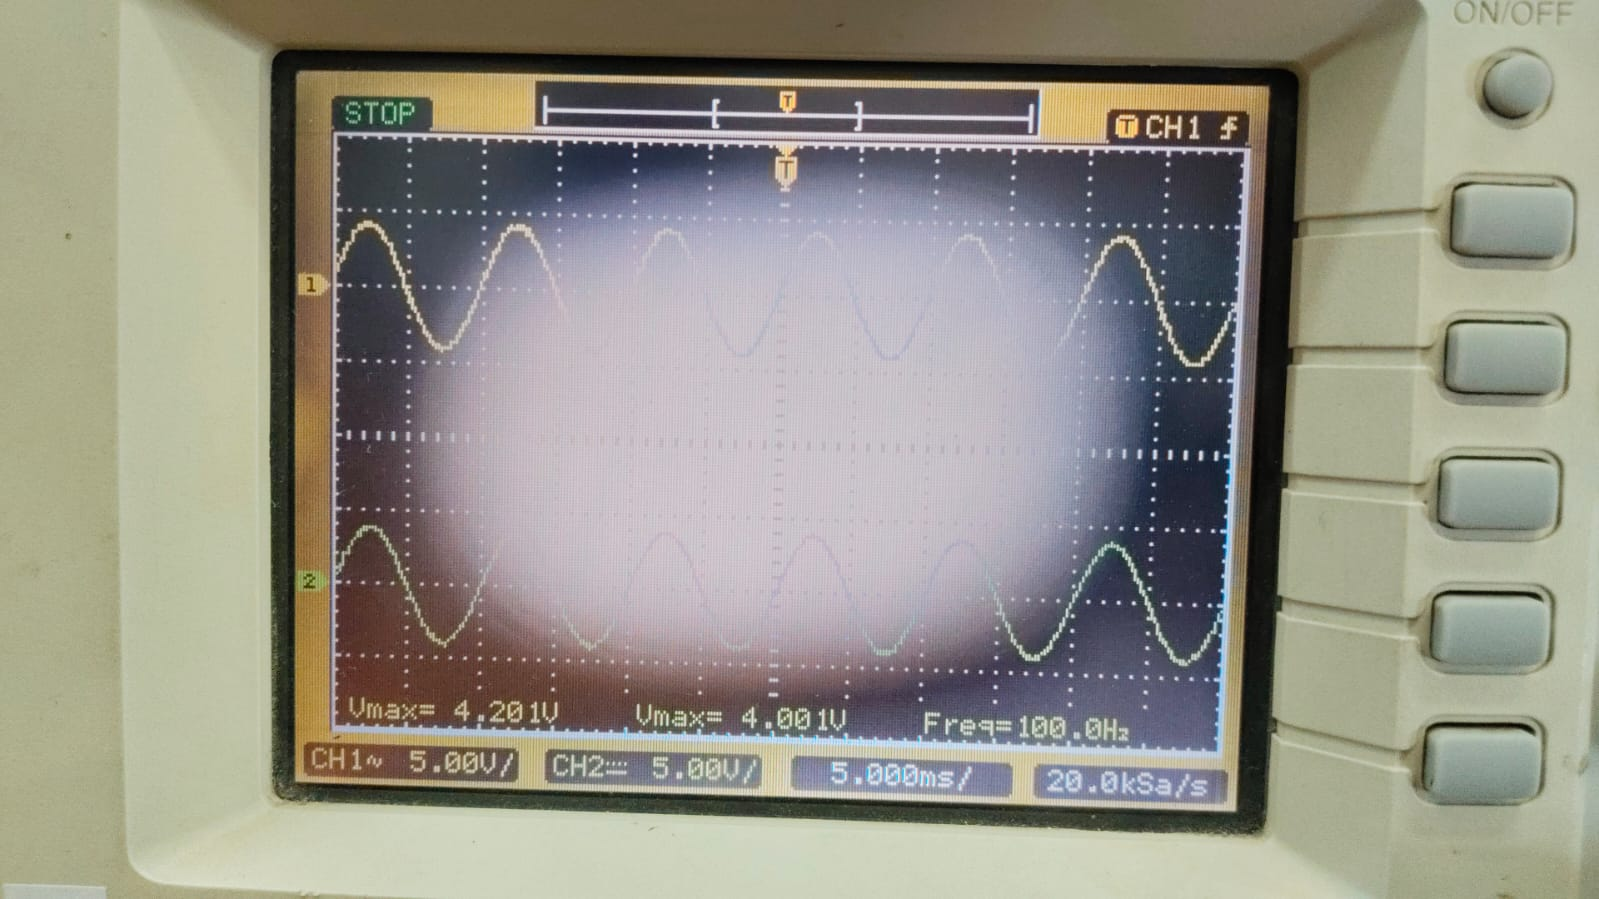
\includegraphics[width=0.45\textwidth]{figs/bpf_between_3.jpeg}
    }
    \hfill
    \subfigure[]{
        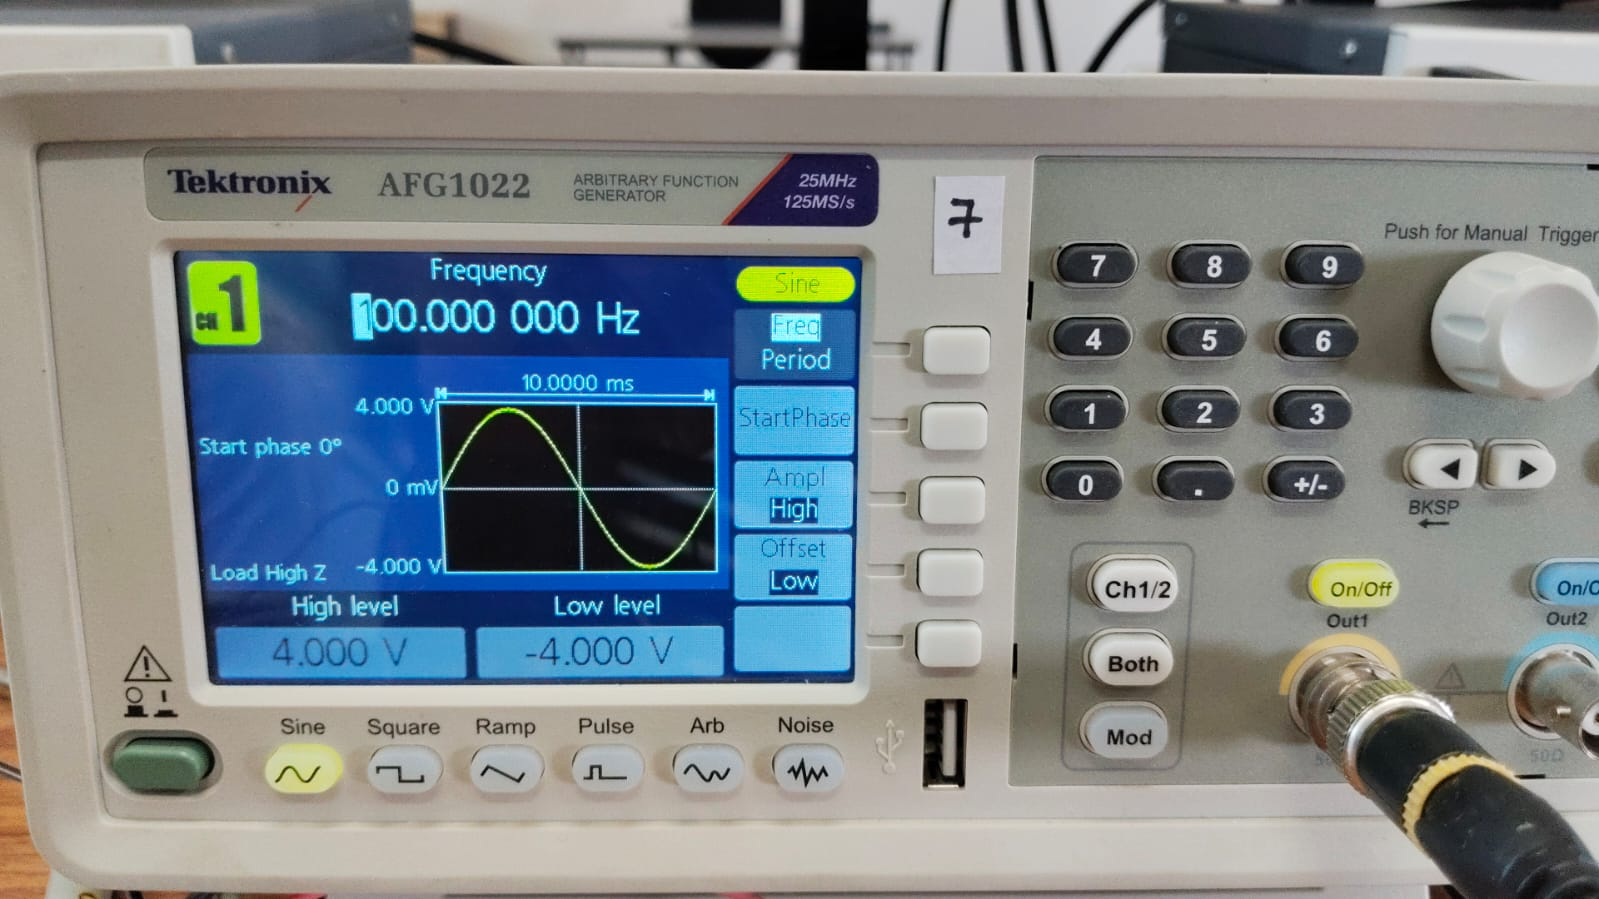
\includegraphics[width=0.45\textwidth]{figs/bpf_input_between_3.jpeg}
    }
\end{figure}
\begin{figure}[H]
    \centering
    \subfigure[]{
        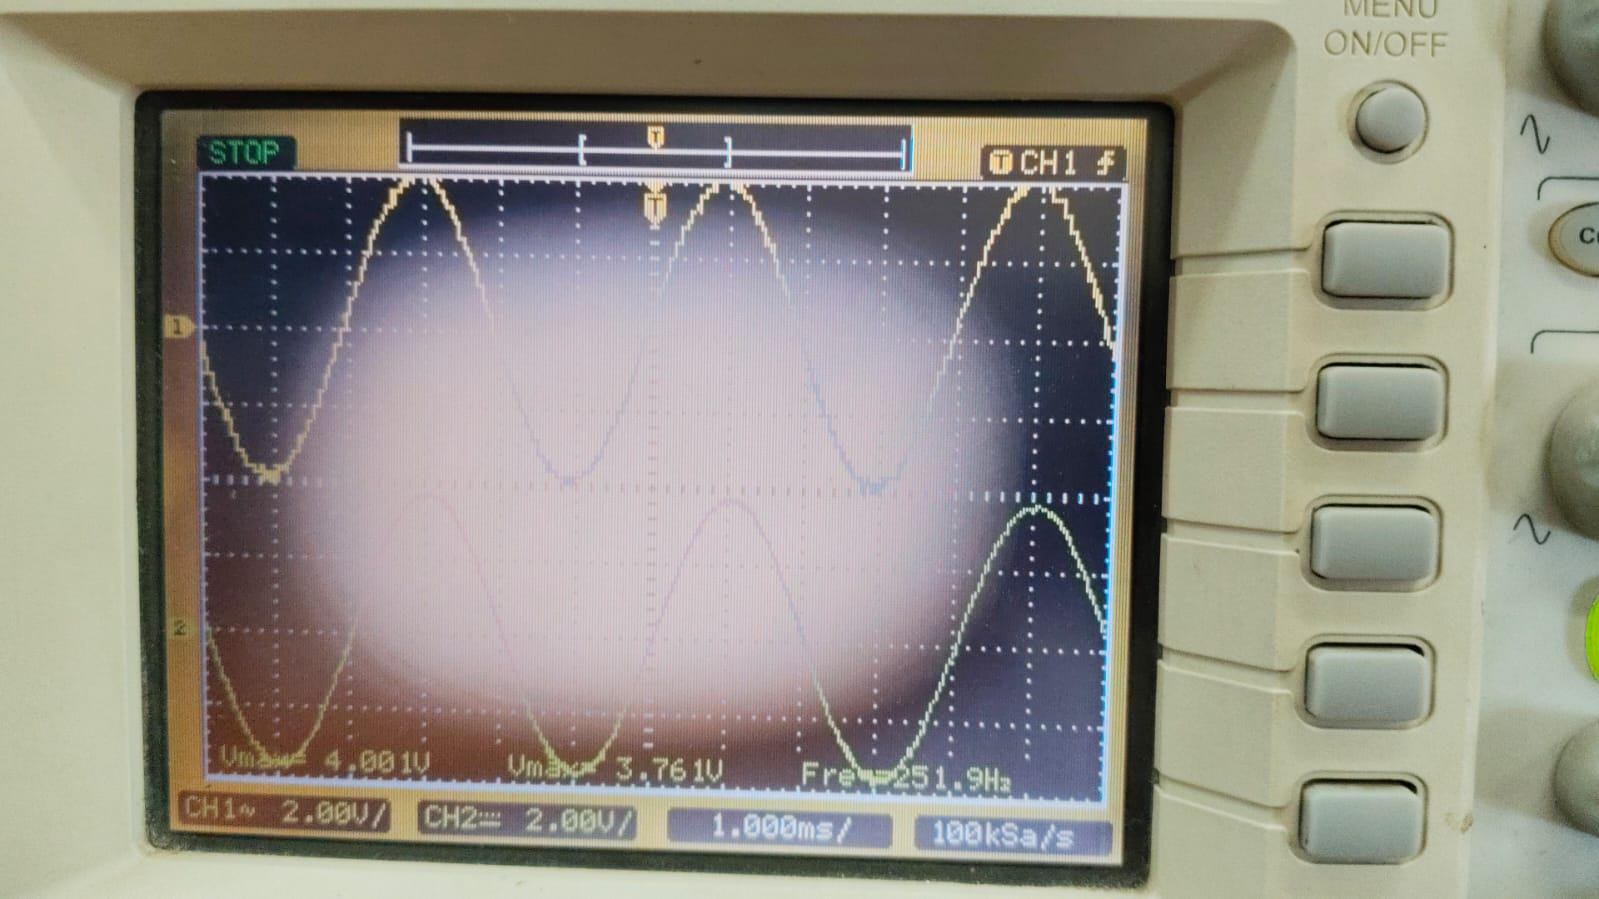
\includegraphics[width=0.45\textwidth]{figs/bpf_between_2.jpeg}
    }
    \hfill
    \subfigure[]{
        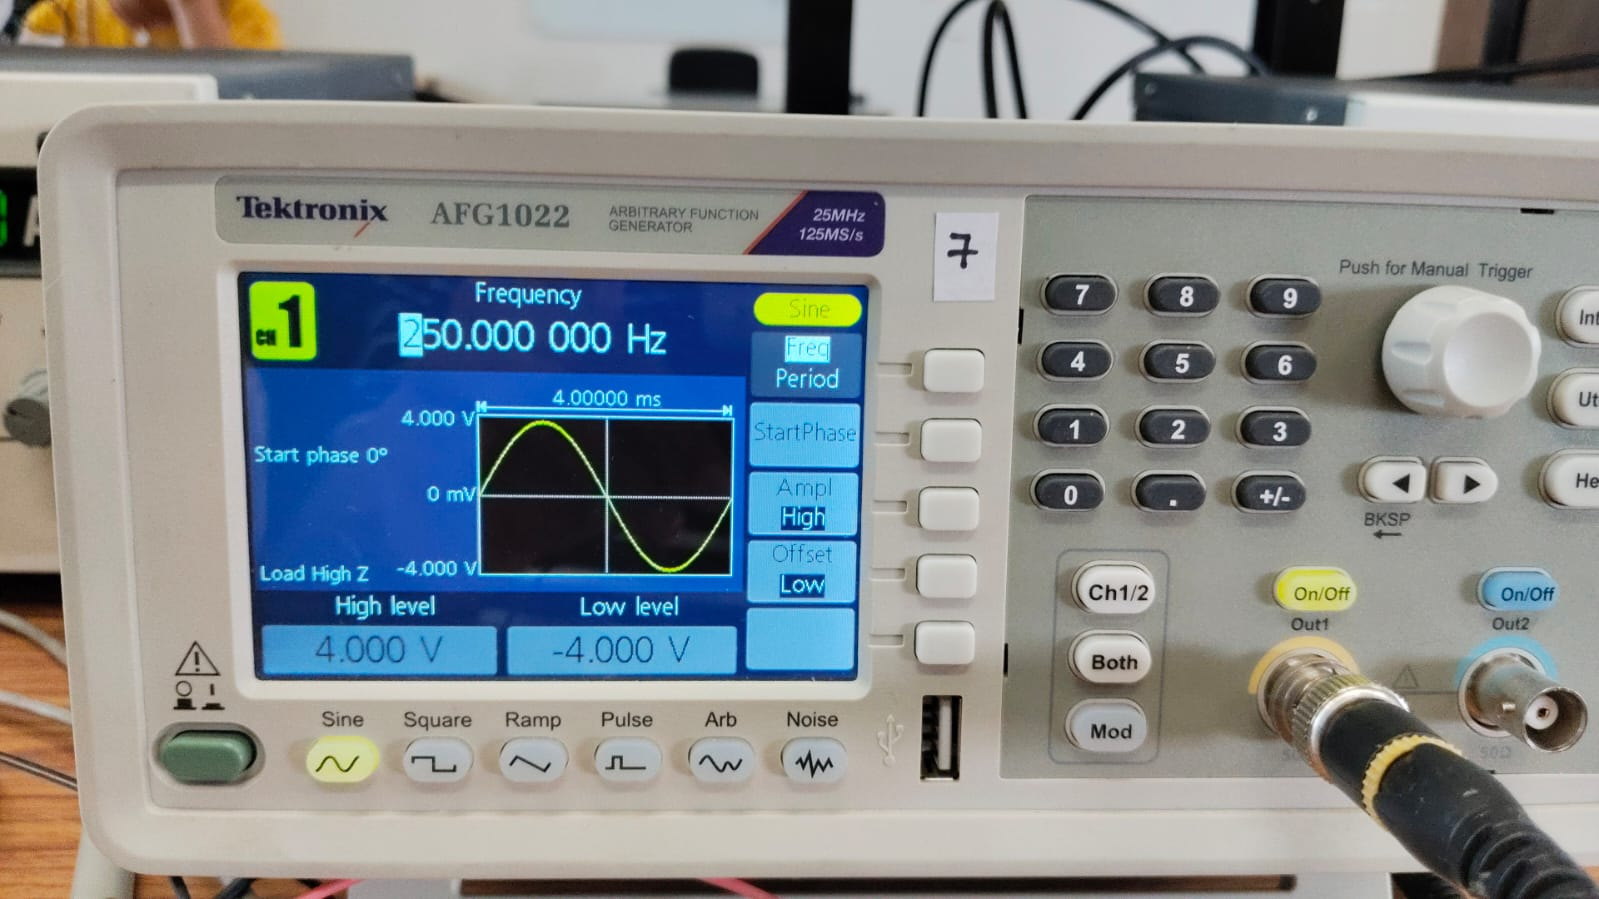
\includegraphics[width=0.45\textwidth]{figs/bpf_input_between_2.jpeg}
    }
\end{figure}
\begin{figure}[H]
    \centering
    \subfigure[]{
        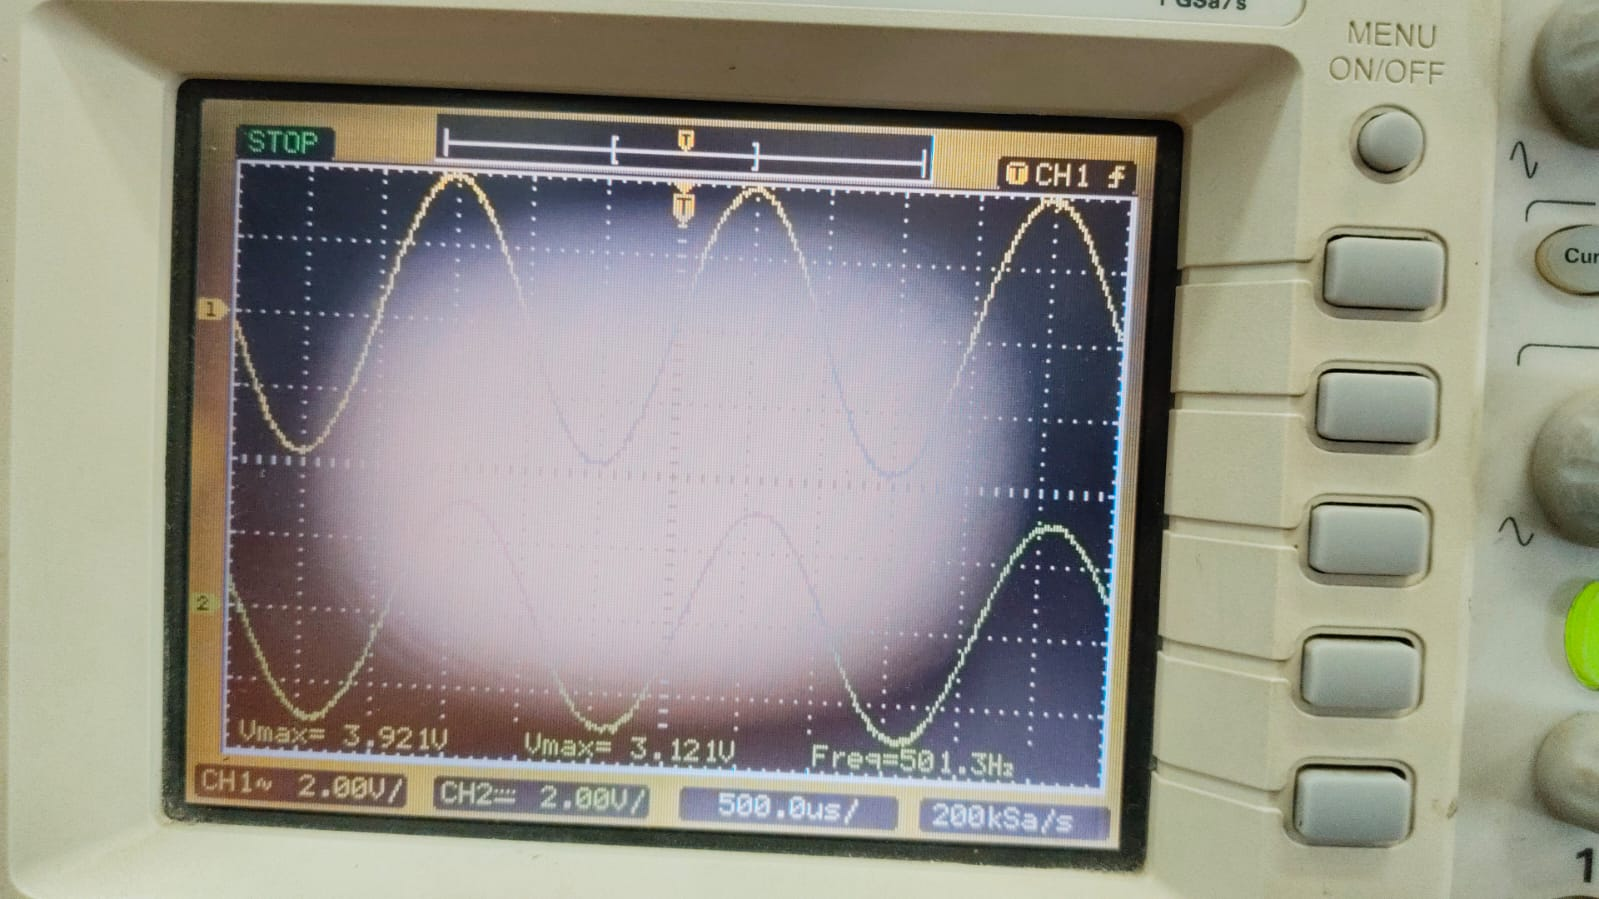
\includegraphics[width=0.45\textwidth]{figs/bpf_between_1.jpeg}
    }
    \hfill
    \subfigure[]{
        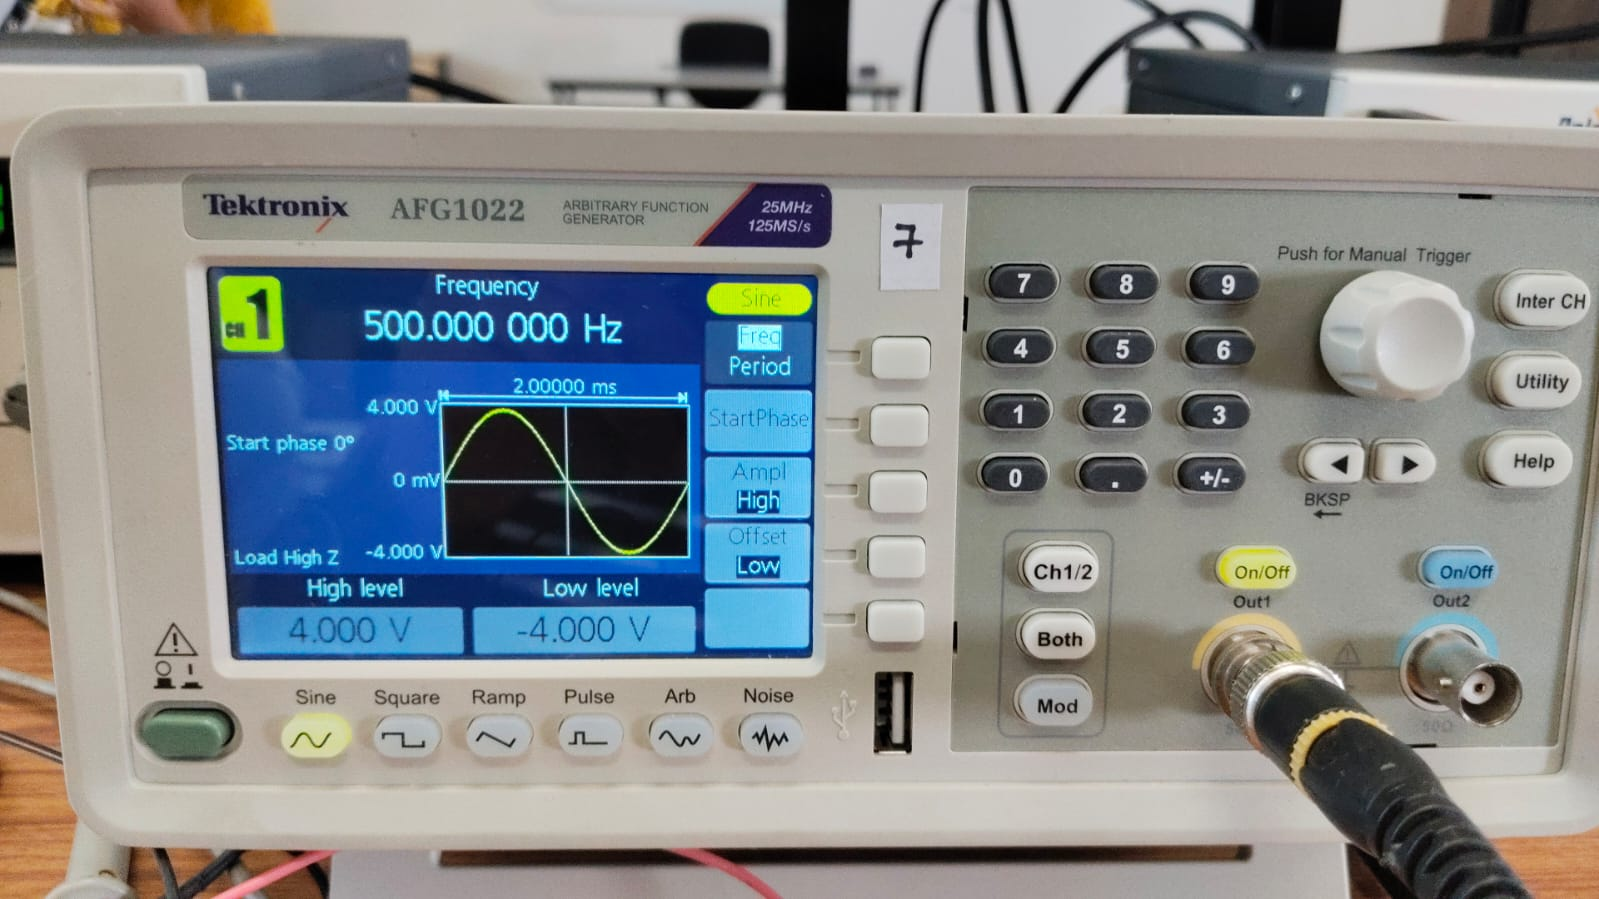
\includegraphics[width=0.45\textwidth]{figs/bpf_input_between_1.jpeg}
    }
\end{figure}
\begin{figure}[H]
    \centering
    \subfigure[]{
        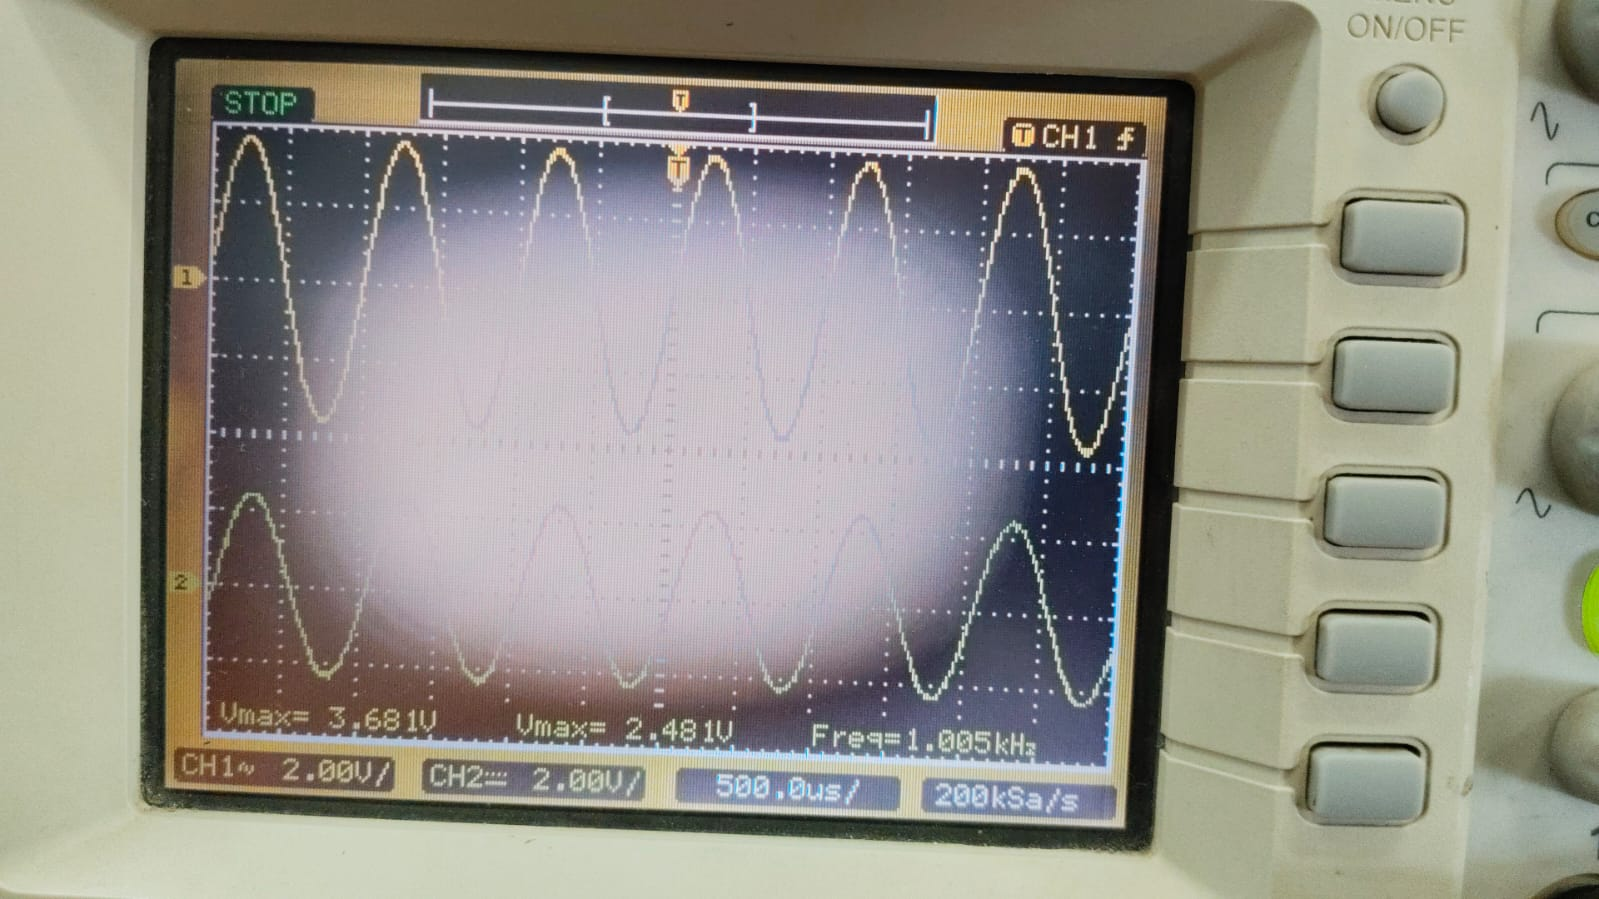
\includegraphics[width=0.45\textwidth]{figs/bpf_between_6.jpeg}
    }
    \hfill
    \subfigure[]{
        \includegraphics[width=0.45\textwidth]{figs/bpf_input_between_6.jpeg}
    }
\end{figure}
\begin{figure}[H]
    \centering
    \subfigure[]{
        \includegraphics[width=0.45\textwidth]{figs/bpf_hpf_cutoff.jpeg}
    }
    \hfill
    \subfigure[]{
        \includegraphics[width=0.45\textwidth]{figs/bpf_input_hpf_cutoff.jpeg}
    }
\end{figure}
\begin{figure}[H]
    \centering
    \subfigure[]{
        \includegraphics[width=0.45\textwidth]{figs/bpf_more_2.jpeg}
    }
    \hfill
    \subfigure[]{
        \includegraphics[width=0.45\textwidth]{figs/bpf_input_more_2.jpeg}
    }
\end{figure}
\begin{figure}[H]
    \centering
    \subfigure[]{
        \includegraphics[width=0.45\textwidth]{figs/bpf_more_1.jpeg}
    }
    \hfill
    \subfigure[]{
        \includegraphics[width=0.45\textwidth]{figs/bpf_input_more_1.jpeg}
    }
\end{figure}
\begin{figure}[H]
    \centering
    \includegraphics[width=\textwidth]{figs/band.png}
    \caption{Bode plot for BPF}
\end{figure}
\section{Observations and Results}
\begin{itemize}
    \item Plot the frequency response of HPF, LPF, and BPF.
    \item Compare the experimental and theoretical cutoff frequencies.
    \item Verify if the BPF passes the expected frequency range.
\end{itemize}

\section{Conclusion}
\begin{itemize}
    \item The experiment verifies the cascading method to form a bandpass filter.
    \item The experimental results should match the theoretical calculations.
    \item Sallen-Key topology provides good stability and response.
\end{itemize}

\end{document}

